\newpage
\section{Attività}
\subsection{Introduzione}
Questa sezione descriverà le operazioni che l'utente può svolgere all'interno di \progetto.
\\Per ogni operazione viene fornita:
\begin{itemize}
	\item una descrizione;
	\item un diagramma di attività;
	\item uno o più eventuali mockup.
\end{itemize}
I mockup hanno lo scopo di chiarificare la struttura della single-page \progetto. Il \glo{Gruppo}{gruppo} si riserva di poter modificare alcuni elementi grafici quando il prodotto sarà progettato nel dettaglio.
\\Le operazioni più complesse nei diagrammi di attività presentano uno sfondo di colore azzurro e sono ulteriormente descritte da sotto-diagrammi. \\ \\
%
Di seguito vengono mostrati due mockup che evidenziano come verrà organizzata l'interfaccia grafica nel progetto \progetto.
\begin{figure}[H]
	\centering
	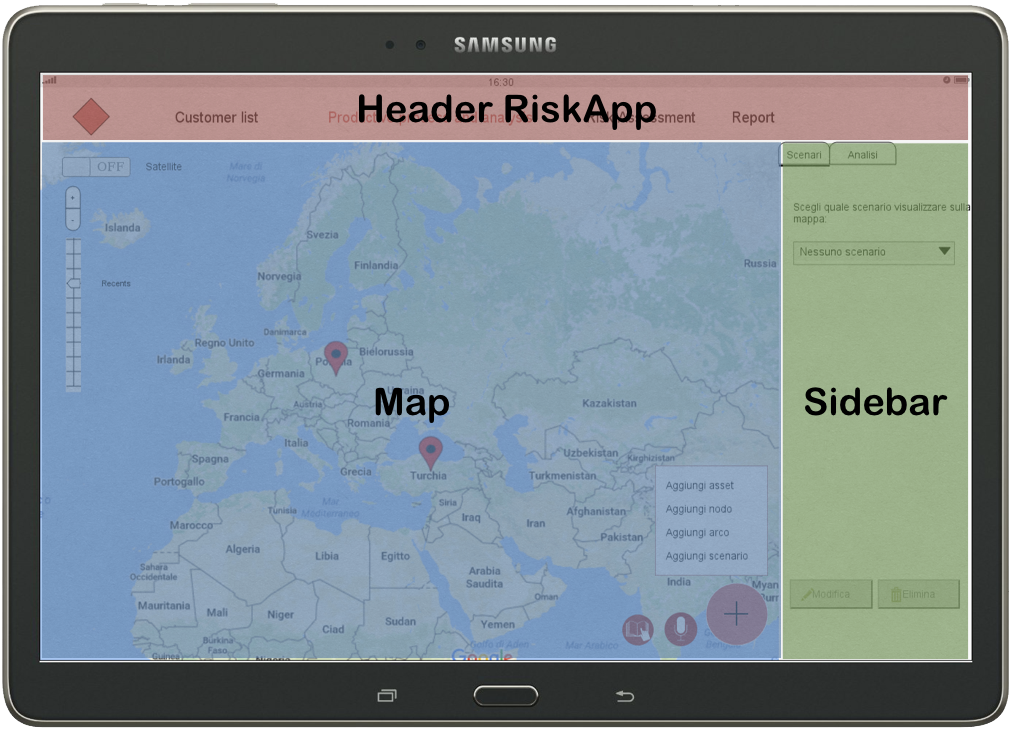
\includegraphics[scale=0.4]{img/MockUp/MockupConLayerHi}
	\caption{Mockup interfaccia grafica ad alto livello}
\end{figure}

\begin{figure}[H]
	\centering
	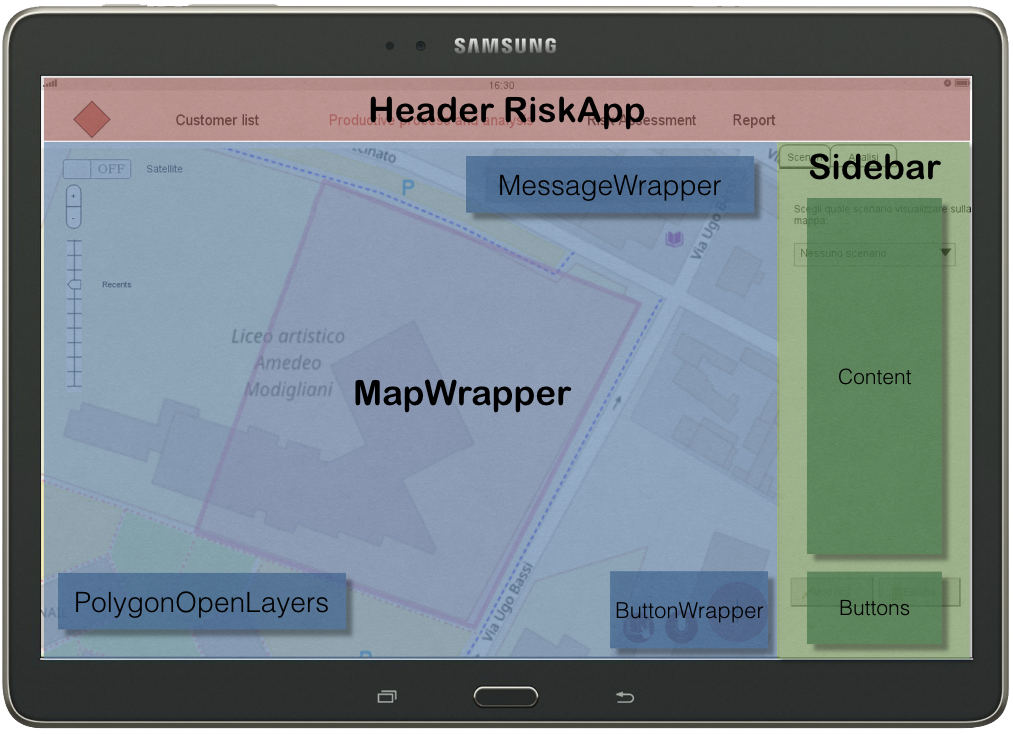
\includegraphics[scale=0.4]{img/MockUp/MockupConLayerLow}
	\caption{Mockup interfaccia grafica basso livello}
\end{figure}

\subsection{Visualizzazione di default}
\progetto{} sarà sviluppato come una single-page e tutte le operazioni che l'utente può svolgere sono attuabili a partire dalla visualizzazione di default (si veda il relativo mockup).
L'utente, dopo aver acceduto a \progetto, potrà:
\begin{itemize}
	\item interagire ripetutamente con la mappa:
		\begin{itemize}
			\item aumentando/diminuendo il livello di zoom;
			\item spostandosi sulla mappa;
			\item attivando/disattivando la vista satellitare.
		\end{itemize}
	\item svolgere ripetutamente una o più tra le seguenti operazioni:
	\begin{itemize}
		\item selezionare un \glo{Asset}{asset}, \glo{Nodo}{nodo}, \glo{Arco}{arco}, scenario;
		\item aggiungere asset, nodi, archi, scenari;
		\item gestire le analisi;
		\item avviare il tutorial o l'assistente vocale.
	\end{itemize}
\end{itemize} 



\begin{figure}[H]
	\centering
	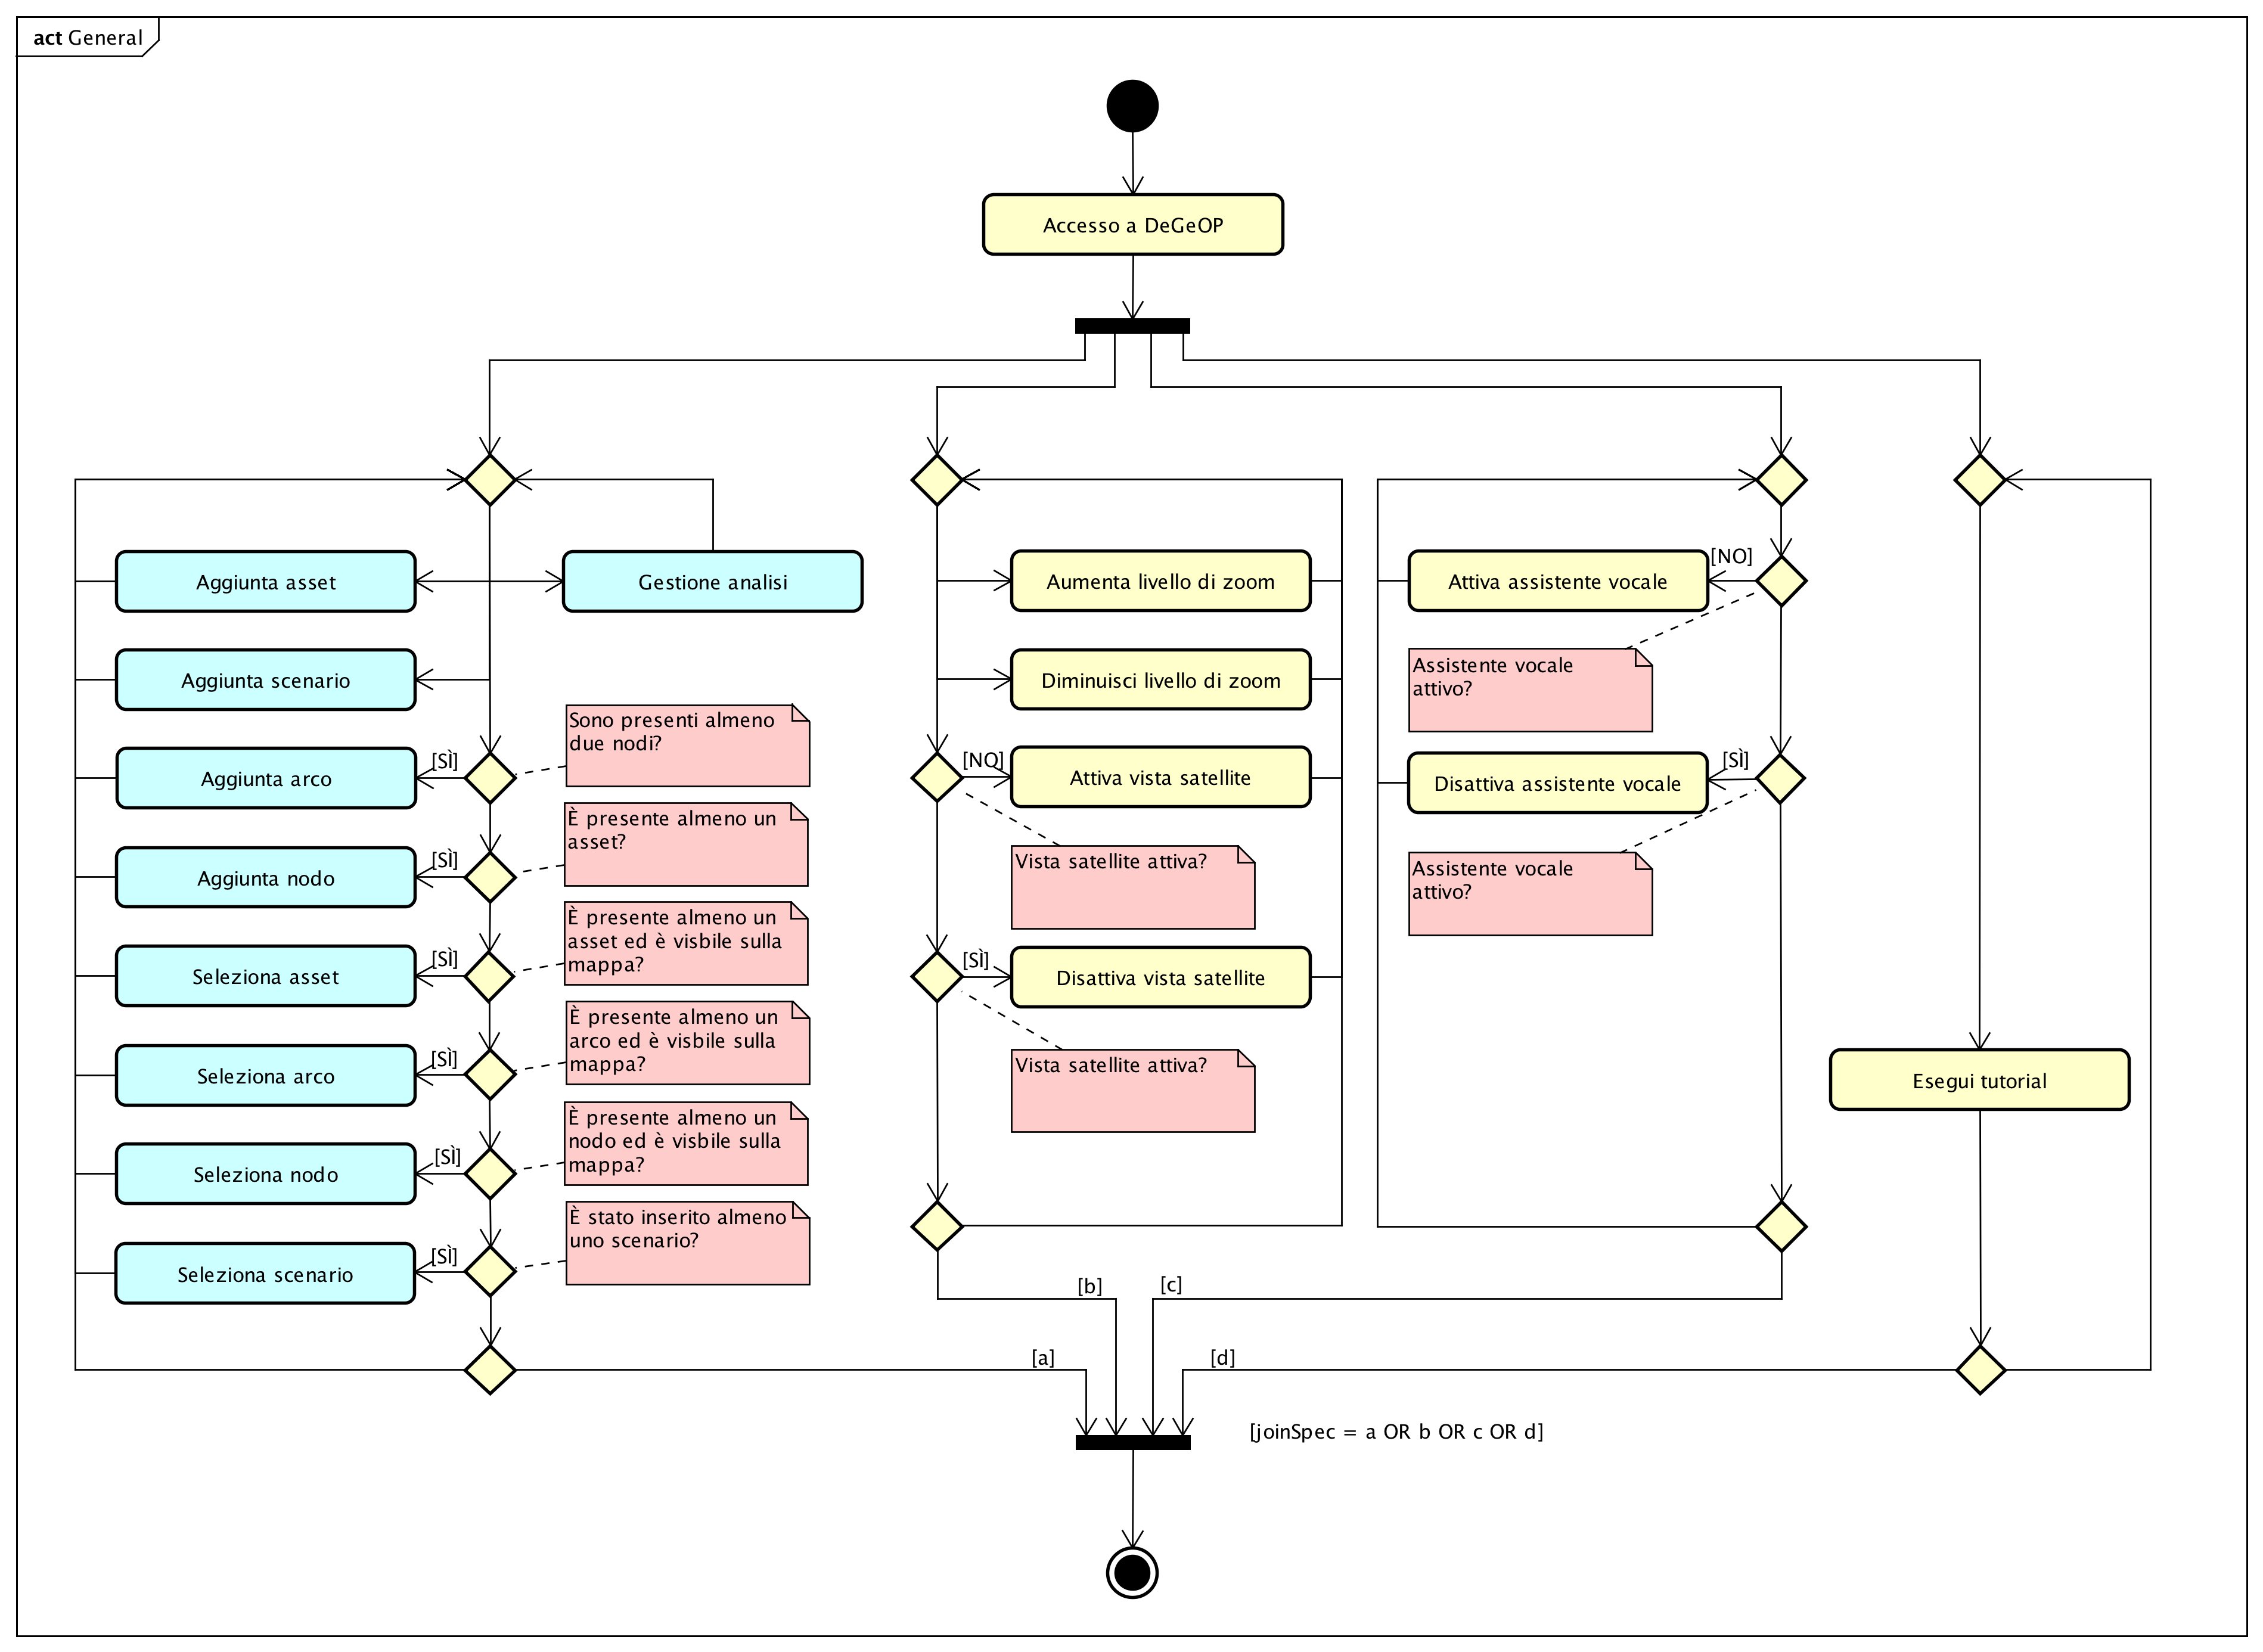
\includegraphics[width=\textwidth]{img/DiagrammiDiAttivita/GeneralActivities.png}
	\caption{Diagramma delle attività generale}
\end{figure}

\begin{figure}[H]
	\centering
	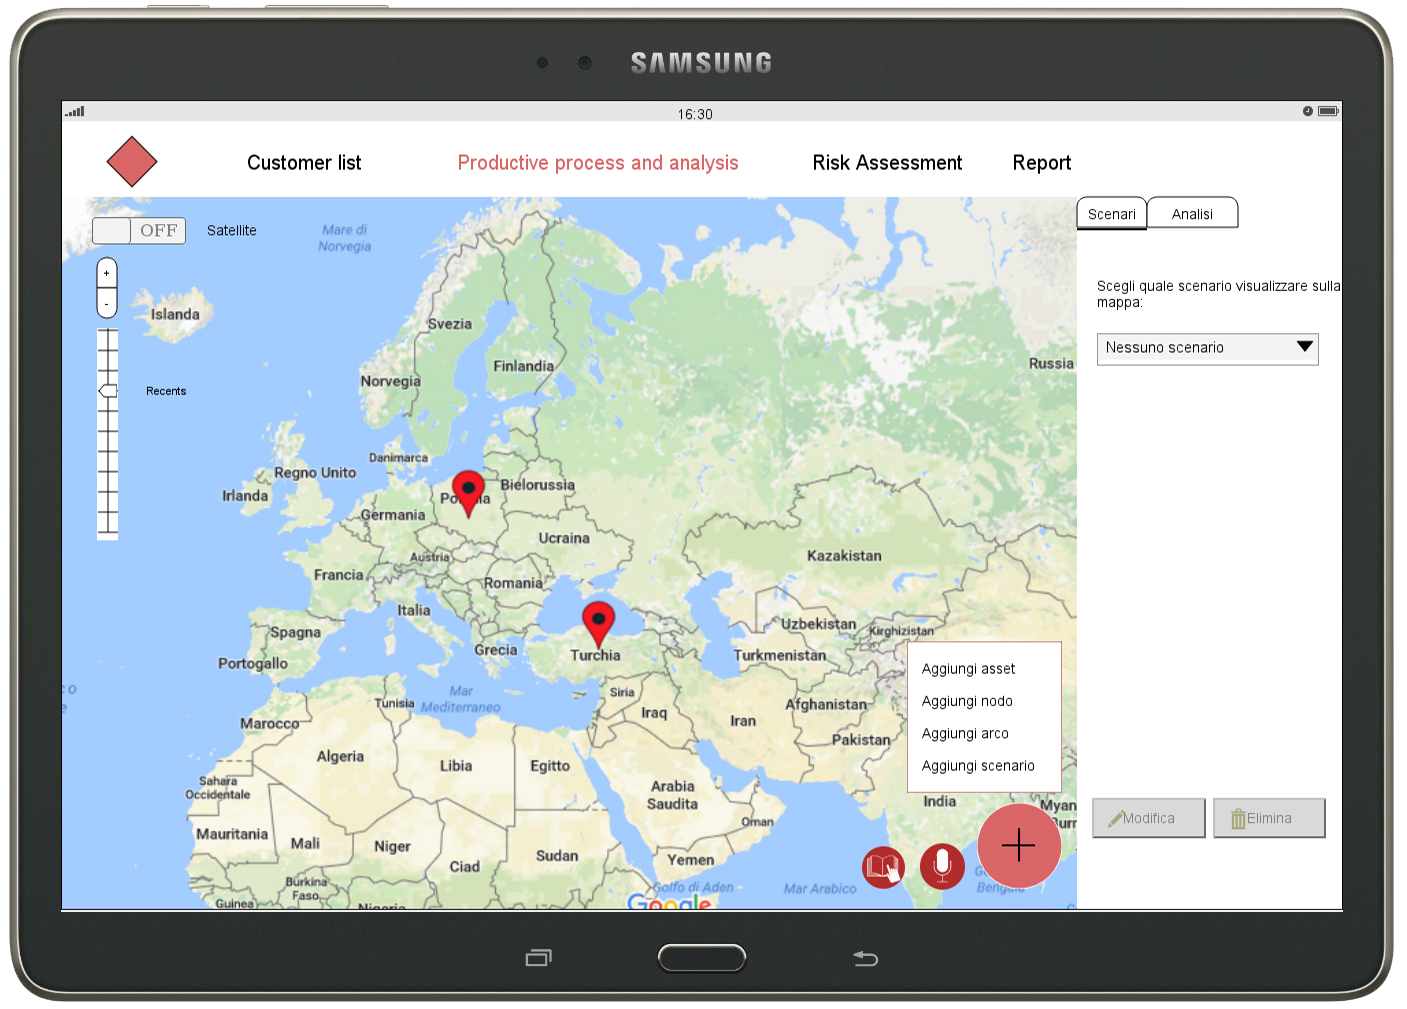
\includegraphics[width=\textwidth]{img/MockUp/m0.jpg}
	\caption{Mockup per la visualizzazione di default}
\end{figure}

\newpage
\subsection{Aggiunta asset}
Per aggiungere un asset l'utente dovrà disegnare il perimetro dell'asset sulla mappa, compilarne i dati e confermare l'inserimento. In caso di dati non corretti, l'inserimento potrebbe non andare a buon fine: verrà visualizzato un messaggio di errore e l'utente sarà tenuto a correggere eventuali errori o incompletezze.
In ogni momento l'utente può annullare l'inserimento. Il sistema richiede una conferma per portare a termine tale operazione. 
\begin{figure}[H]
	\centering
	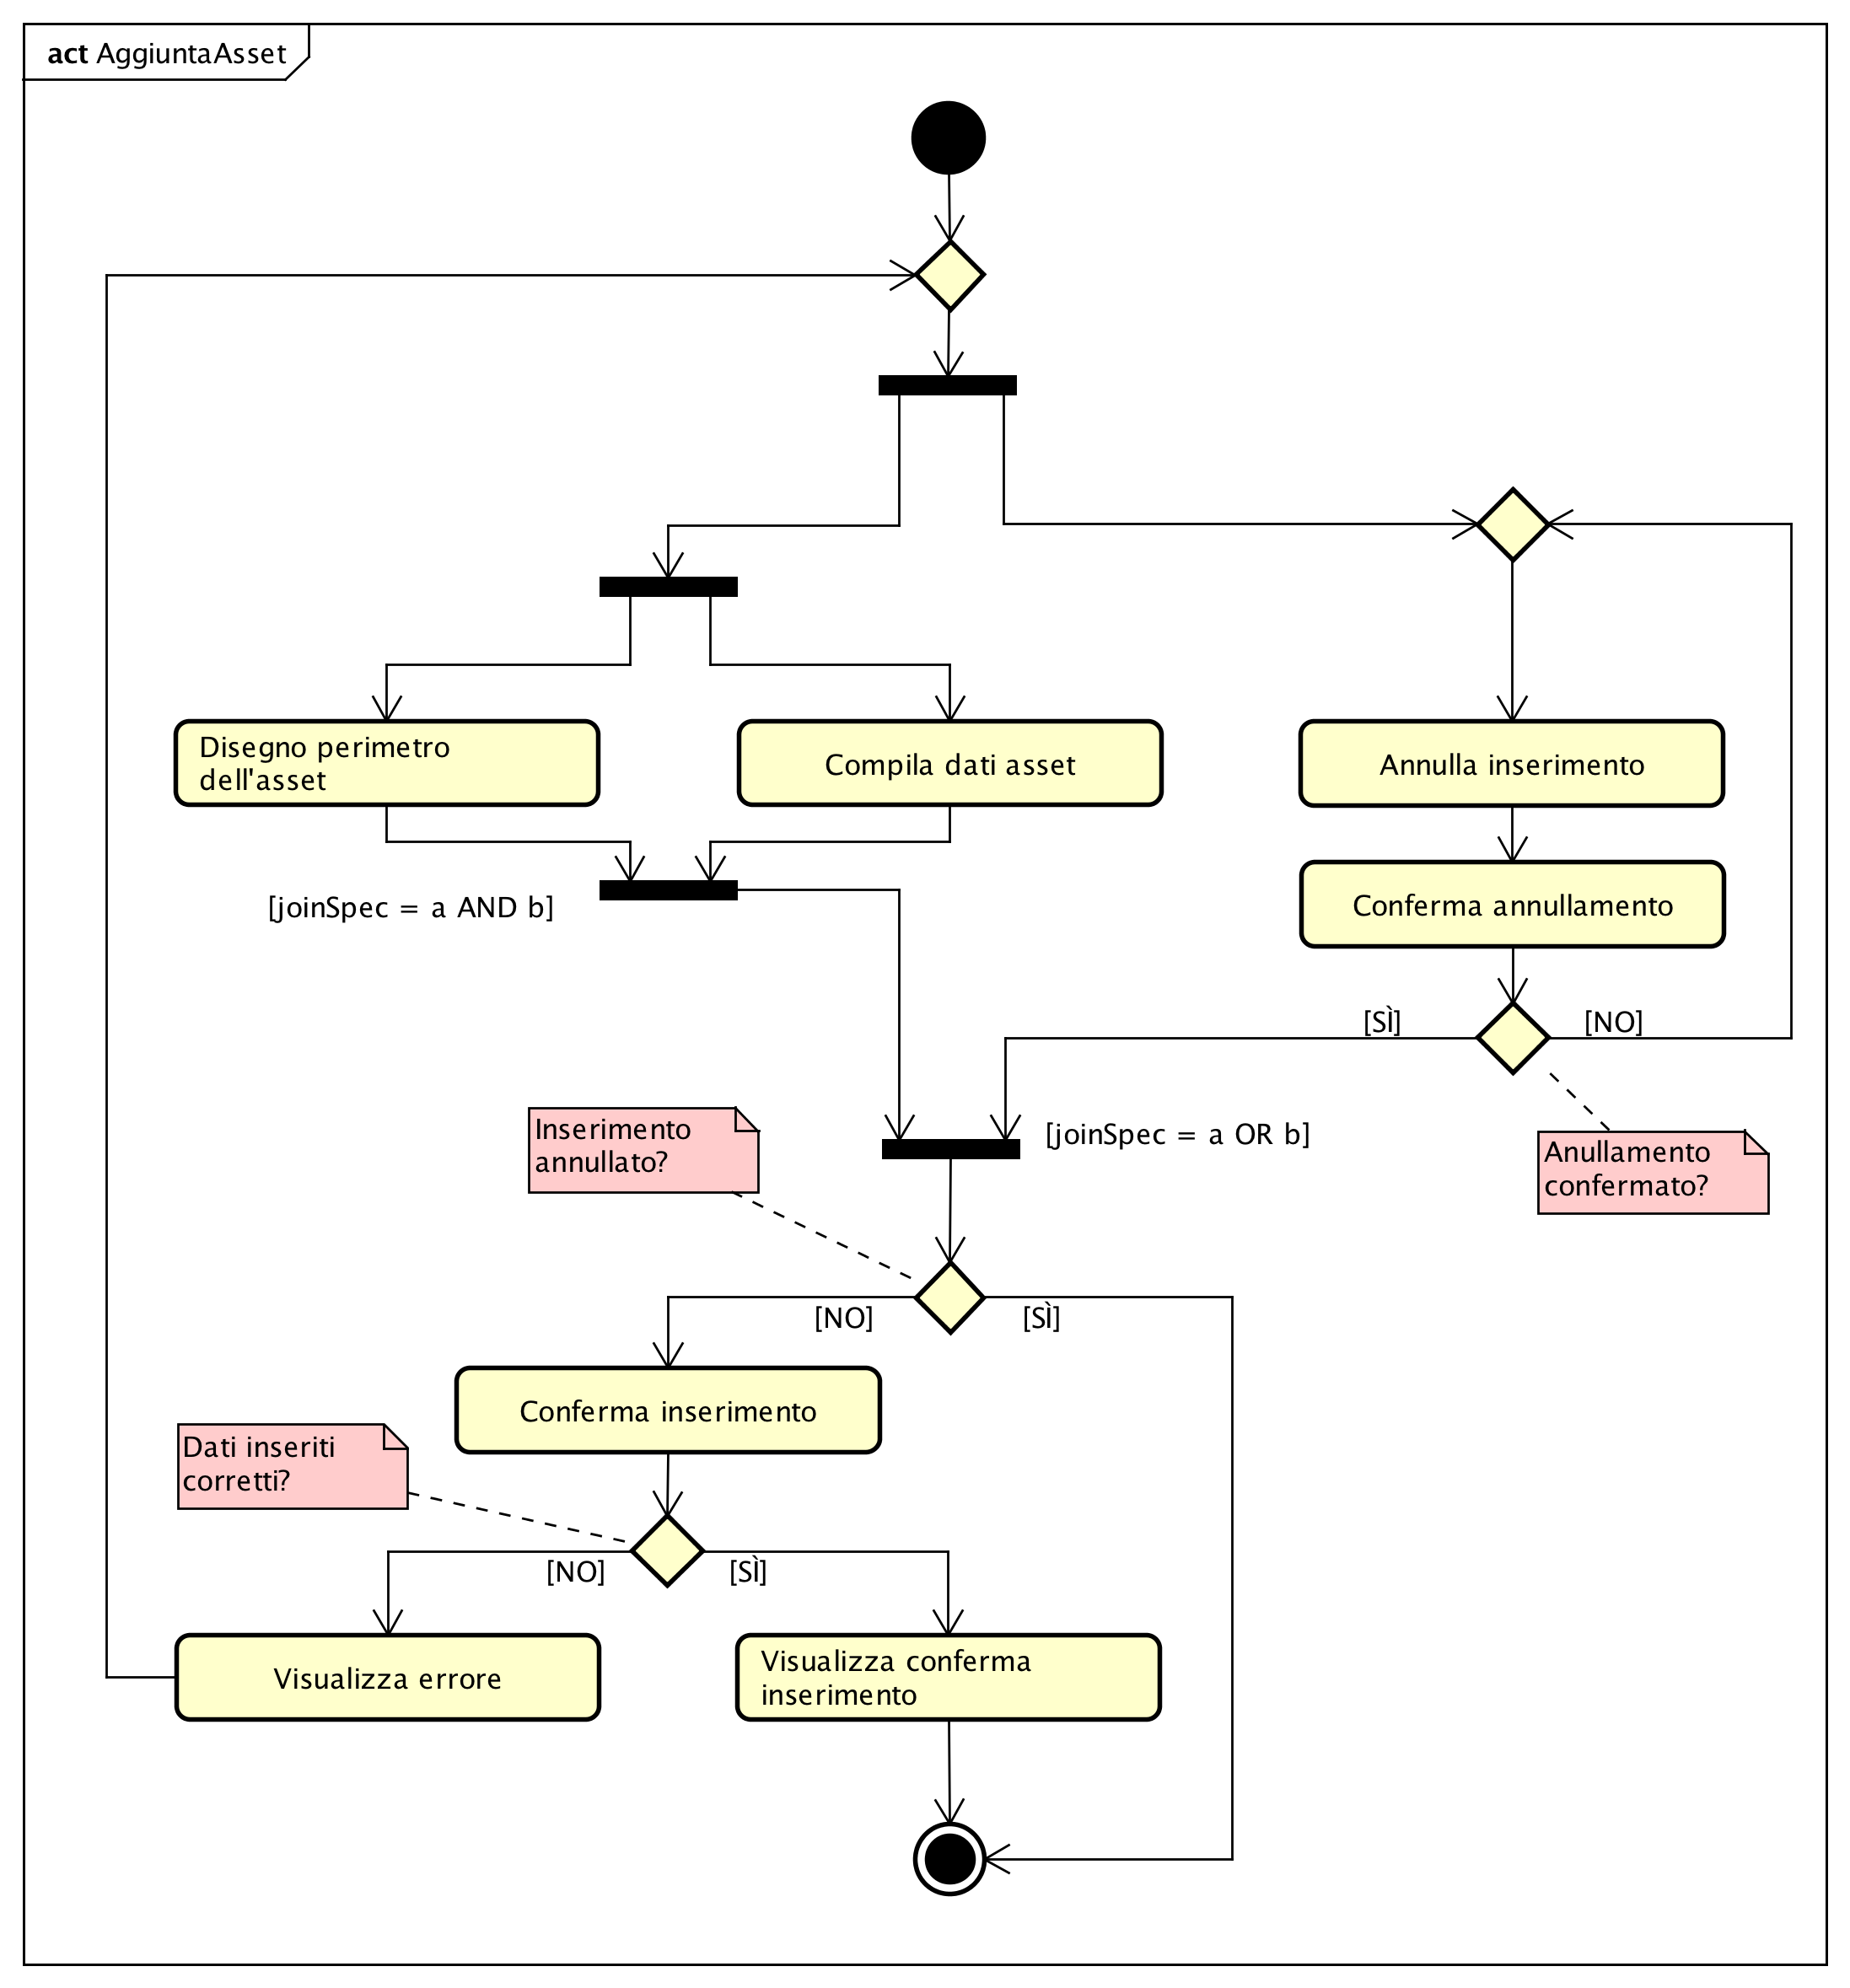
\includegraphics[width=\textwidth]{img/DiagrammiDiAttivita/AggiuntaAsset.png}
	\caption{Diagramma di attività per l'aggiunta di un asset}
\end{figure}
\begin{figure}[H]
	\centering
	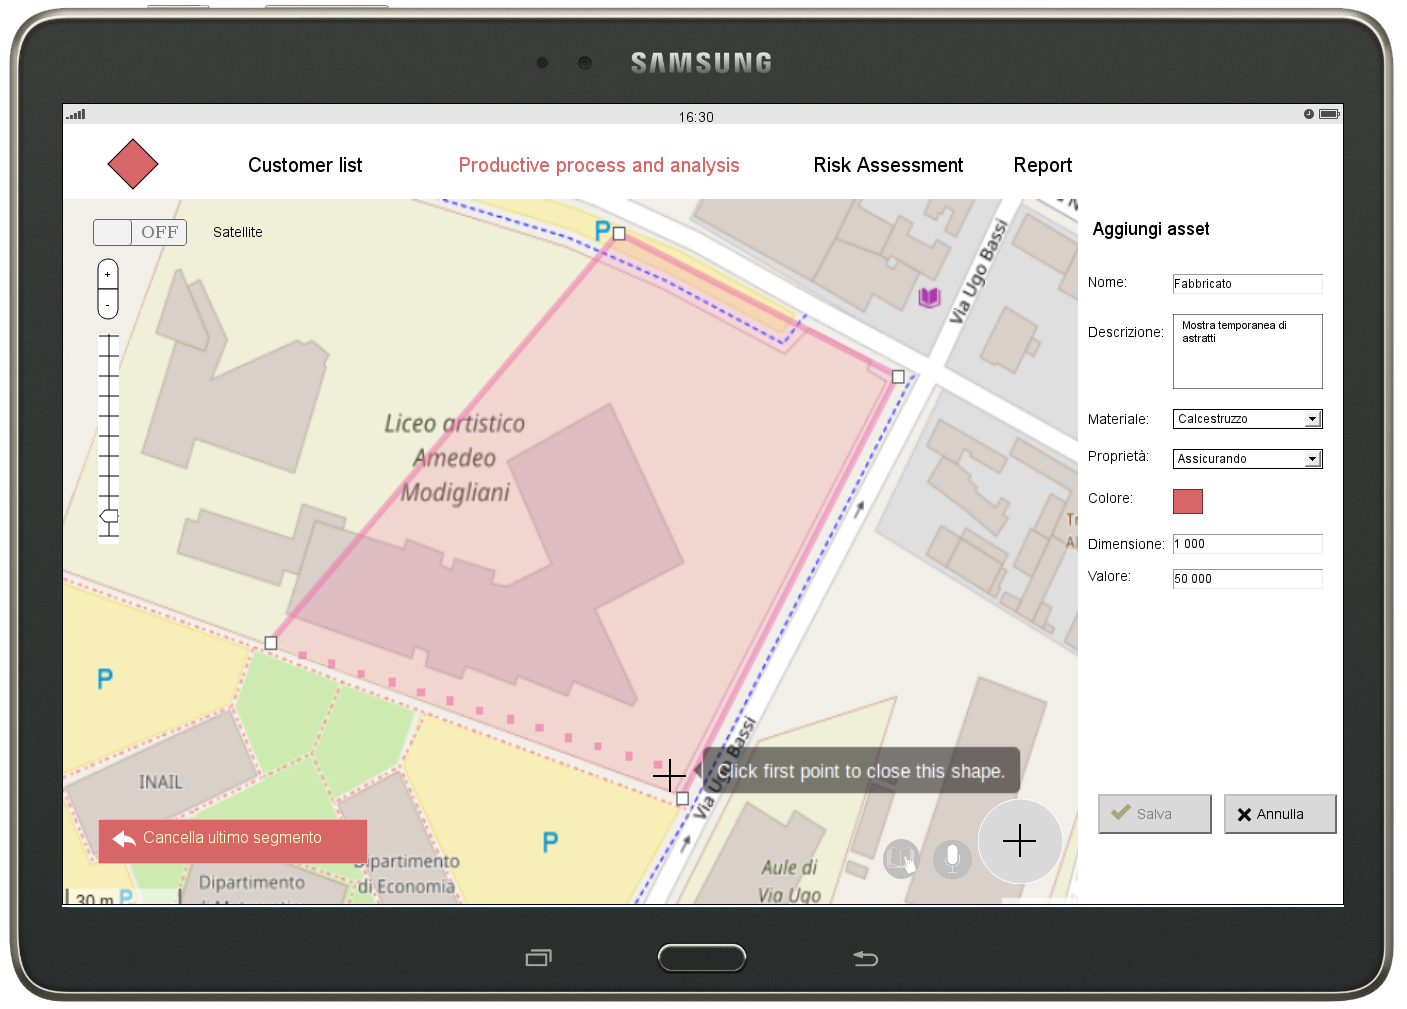
\includegraphics[scale=0.29]{img/MockUp/m4.png}
	\caption{Mockup per l'aggiunta dell'asset}
\end{figure}
\begin{figure}[H]
	\centering
	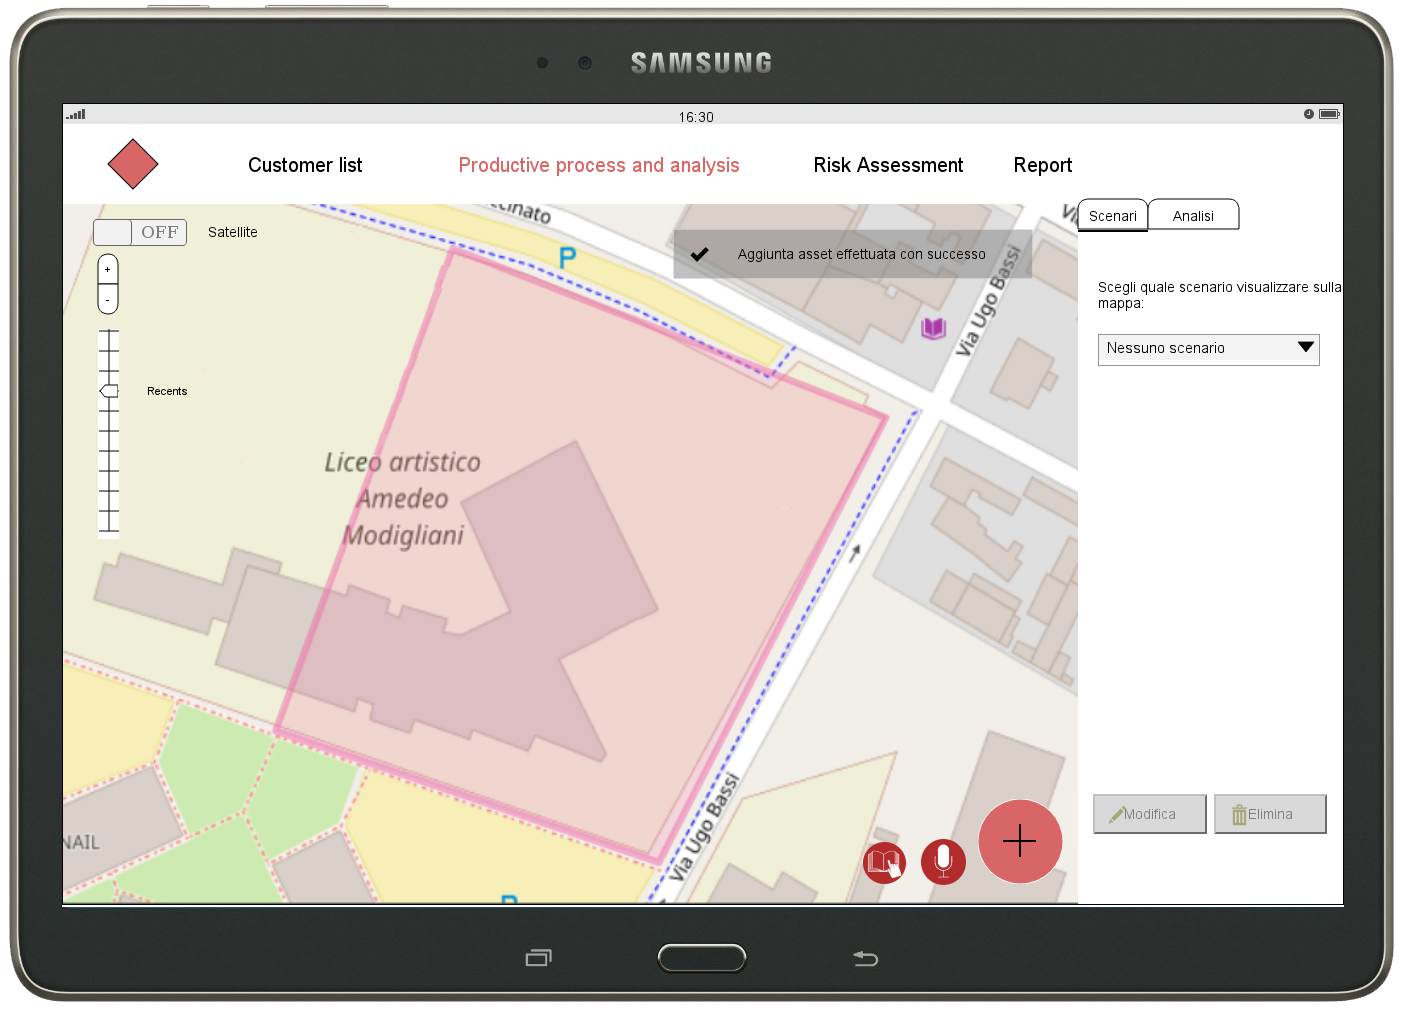
\includegraphics[scale=0.29]{img/MockUp/m5.png}
	\caption{Mockup per il successo dell'operazione di aggiunta asset}
\end{figure}
\begin{figure}[H]
	\centering
	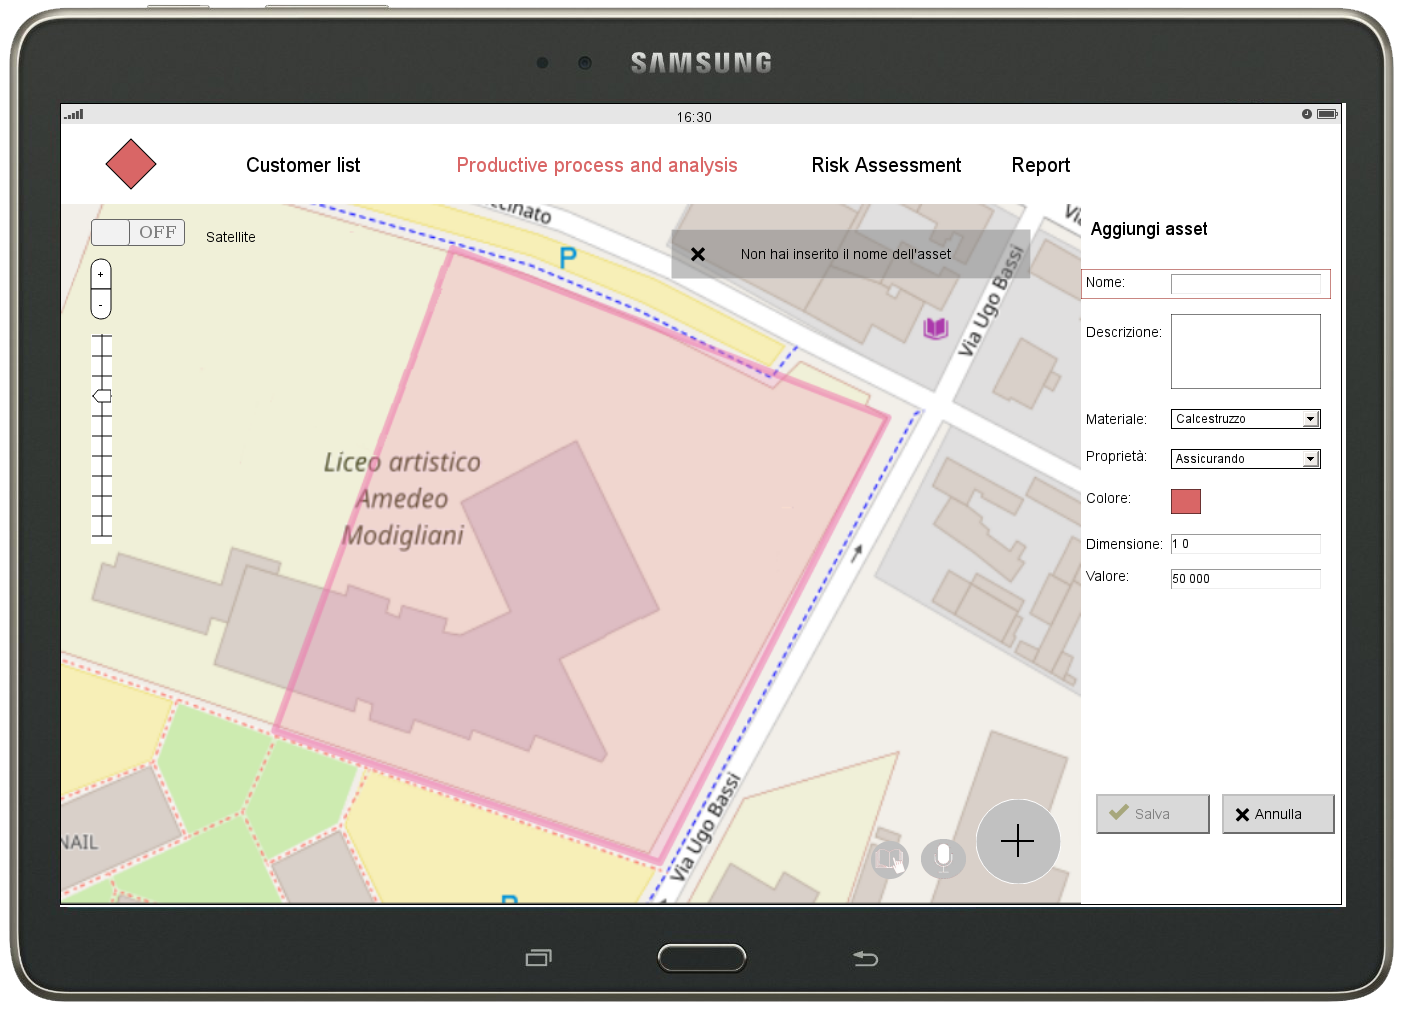
\includegraphics[scale=0.29]{img/MockUp/m6.png}
	\caption{Mockup per l'errore durante l'operazione di aggiunta asset}
\end{figure}

\newpage
\subsection{Aggiunta nodo}
Per aggiungere un nodo, l'utente dovrà posizionare il nodo all'interno dell'asset di appartenenza sulla mappa, compilarne i dati e confermare l'inserimento. In caso di dati non corretti, l'inserimento potrebbe non andare a buon fine: verrà visualizzato un messaggio di errore e l'utente sarà tenuto a correggere eventuali errori o incompletezze.
In ogni momento l'utente può annullare l'inserimento. Il sistema richiede una conferma per portare a termine tale operazione. 
\begin{figure}[H]
	\centering
	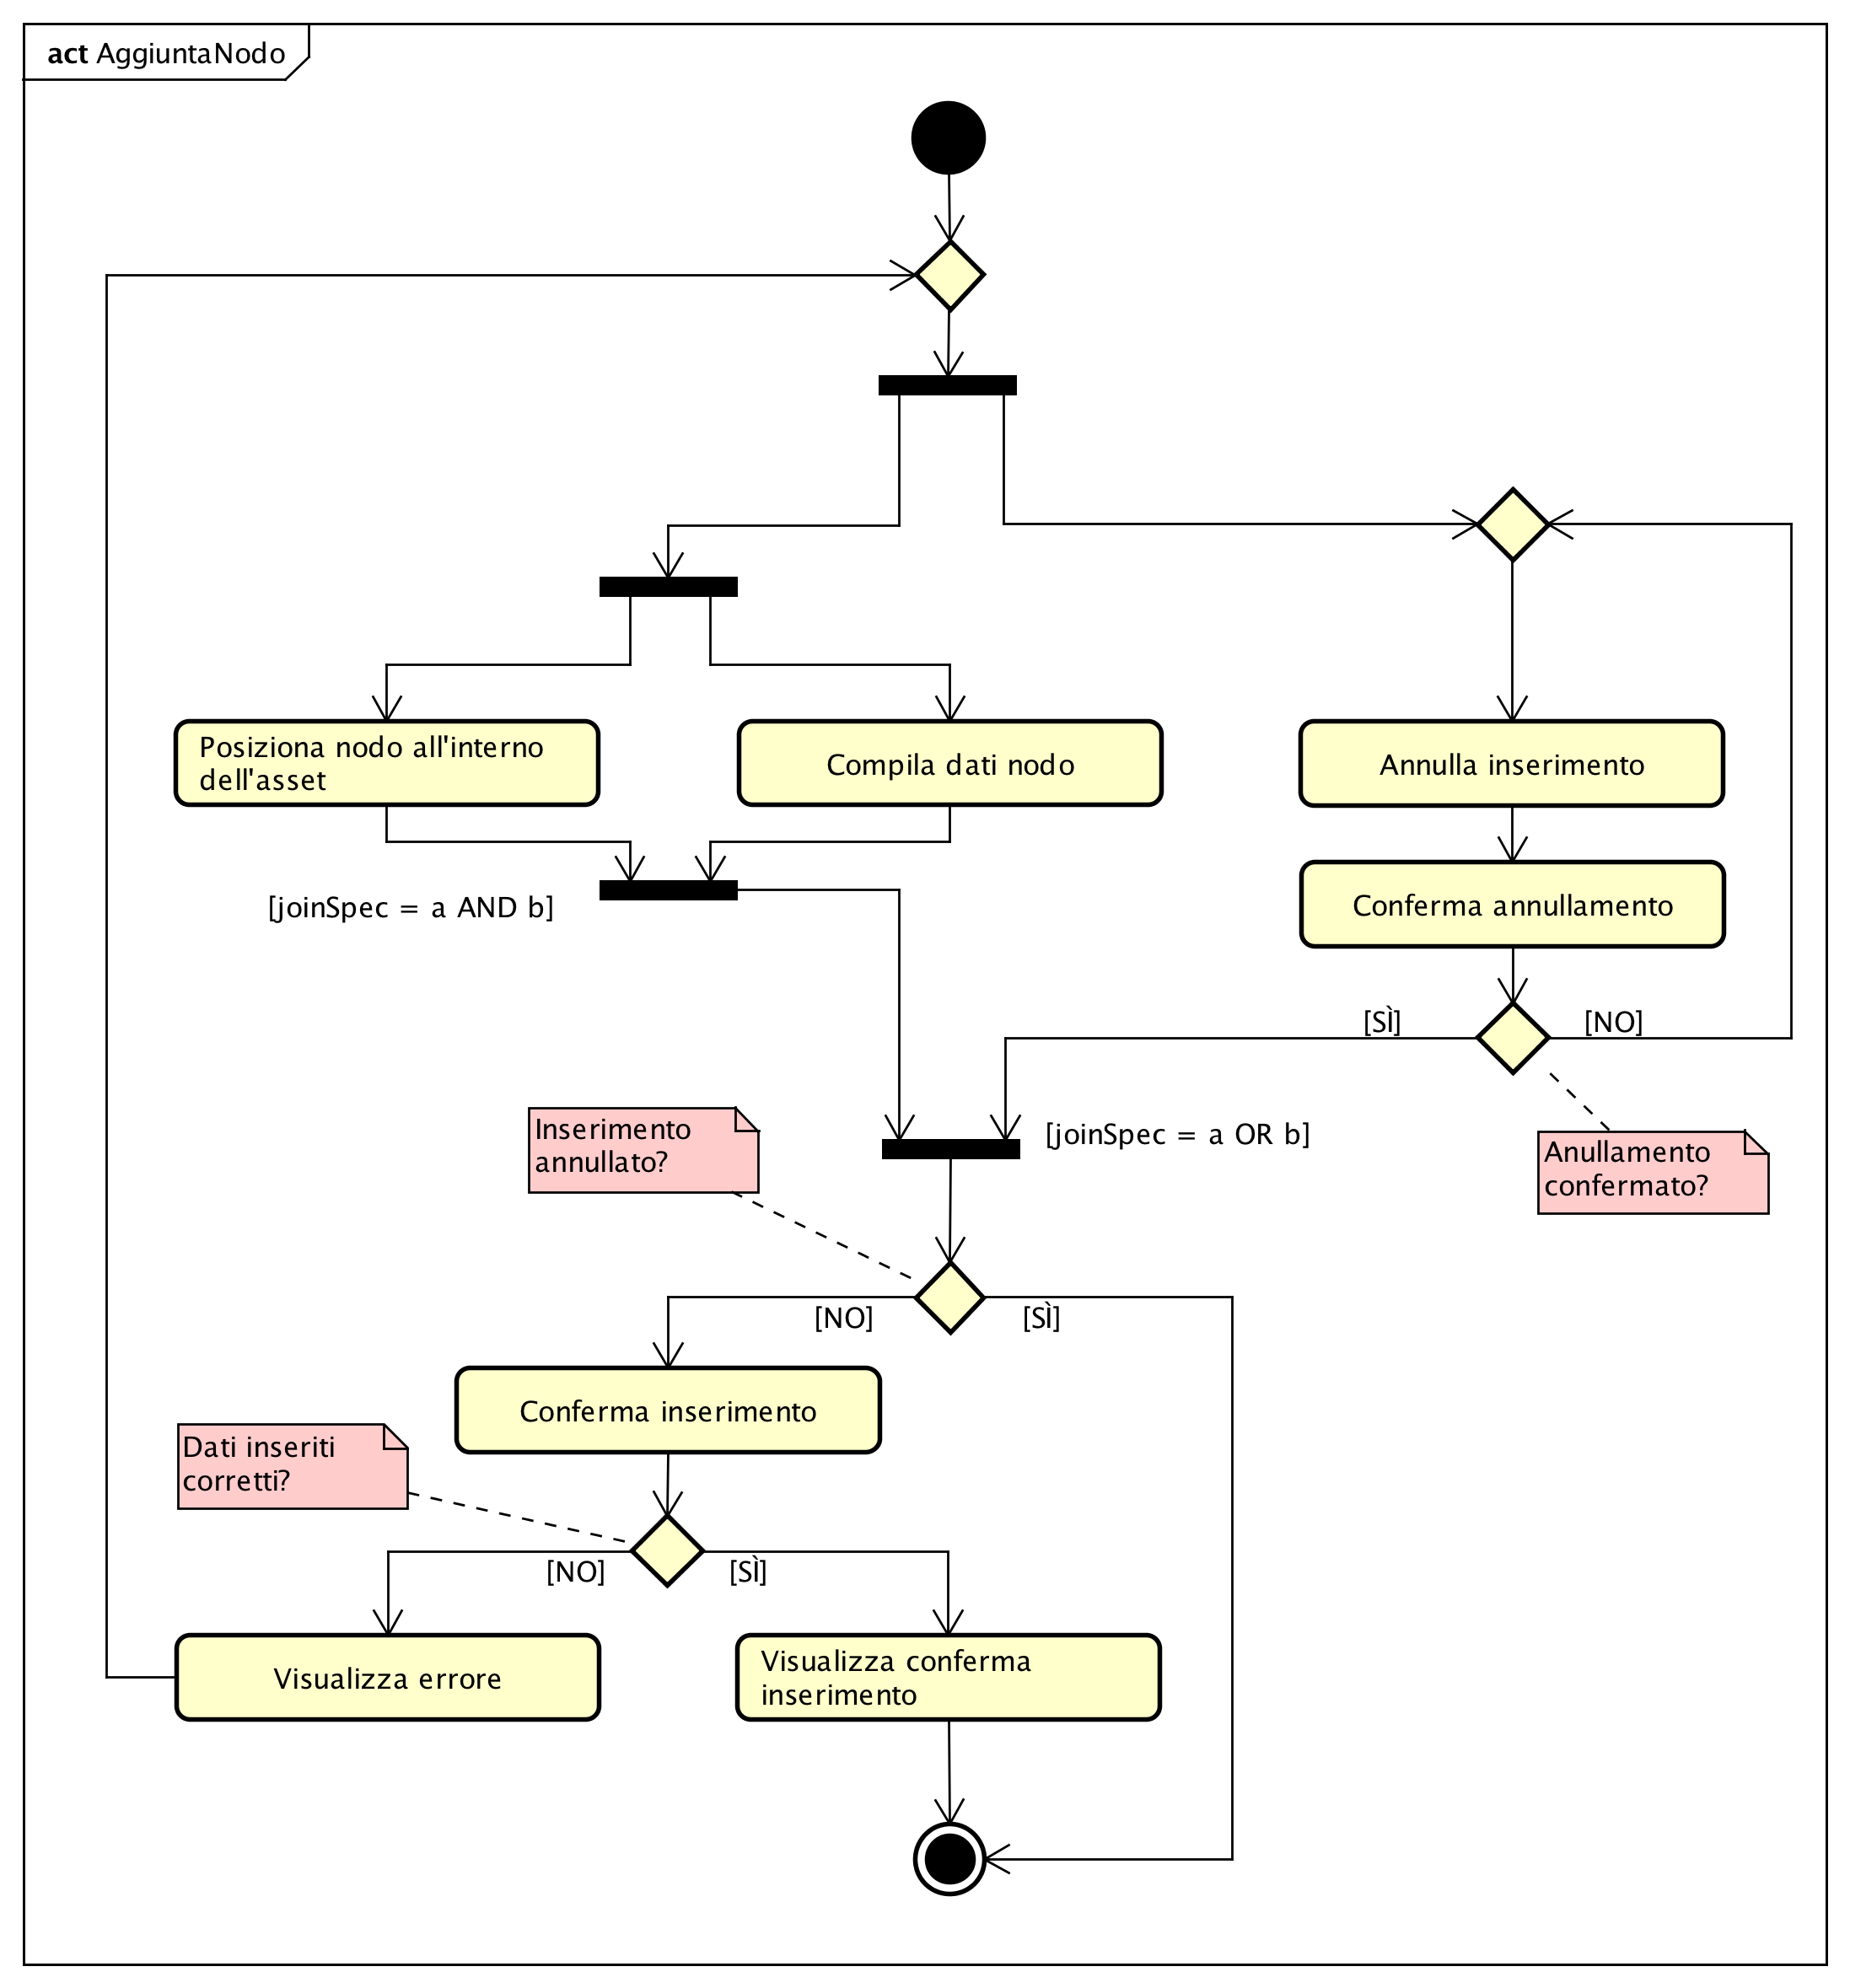
\includegraphics[width=\textwidth]{img/DiagrammiDiAttivita/AggiuntaNodo.png}
	\caption{Diagramma di attività per l'aggiunta di un nodo}
\end{figure}
\begin{figure}[H]
	\centering
	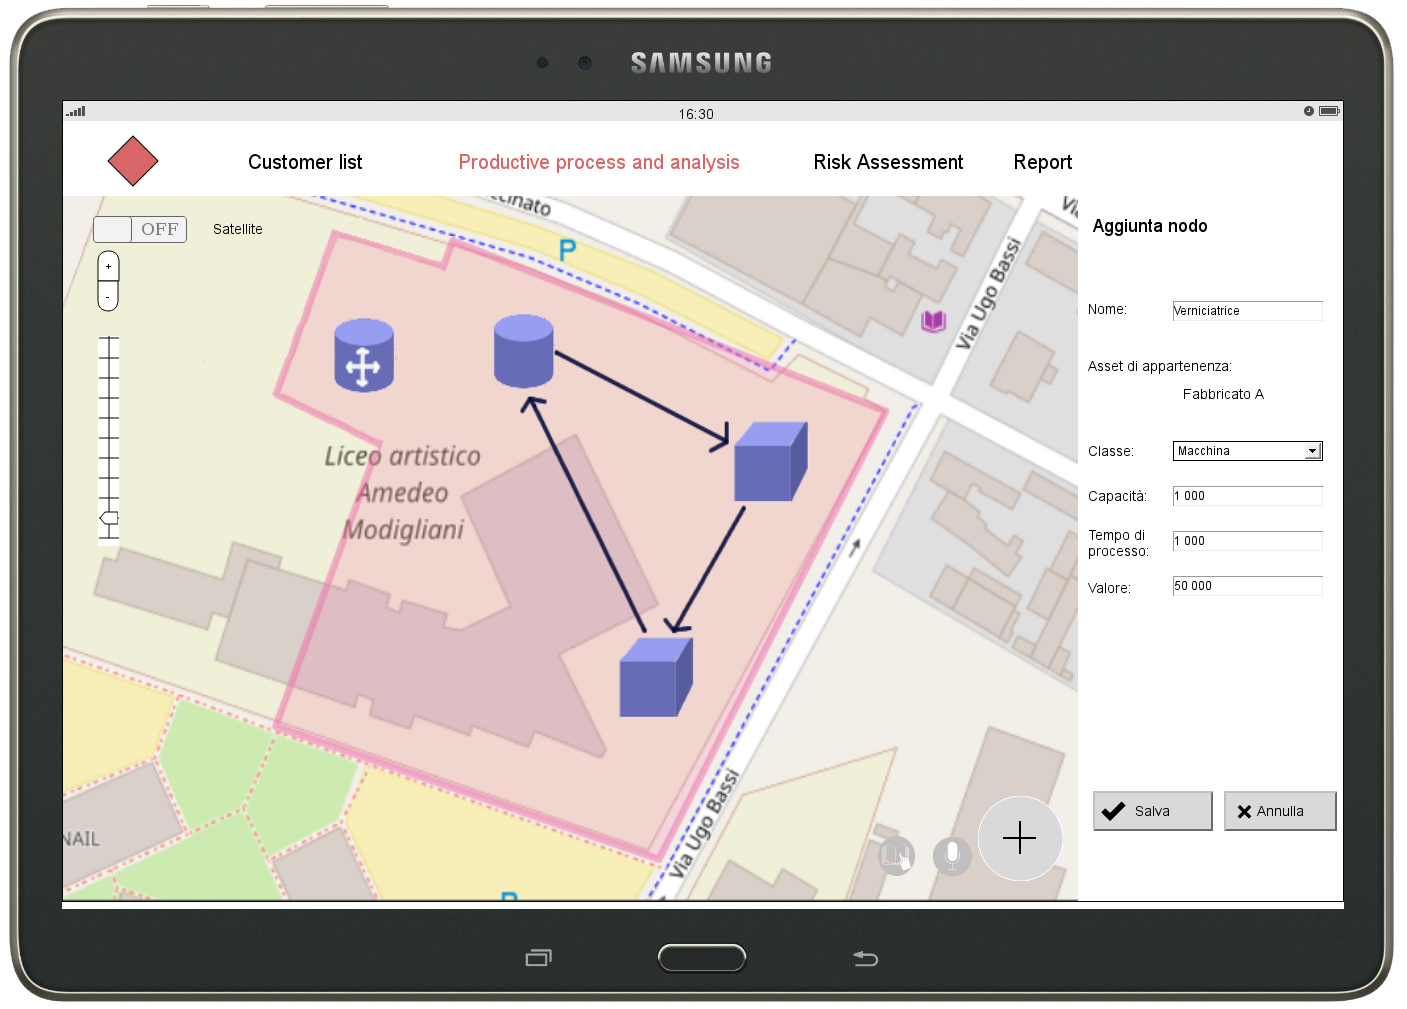
\includegraphics[width=\textwidth]{img/MockUp/m12.png}
	\caption{Mockup per l'aggiunta di un nodo}
\end{figure}

\newpage
\subsection{Aggiunta arco}
Per aggiungere un arco, l'utente dovrà disegnare l'arco sulla mappa, compilarne i dati e confermare l'inserimento. In caso di dati non corretti, l'inserimento potrebbe non andare a buon fine: verrà visualizzato un messaggio di errore e l'utente sarà tenuto a correggere eventuali errori o incompletezze.
In ogni momento l'utente può annullare l'inserimento. Il sistema richiede una conferma per portare a termine tale operazione.
\begin{figure}[H]
	\centering
	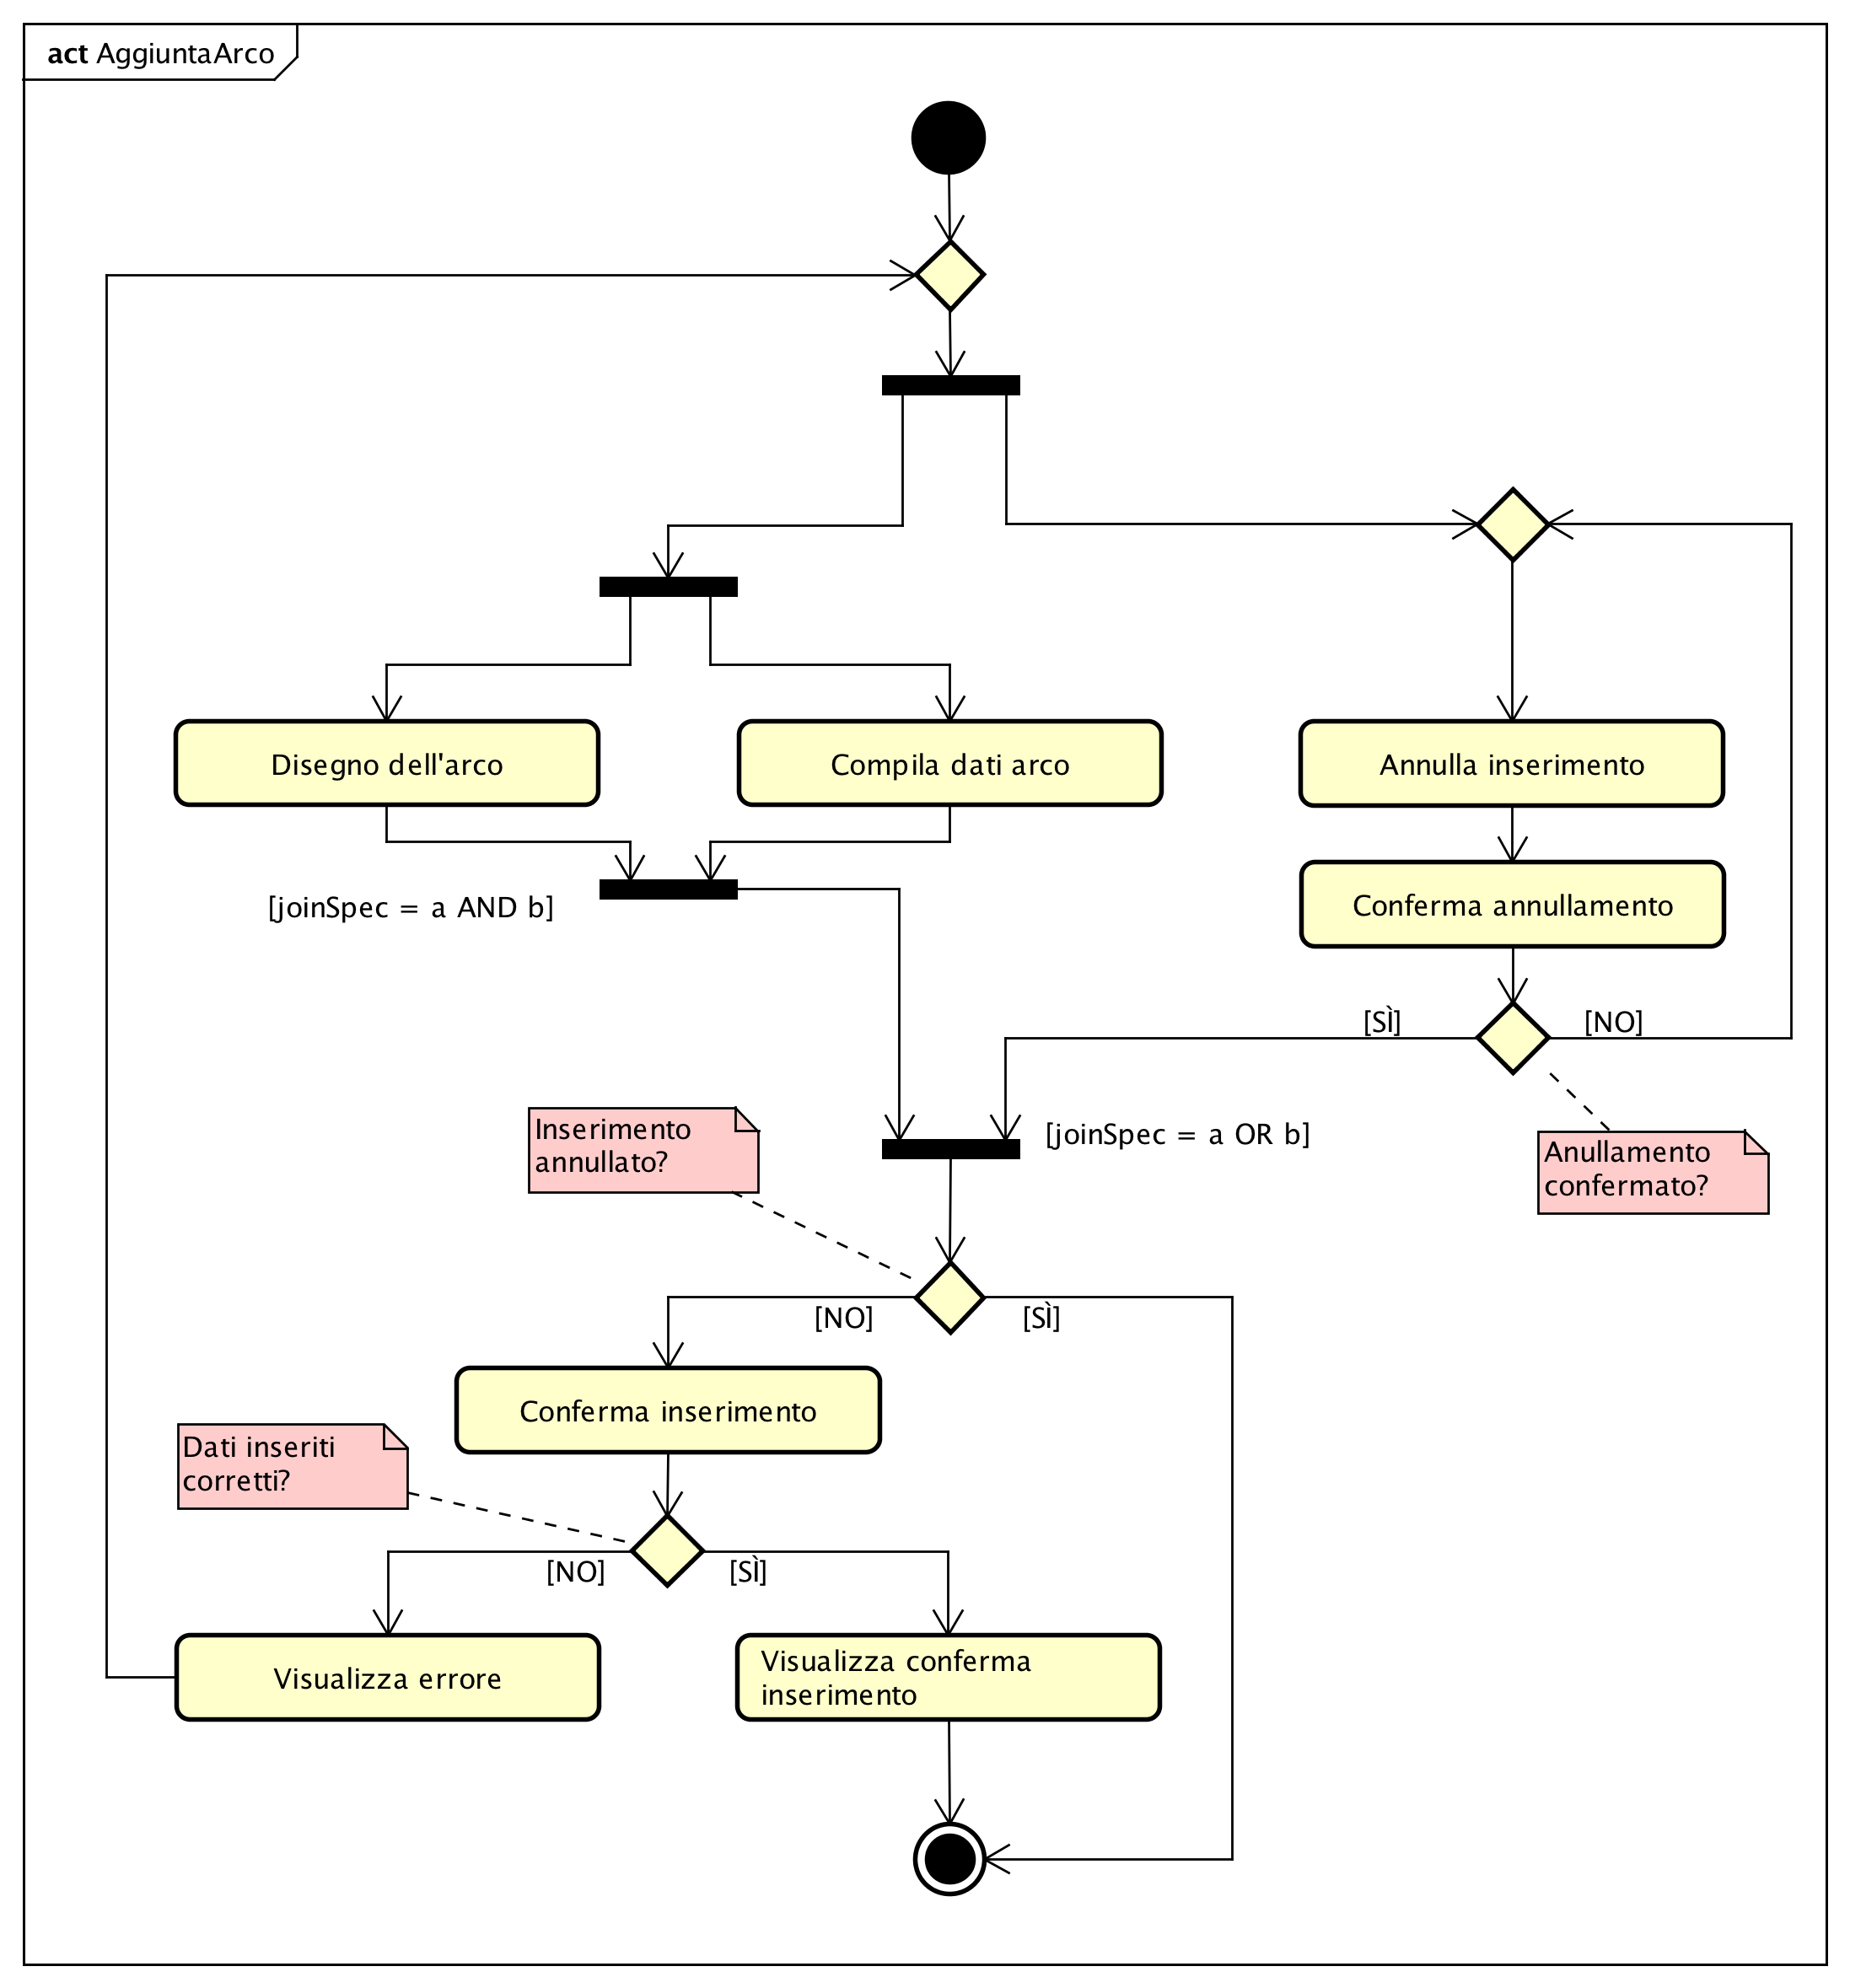
\includegraphics[width=\textwidth]{img/DiagrammiDiAttivita/AggiuntaArco.png}
	\caption{Diagramma di attività per l'aggiunta di un arco}
\end{figure}
\begin{figure}[H]
	\centering
	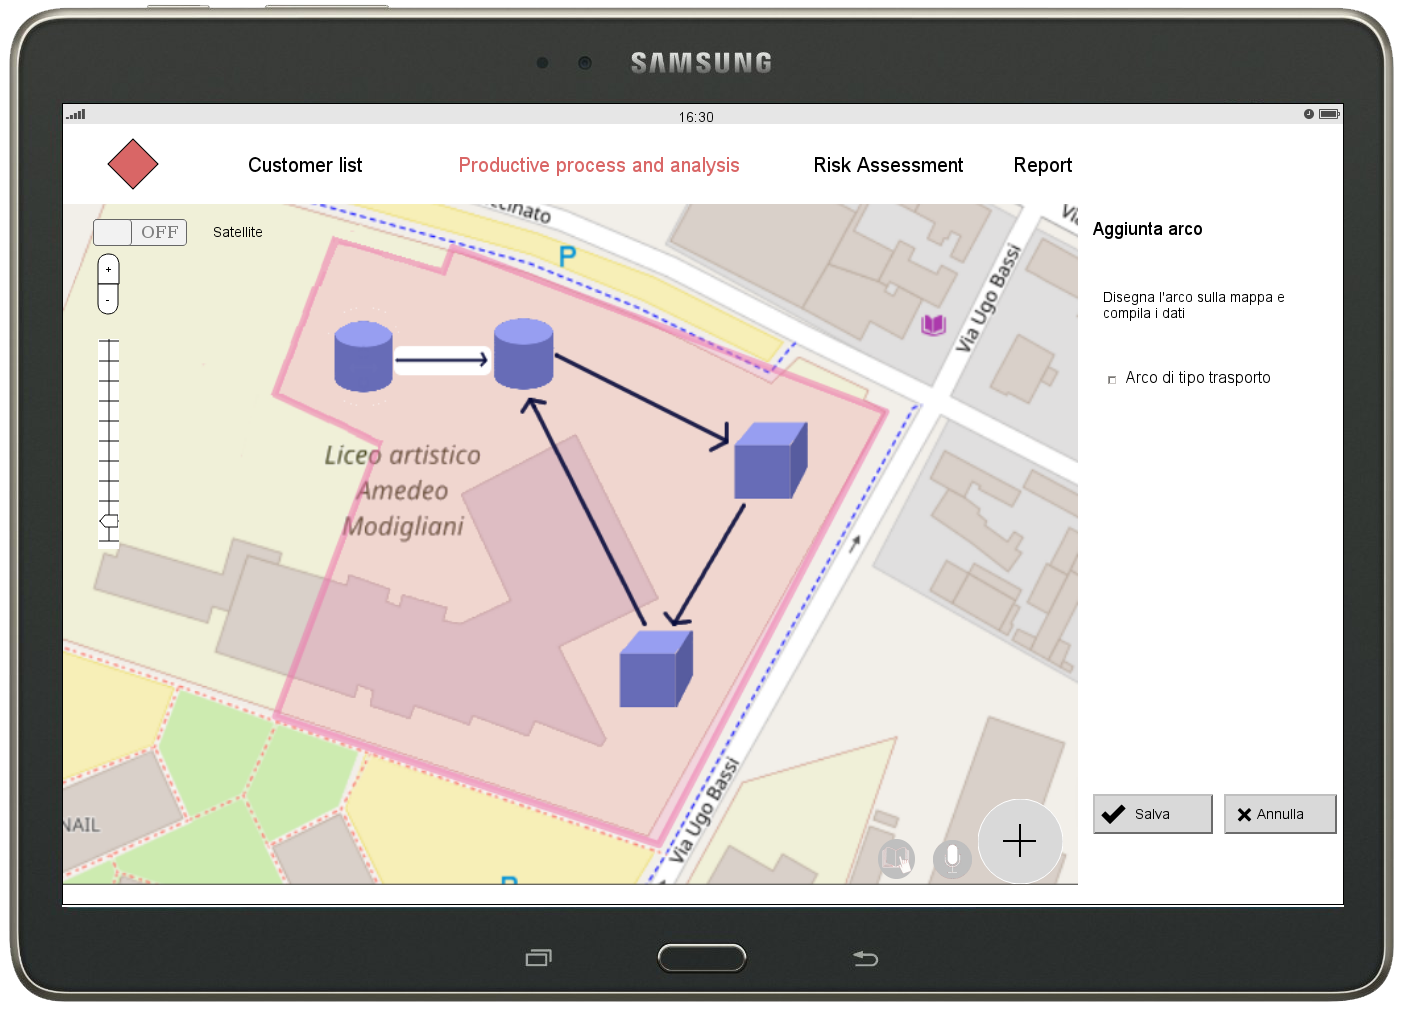
\includegraphics[width=\textwidth]{img/MockUp/m18.png}
	\caption{Mockup per l'aggiunta di un arco}
\end{figure}

\newpage
\subsection{Aggiunta scenario}
Per aggiungere uno scenario l'utente dovrà disegnare il perimetro dello scenario sulla mappa, compilarne i dati e confermare l'inserimento. In caso di dati non corretti, l'inserimento potrebbe non andare a buon fine: verrà visualizzato un messaggio di errore e l'utente sarà tenuto a correggere eventuali errori o incompletezze.
In ogni momento l'utente può annullare l'inserimento. Il sistema richiede una conferma per portare a termine tale operazione.
\begin{figure}[H]
	\centering
	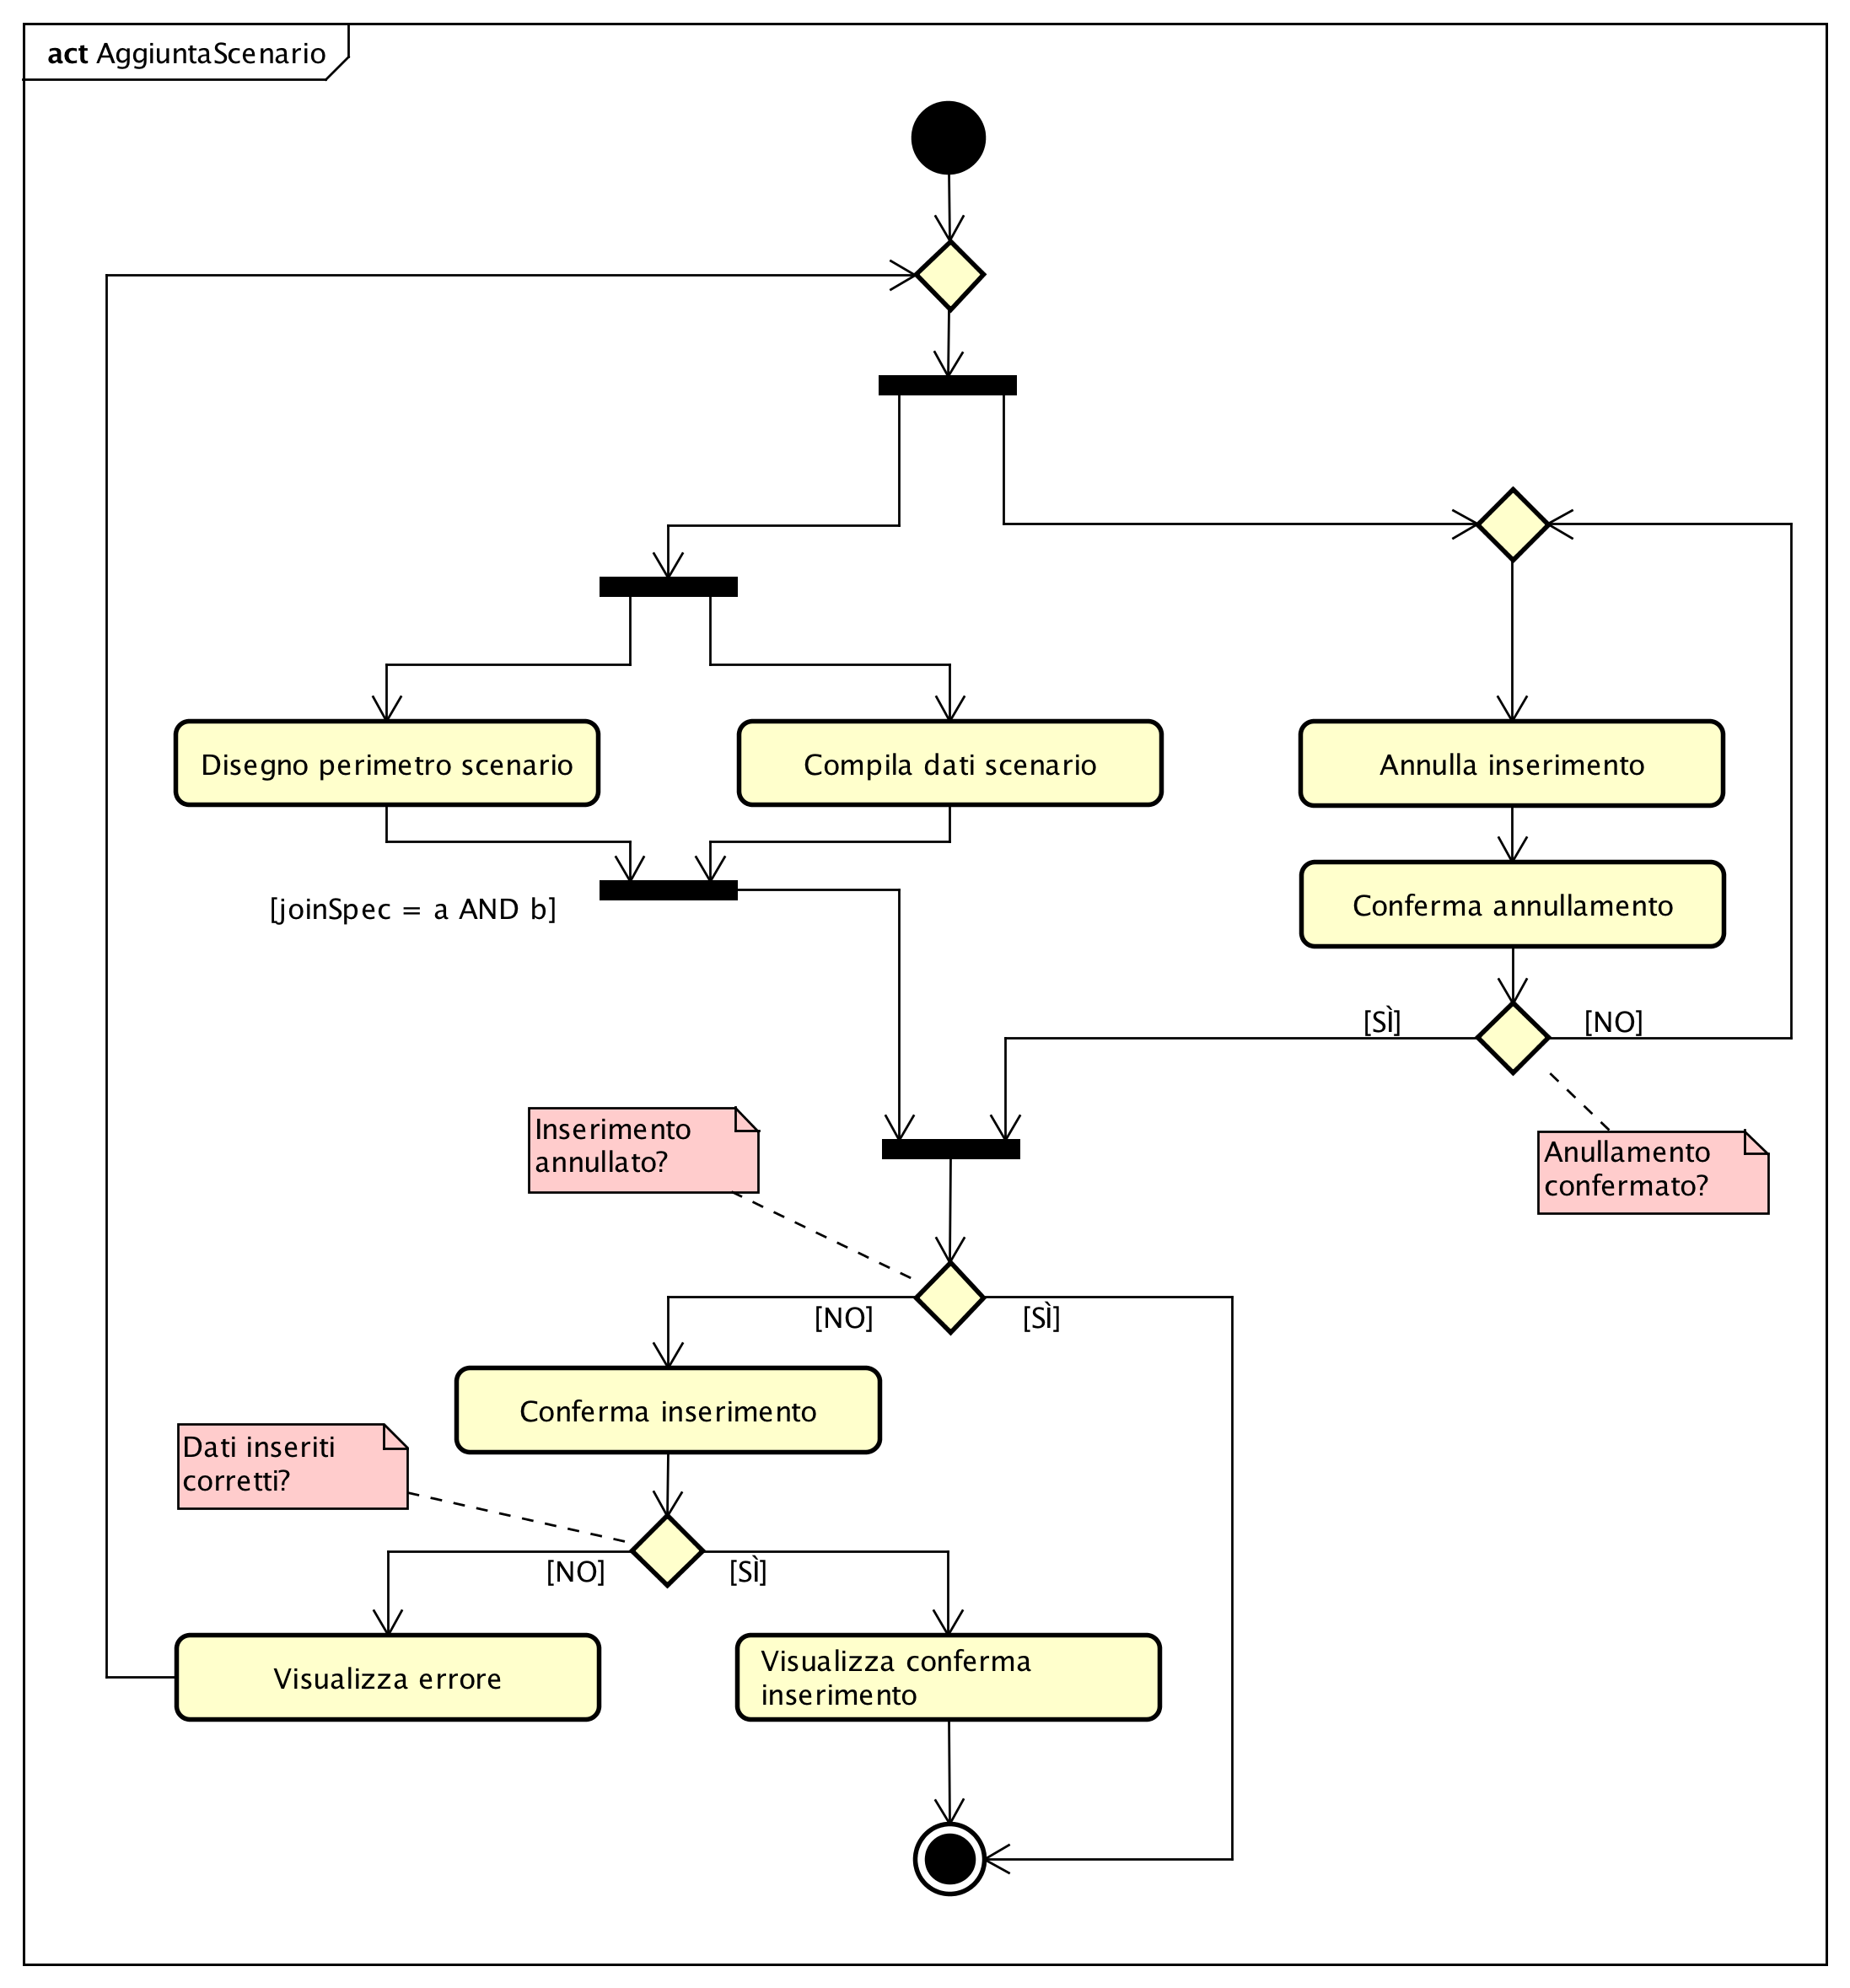
\includegraphics[width=\textwidth]{img/DiagrammiDiAttivita/AggiuntaScenario.png}
	\caption{Diagramma di attività per l'aggiunta di uno scenario}
\end{figure}
\begin{figure}[H]
	\centering
	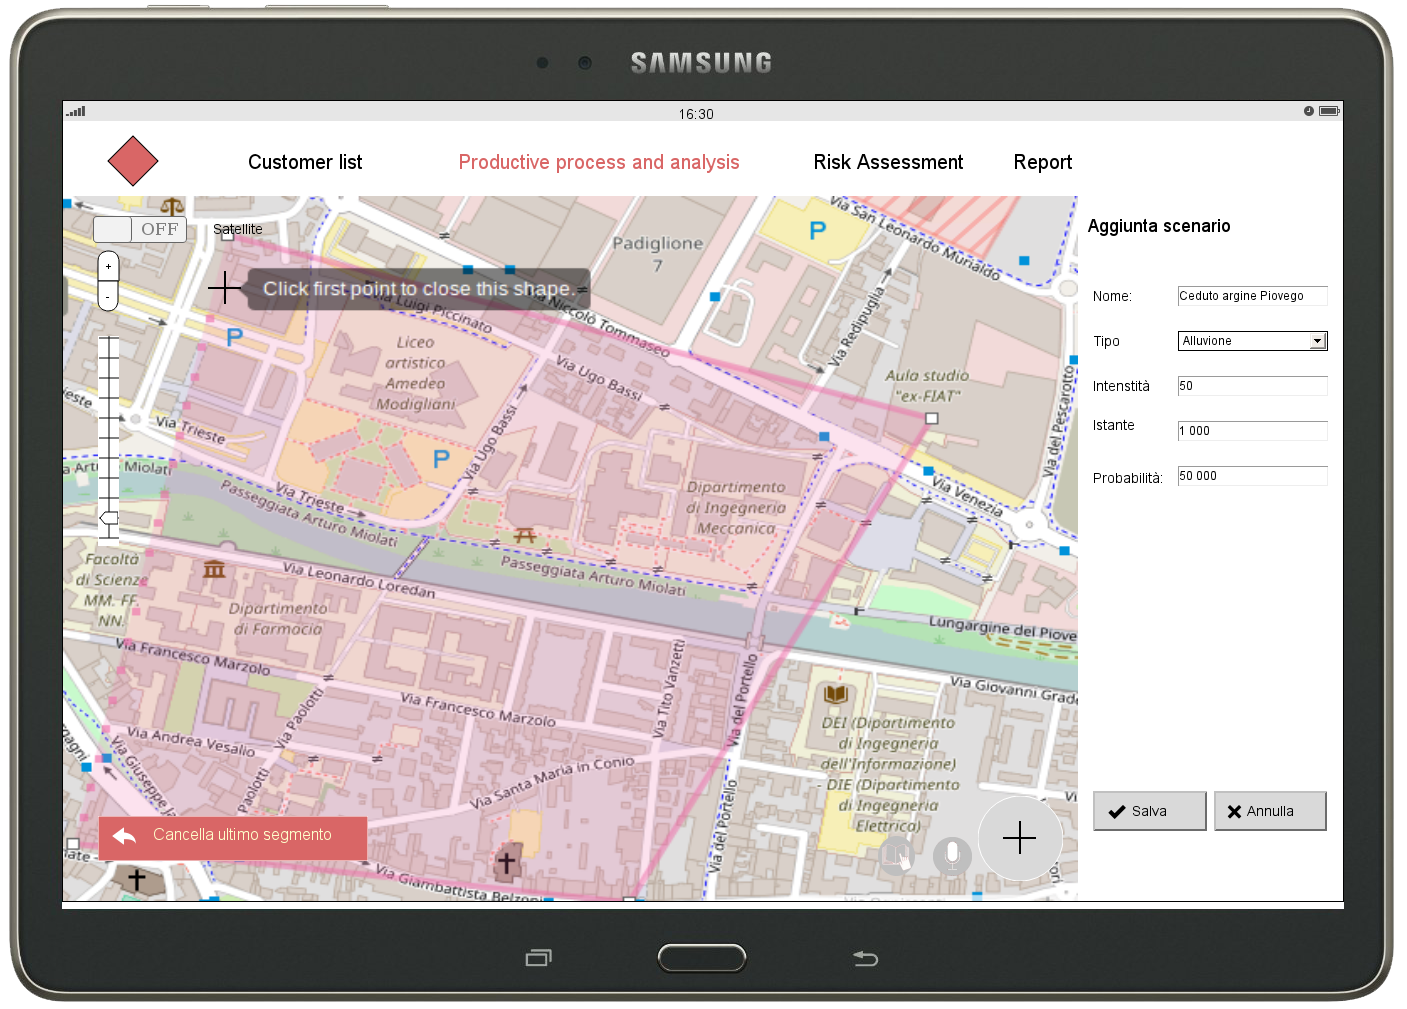
\includegraphics[width=\textwidth]{img/MockUp/m20.png}
	\caption{Mockup per l'aggiunta di uno scenario}
\end{figure}

\newpage
\subsection{Gestione Analisi}
Dopo essere entrati nella sezione di analisi, l'utente può effettuare ripetutamente una tra le seguenti operazioni:
\begin{itemize}
	\item è possibile aggiungere scenari su cui non è ancora stata calcolata alla lista di quelli da analizzare. In seguito è possibile avviare l'analisi;
	\item è possibile eliminare scenari dalla lista degli scenari su cui è stata calcolata l'analisi. In questo caso l'utente è invitato a confermare l'eliminazione o ad annullarla;
	\item l'utente non può effettuare alcuna operazione all'interno della sezione di analisi, se non sono presenti scenari.
\end{itemize} 
\begin{figure}[H]
	\centering
	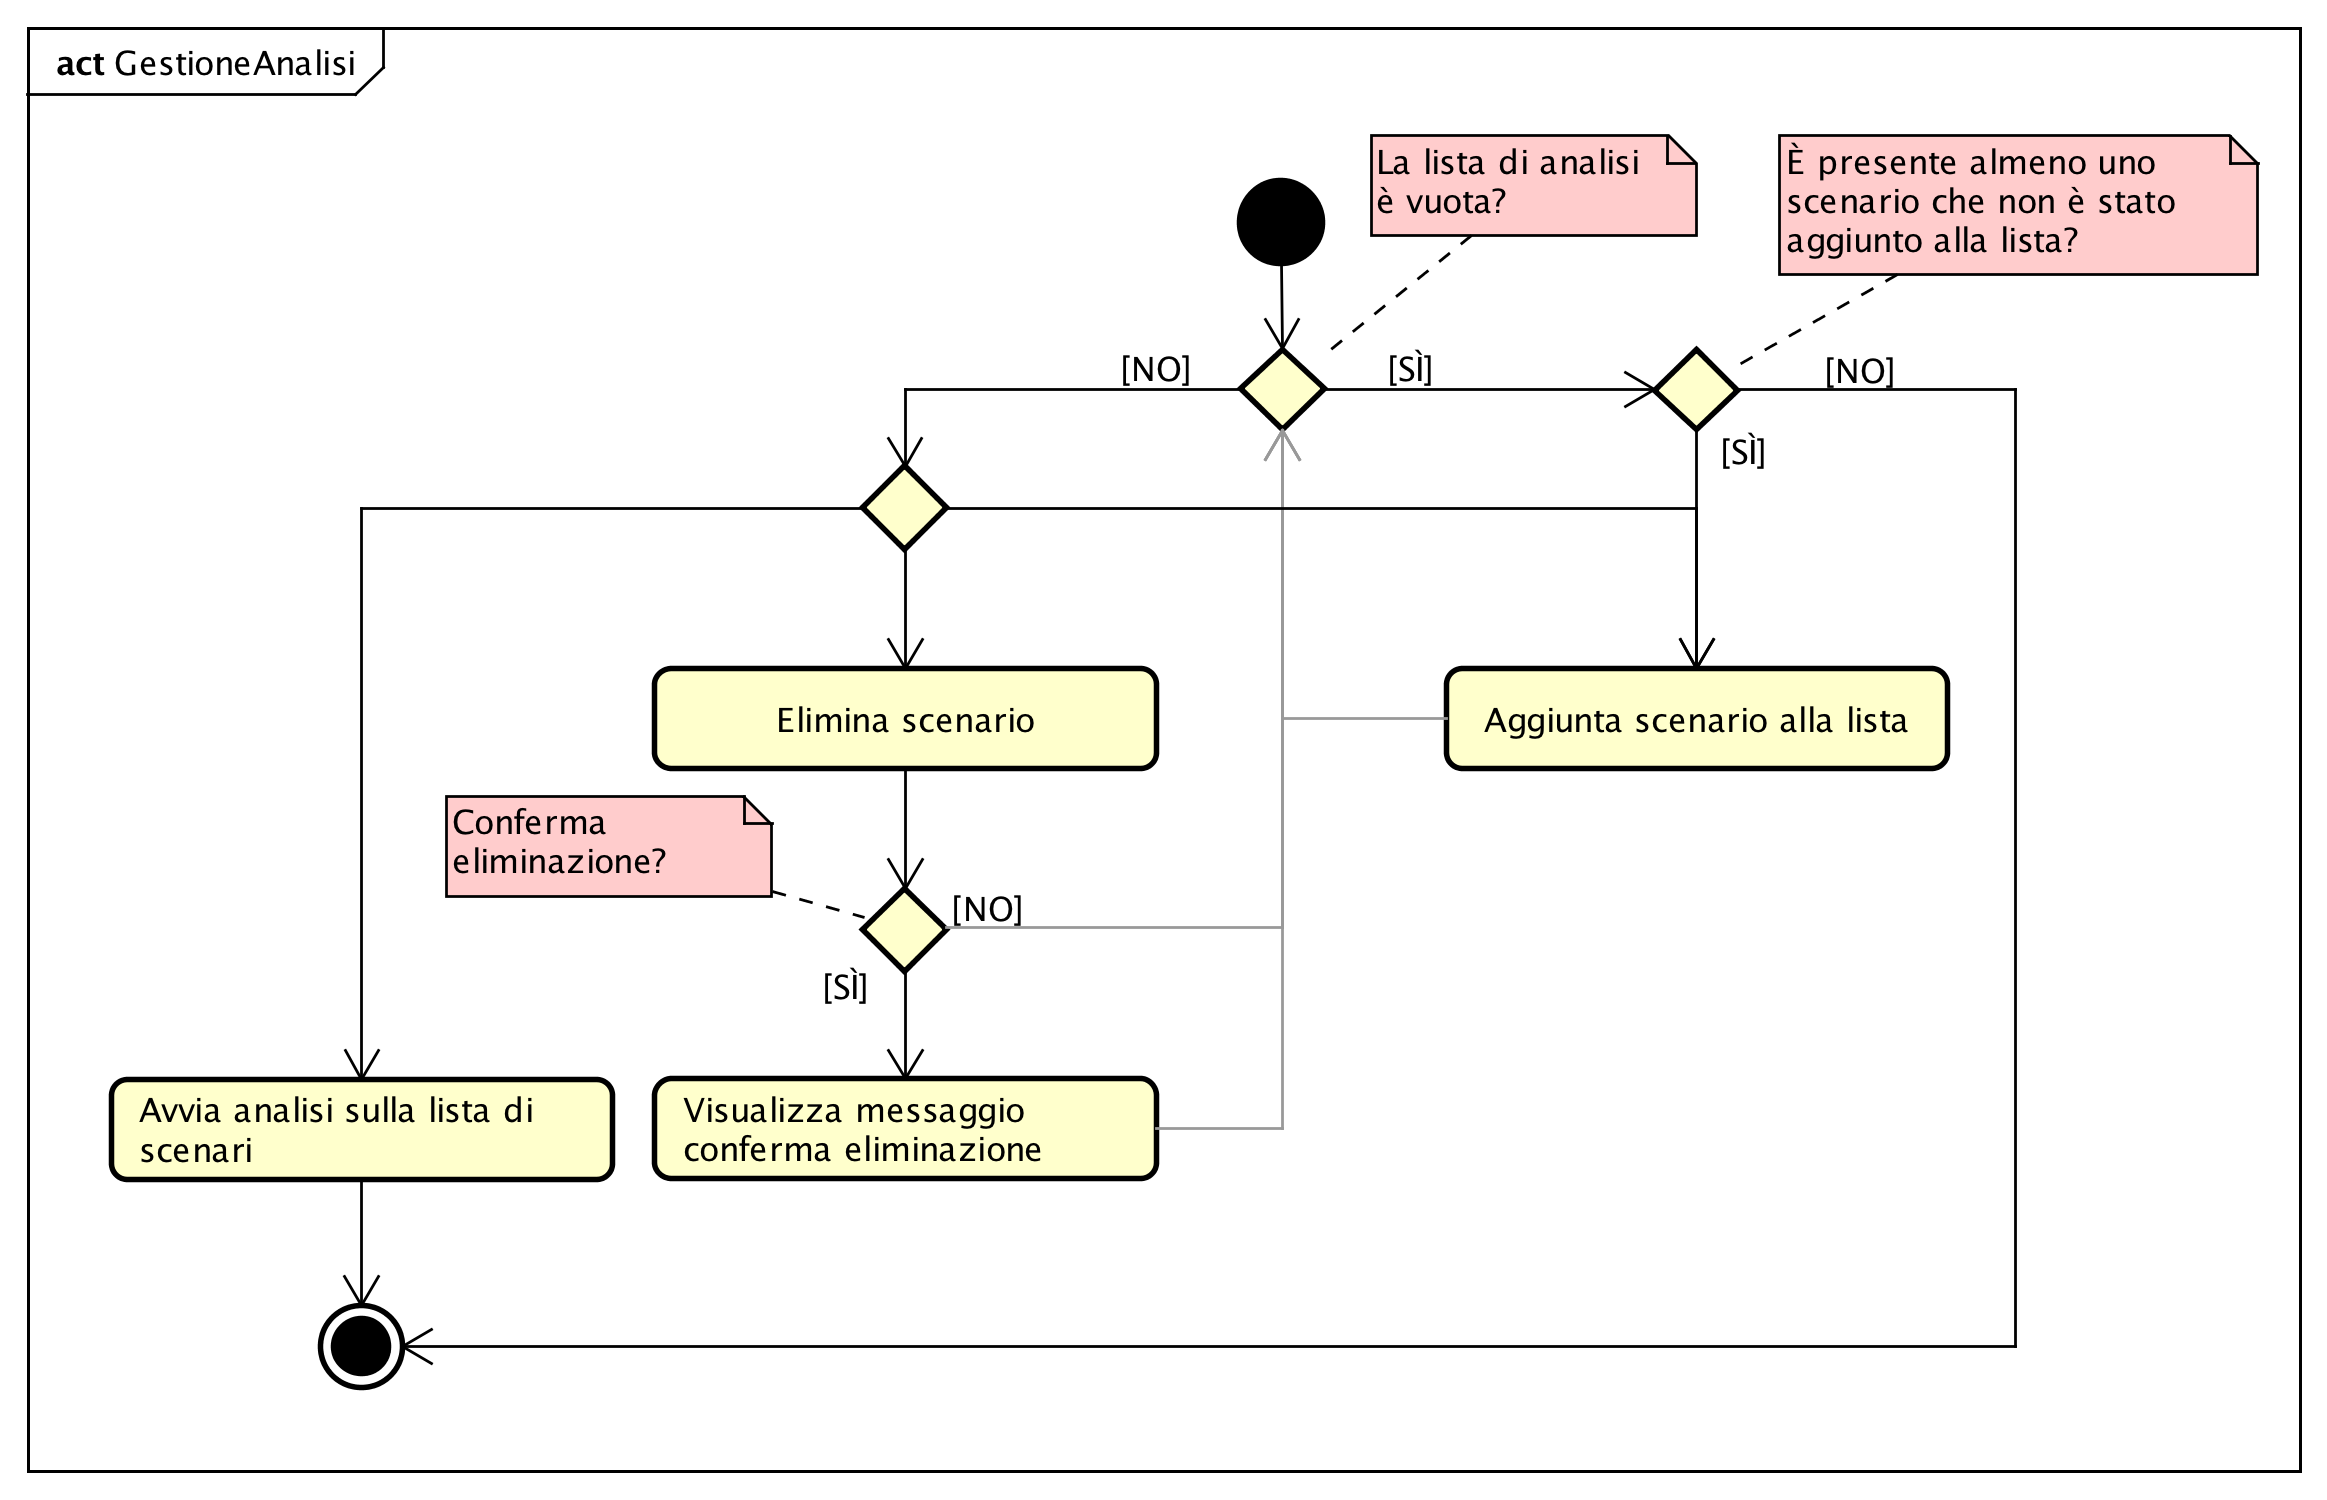
\includegraphics[width=\textwidth]{img/DiagrammiDiAttivita/GestioneAnalisi.png}
	\caption{Diagramma di attività per la gestione analisi}
\end{figure}
\begin{figure}[H]
	\centering
	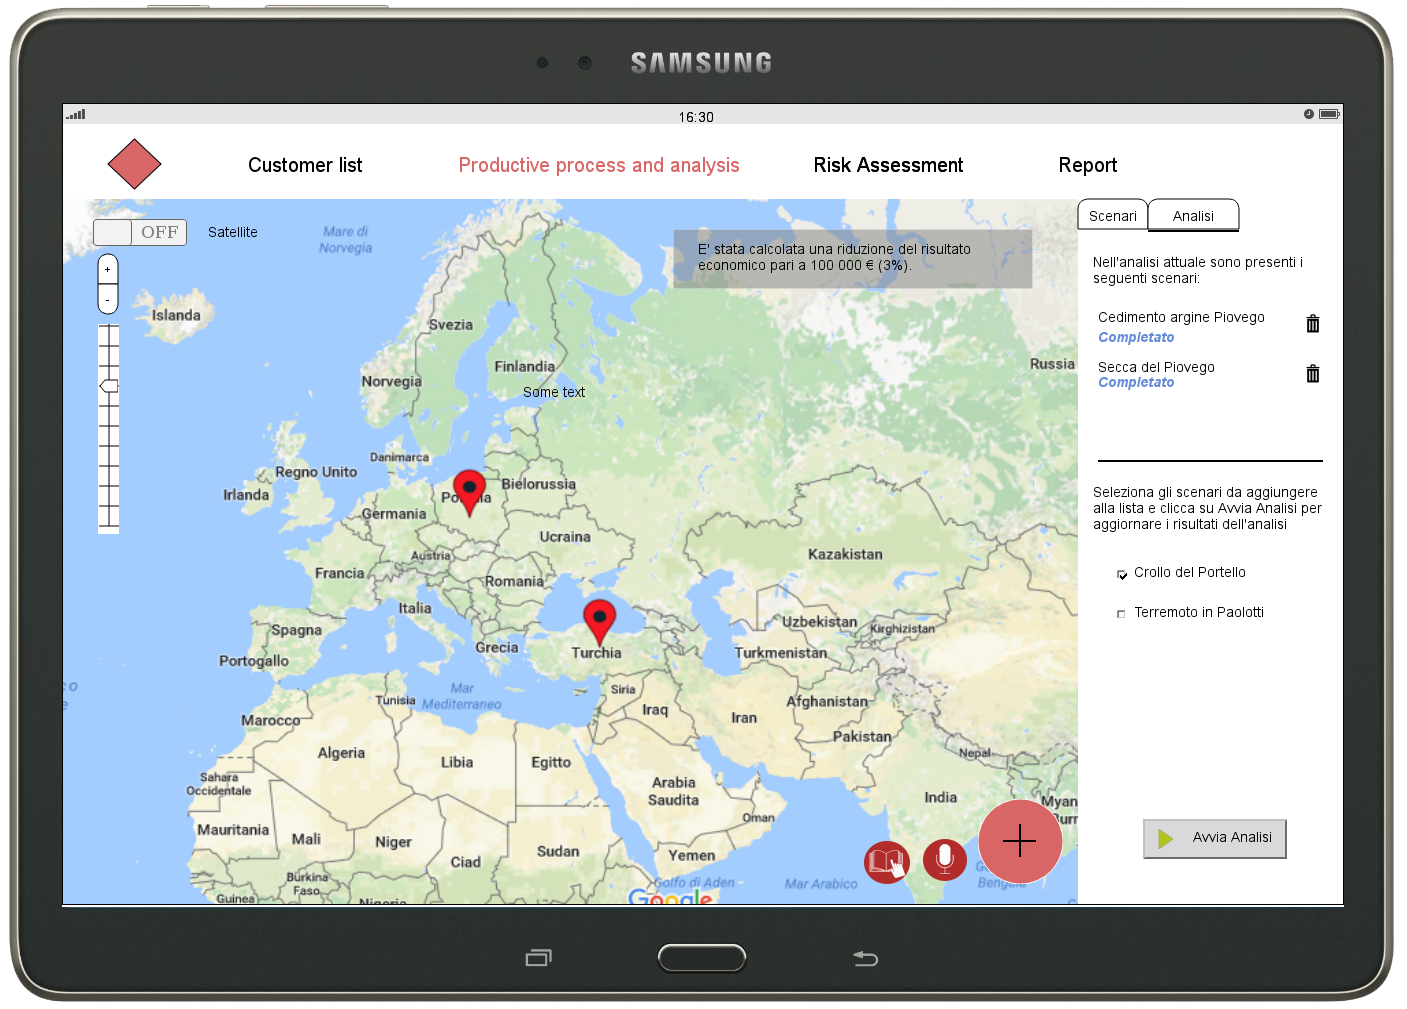
\includegraphics[scale=0.29]{img/MockUp/m2.png}
	\caption{Mockup per l'avvio dell'analisi}
\end{figure}
\begin{figure}[H]
	\centering
	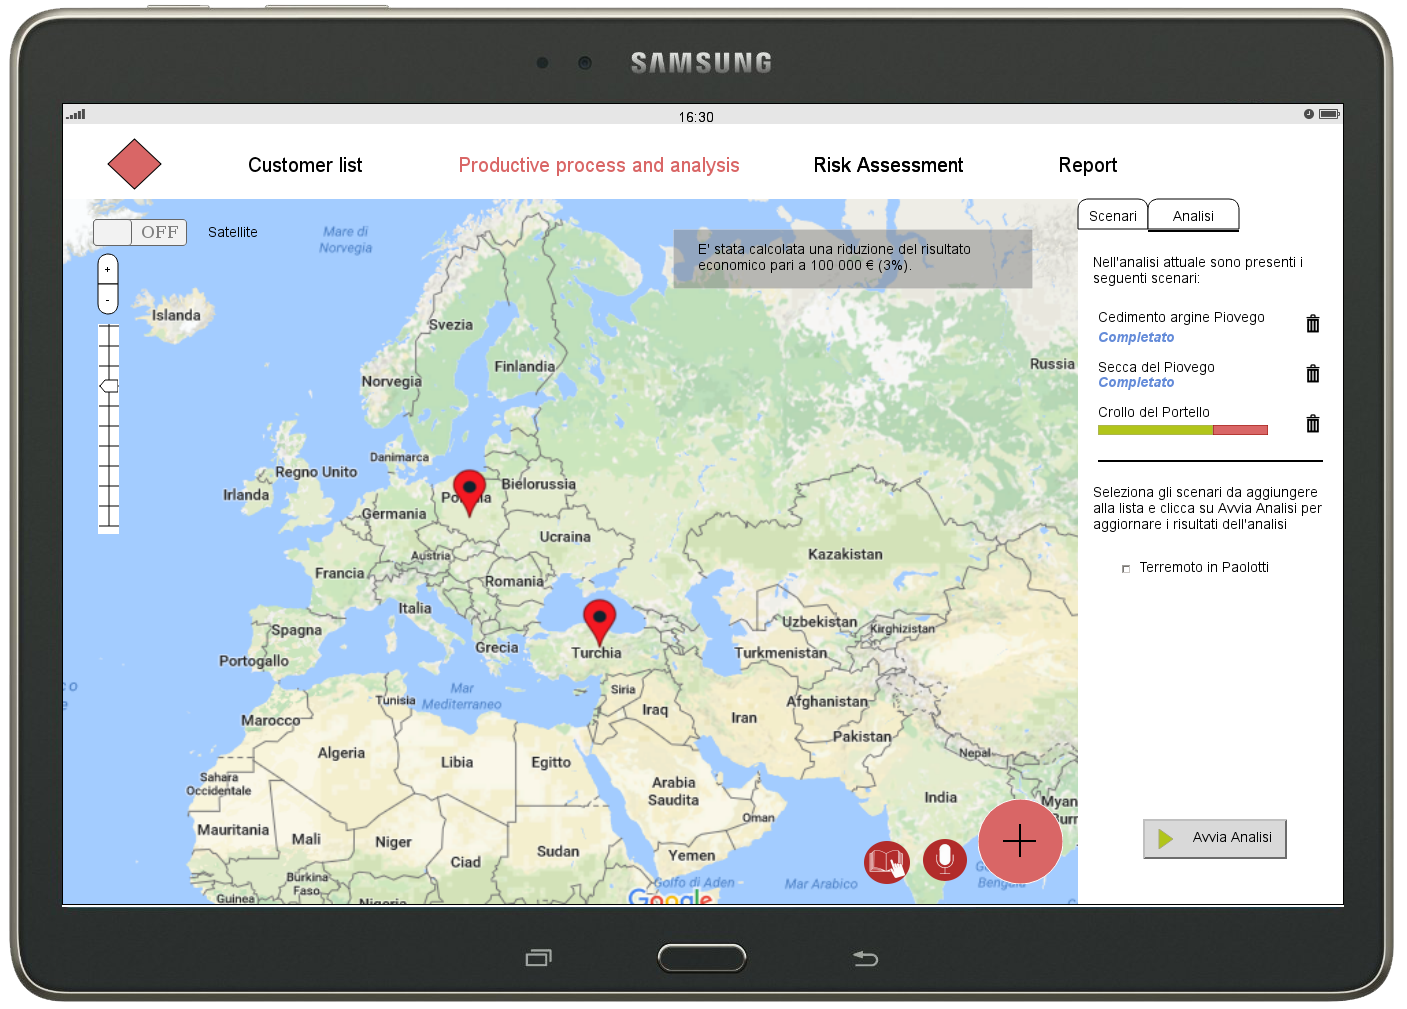
\includegraphics[scale=0.29]{img/MockUp/m3.png}
	\caption{Mockup per l'analisi in corso}
\end{figure}


\newpage
\subsection{Selezione asset}
Una volta selezionato l'asset l'utente potrà:
\begin{itemize}
	\item centrarlo automaticamente sulla mappa (utile nel caso in cui nel frattempo l'utente si sia spostato sulla mappa), eventualmente più volte, senza annullarne la selezione;
	\item annullarne la selezione;
	\item modificarlo;
	\item eliminarlo.
\end{itemize}
\begin{figure}[H]
	\centering
	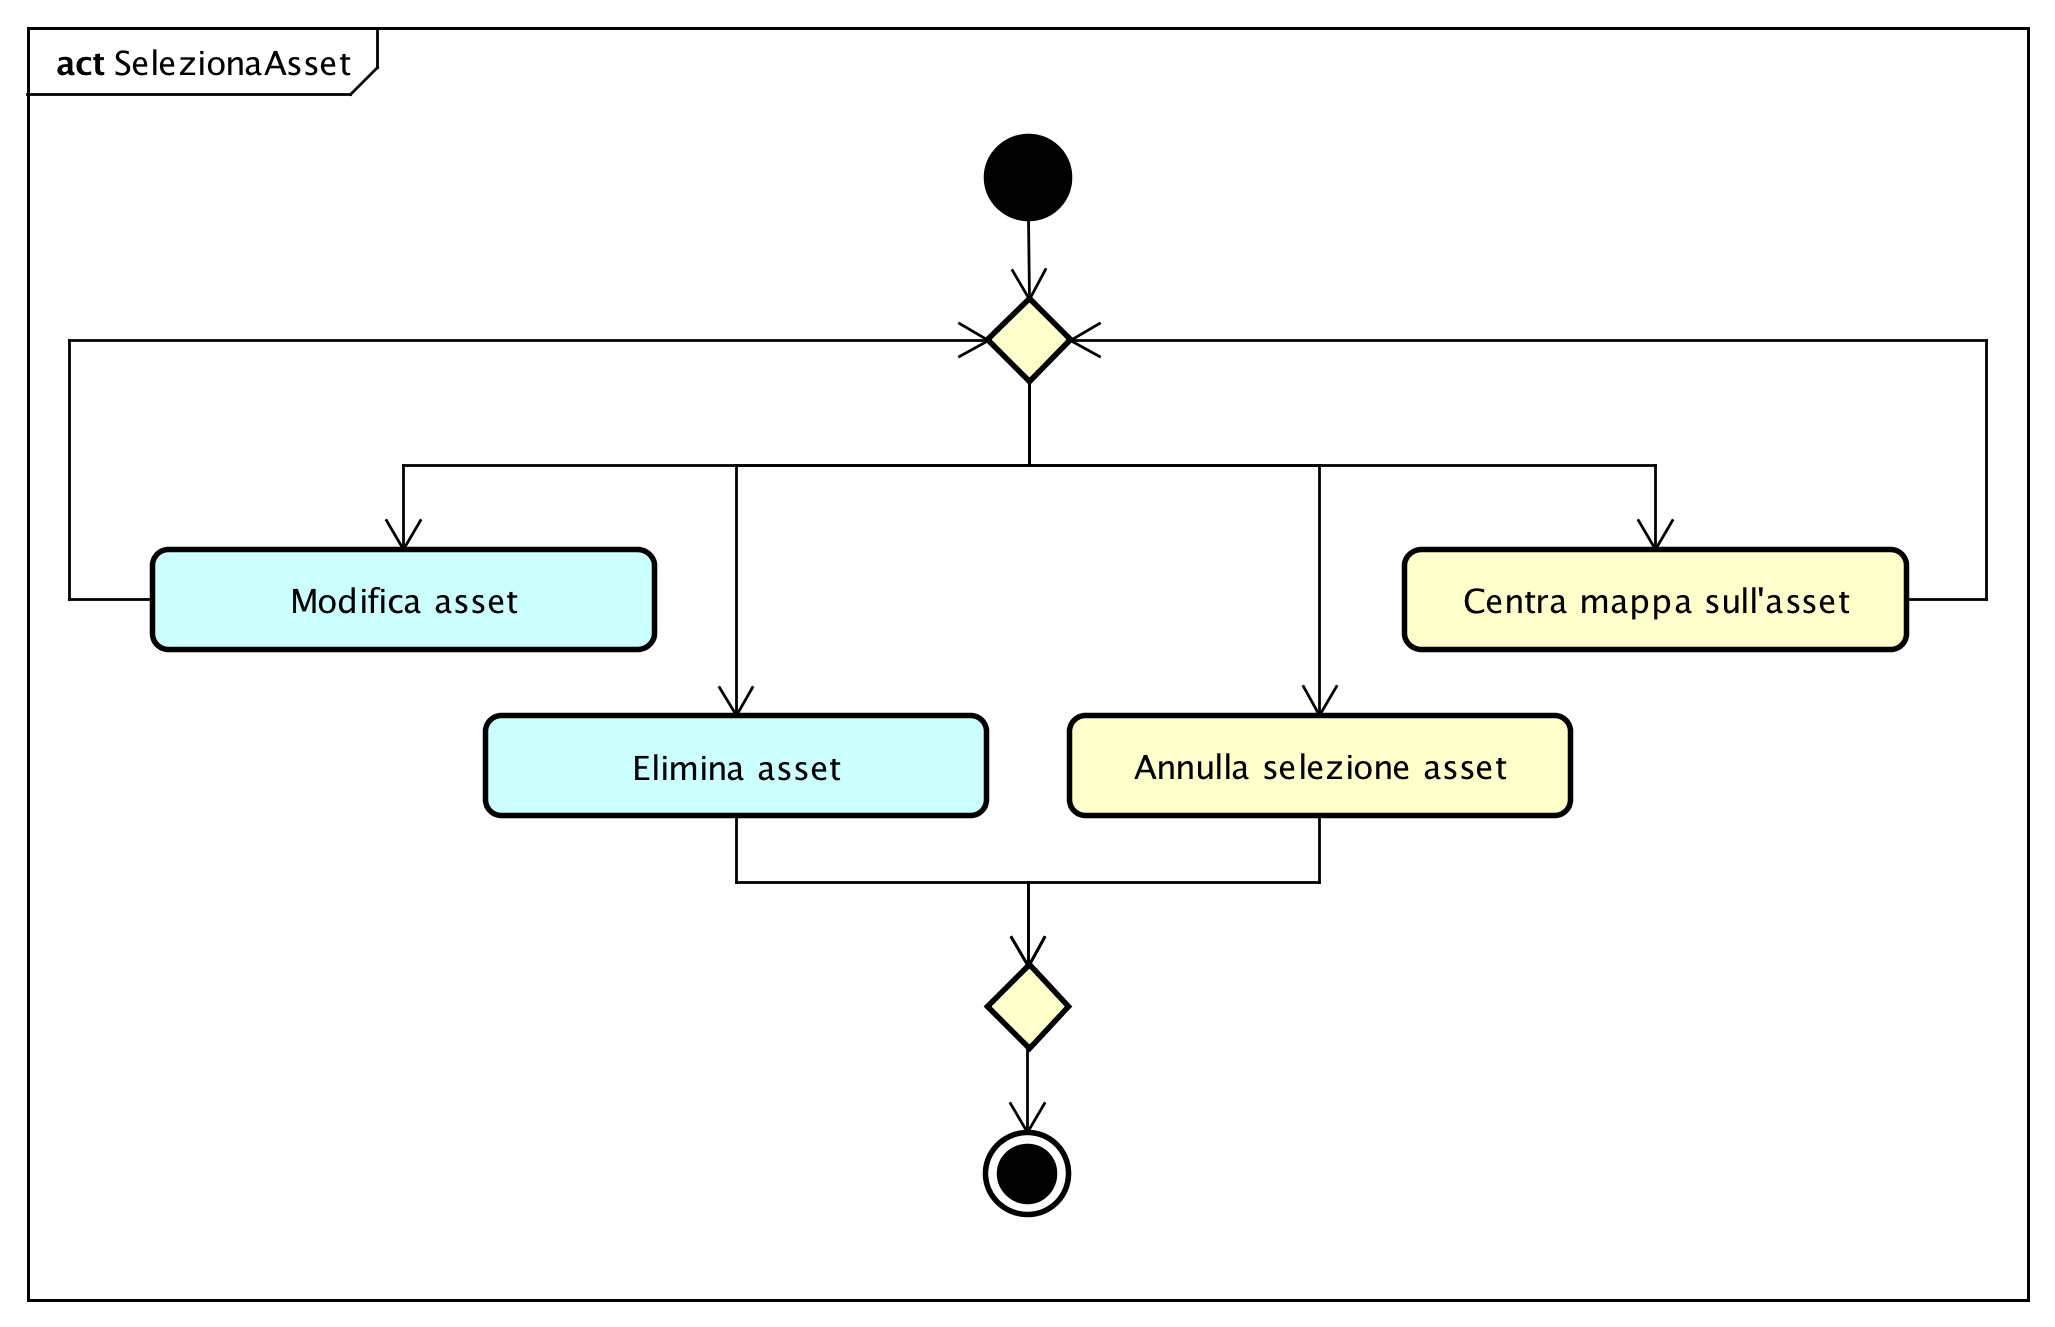
\includegraphics[width=\textwidth]{img/DiagrammiDiAttivita/SelezioneAsset.png}
	\caption{Diagramma di attività per la selezione di un asset}
\end{figure}
\label{7_Visualizza_un_asset}
\begin{figure}[H]
	\centering
	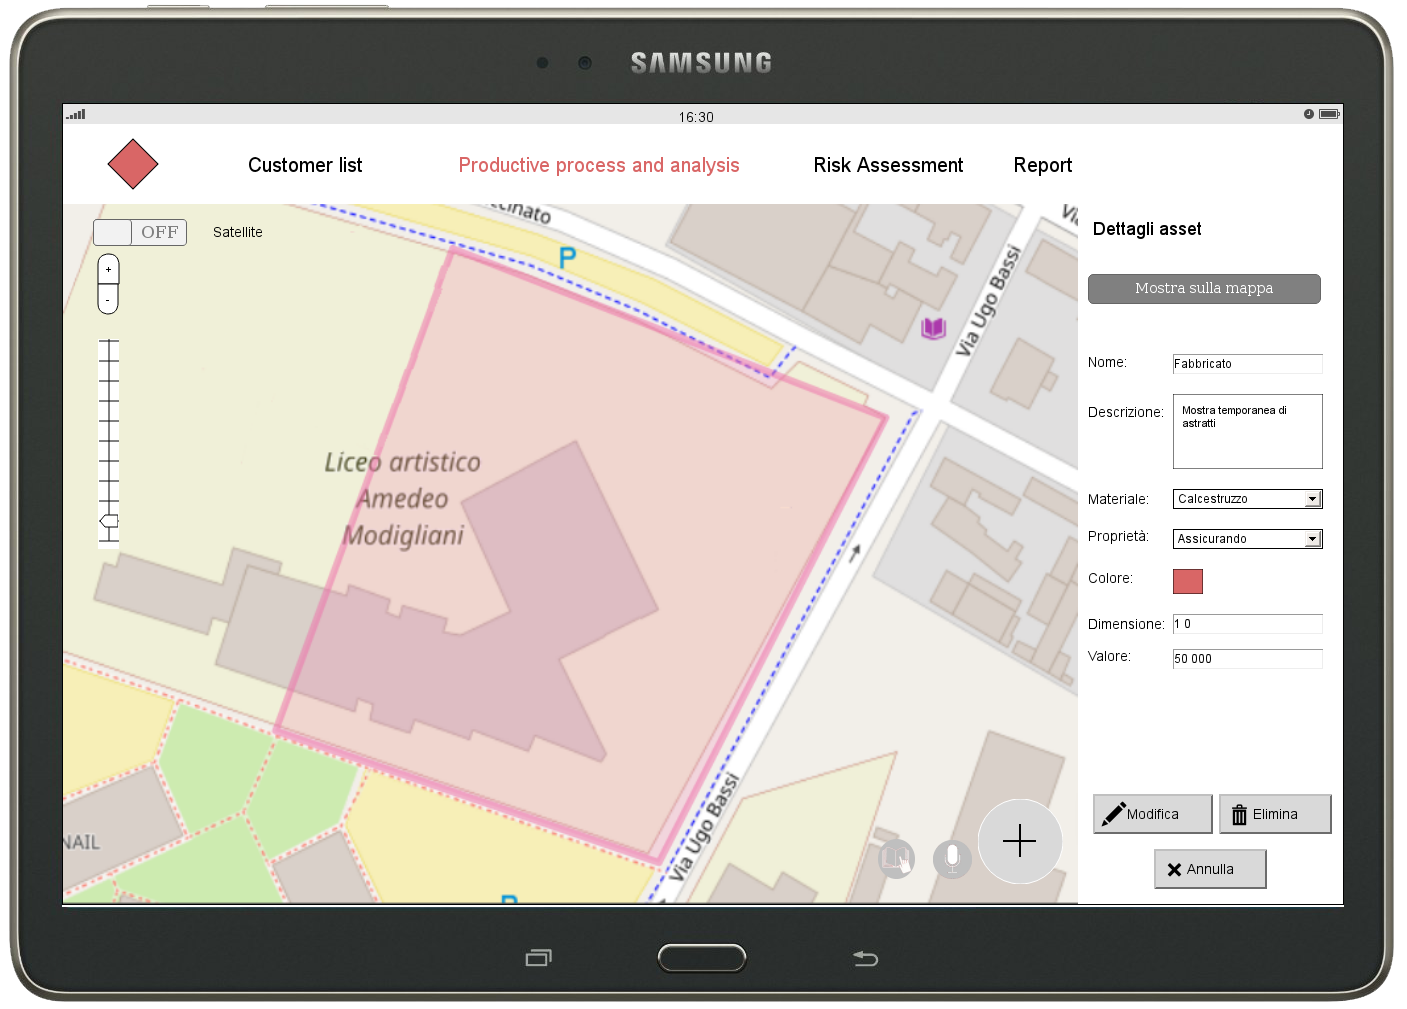
\includegraphics[width=\textwidth]{img/MockUp/m7.png}
	\caption{Mockup per la selezione di un asset}
\end{figure}

\newpage
\subsection{Selezione nodo}
Una volta selezionato il nodo l'utente potrà:
\begin{itemize}
	\item centrarlo automaticamente sulla mappa (utile nel caso in cui nel frattempo l'utente si sia spostato sulla mappa), eventualmente più volte, senza annullarne la selezione;
	\item annullarne la selezione;
	\item modificarlo;
	\item eliminarlo.
\end{itemize}
\begin{figure}[H]
	\centering
	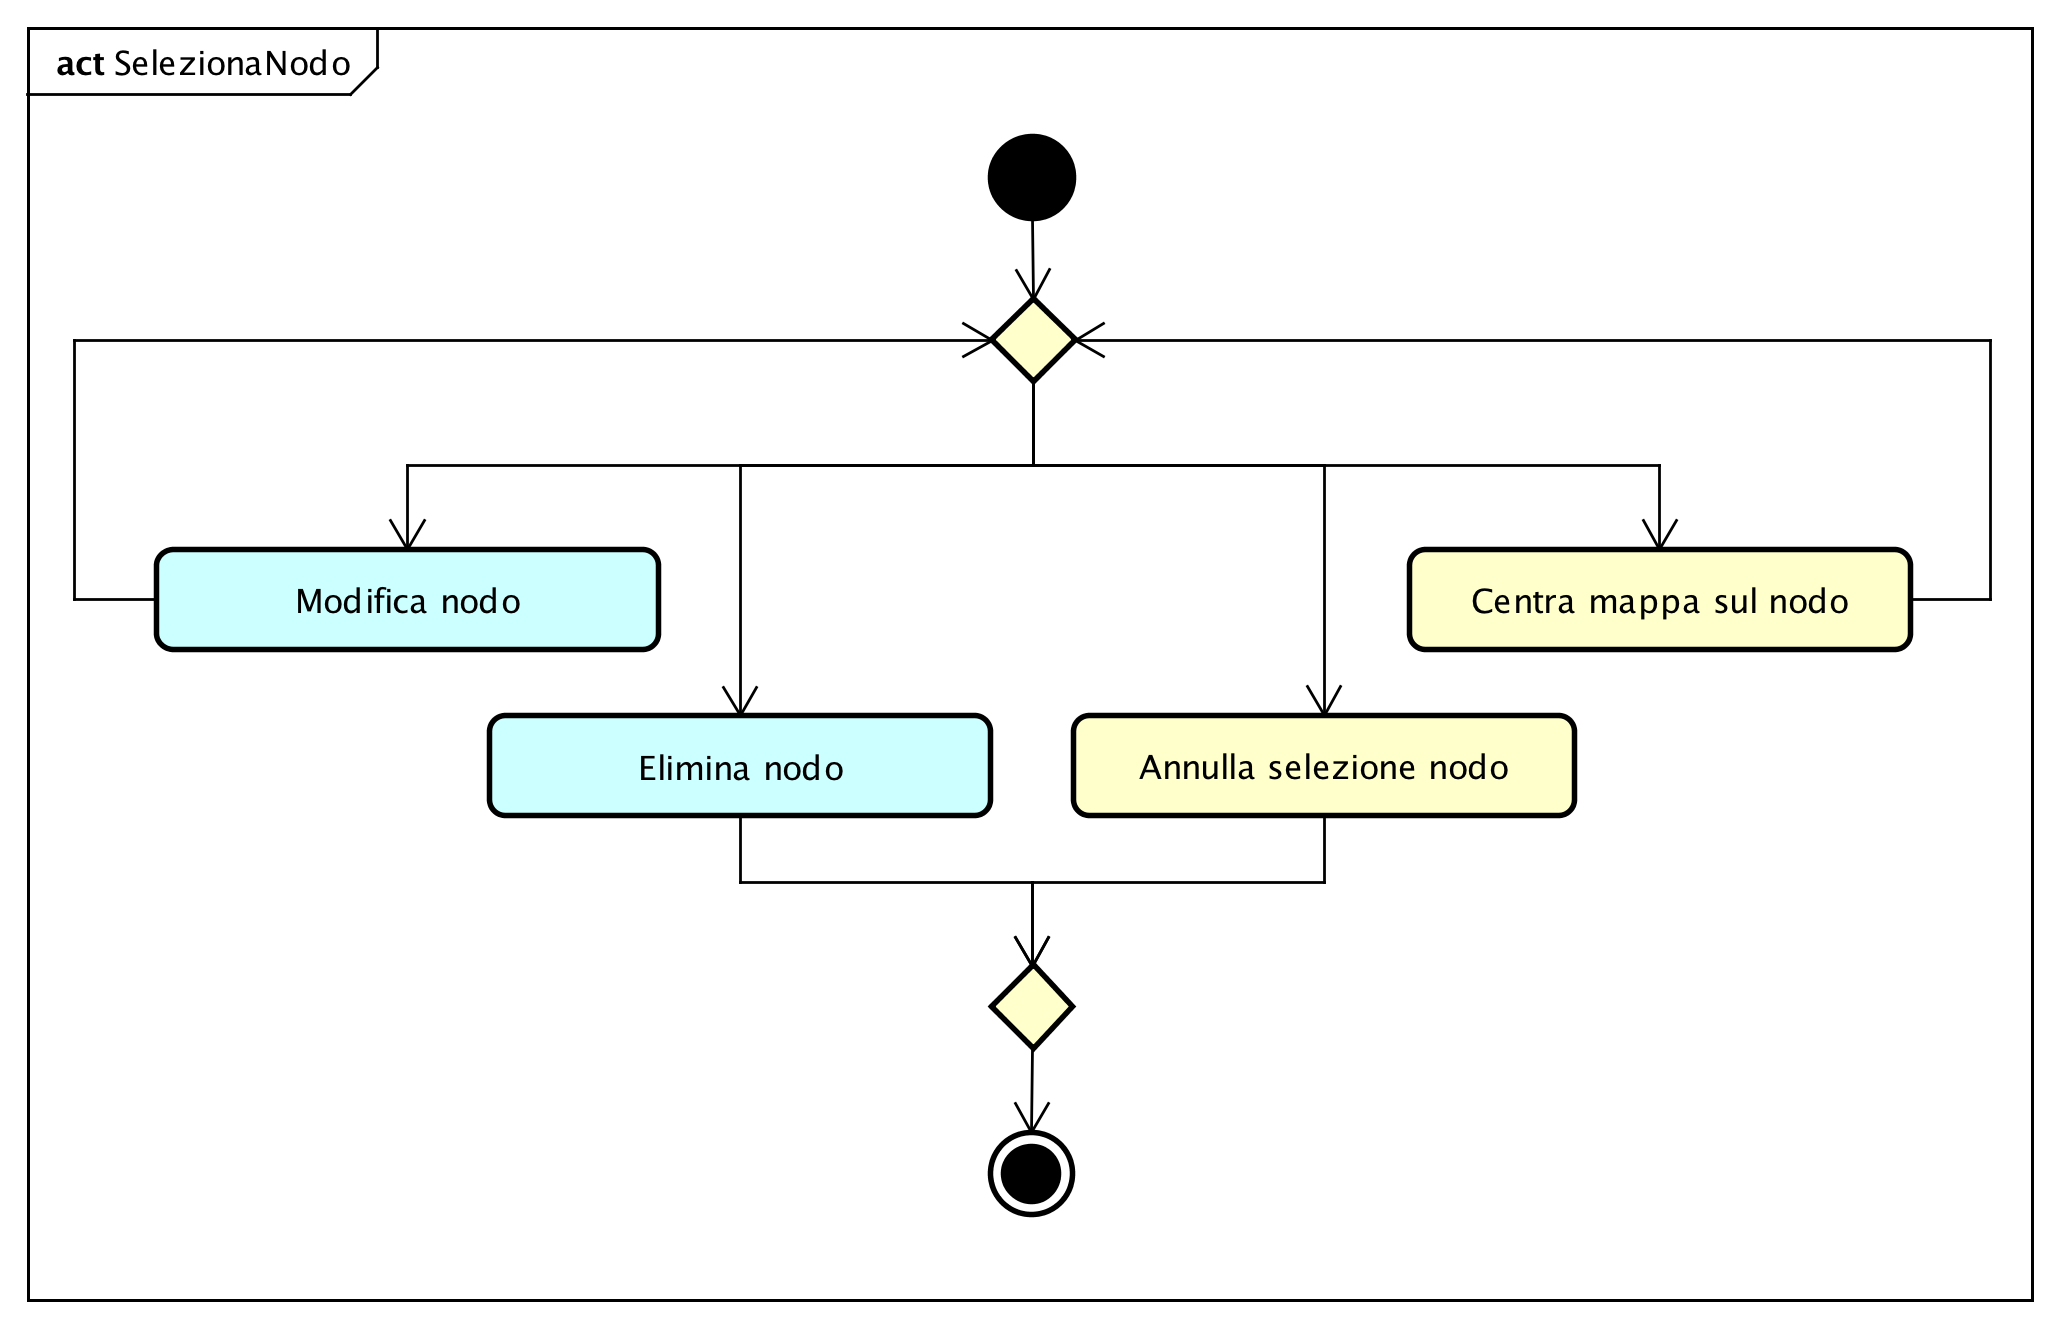
\includegraphics[width=\textwidth]{img/DiagrammiDiAttivita/SelezioneNodo.png}
	\caption{Diagramma di attività per la selezione di un nodo}
\end{figure}
\begin{figure}[H]
	\centering
	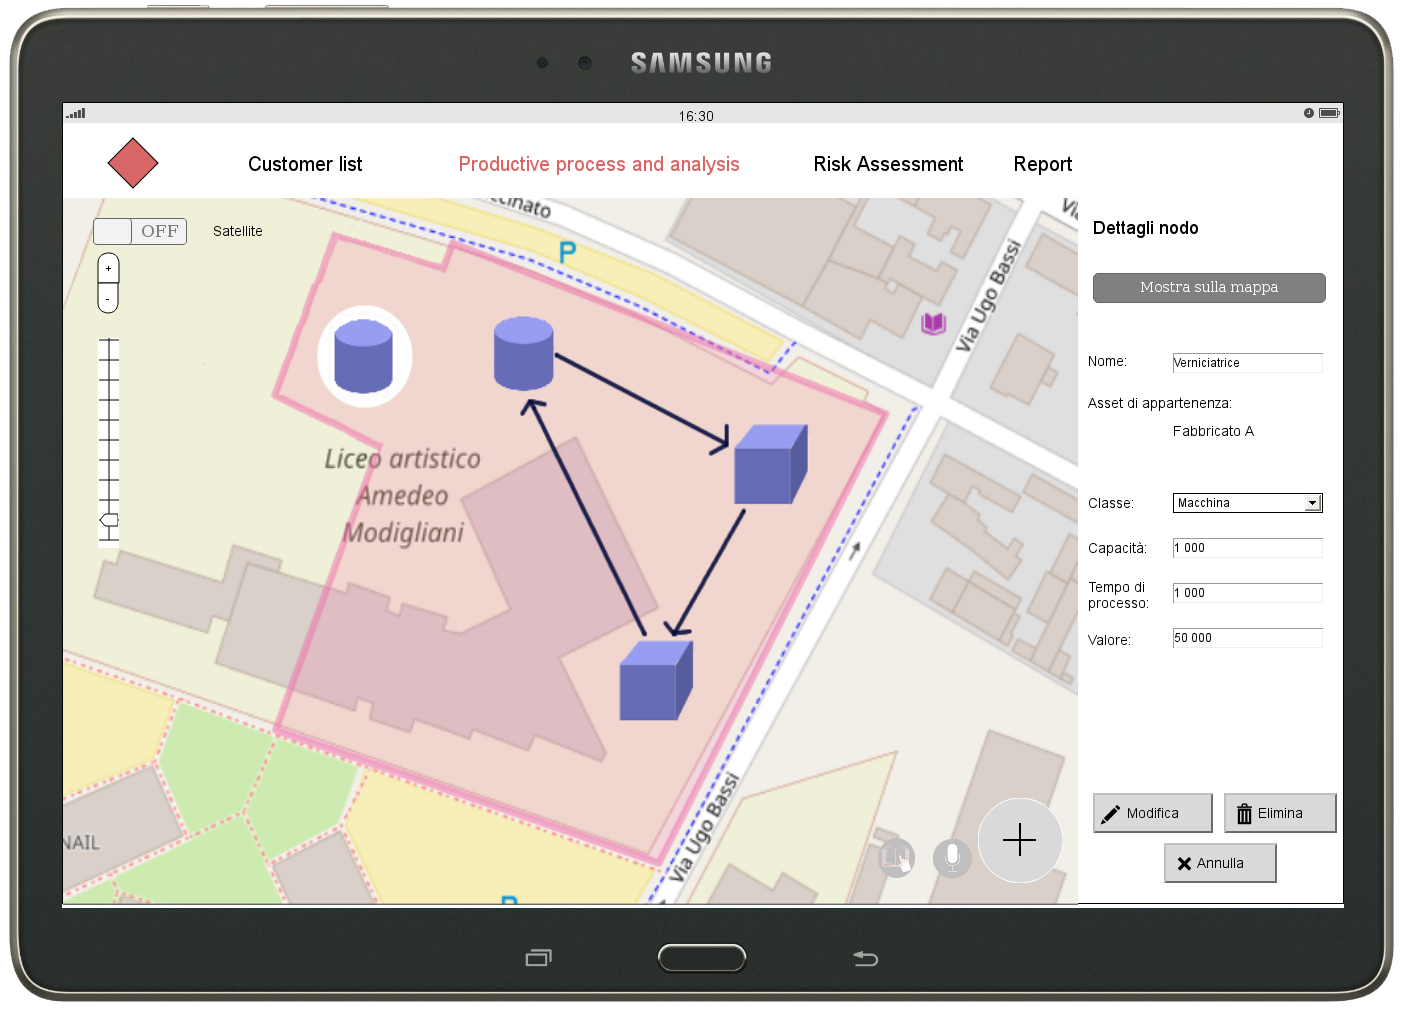
\includegraphics[width=\textwidth]{img/MockUp/m13.png}
	\caption{Mockup per la selezione di un nodo}
\end{figure}

\newpage
\subsection{Selezione arco}
Una volta selezionato il nodo l'utente potrà:
\begin{itemize}
	\item centrarlo automaticamente sulla mappa (utile nel caso in cui nel frattempo l'utente si sia spostato sulla mappa), eventualmente più volte, senza annullarne la selezione;
	\item annullarne la selezione;
	\item modificarlo;
	\item eliminarlo.
\end{itemize}
\begin{figure}[H]
	\centering
	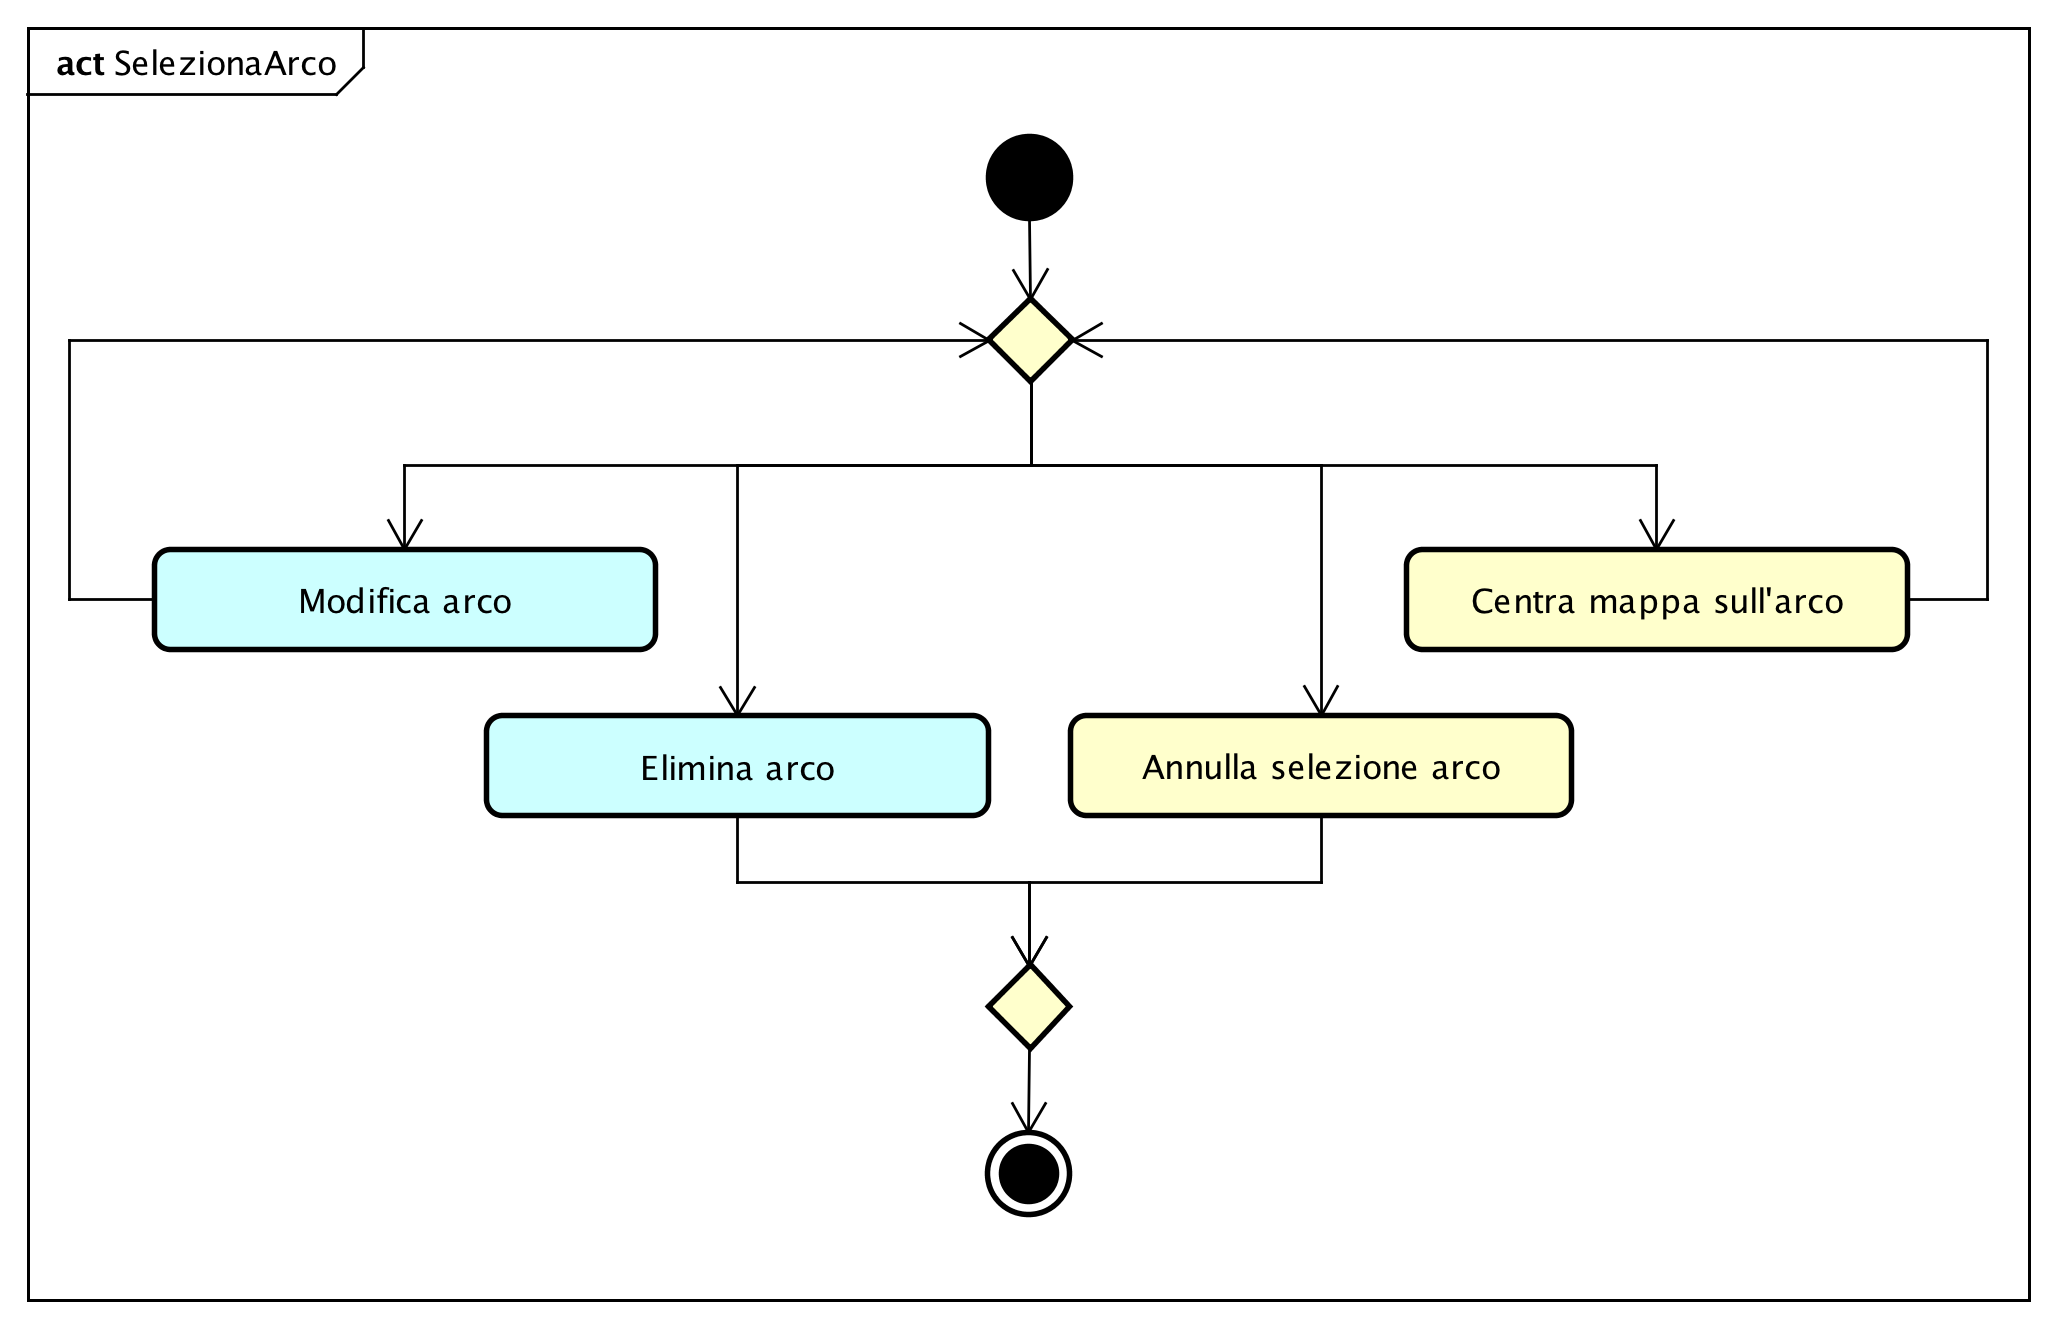
\includegraphics[width=\textwidth]{img/DiagrammiDiAttivita/SelezioneArco.png}
	\caption{Diagramma di attività per la selezione di un arco}
\end{figure}

\newpage
\subsection{Selezione scenario}
Una volta selezionato lo scenario l'utente potrà:
\begin{itemize}
	\item annullarne la selezione;
	\item selezionare un altro scenario;
	\item modificarlo;
	\item eliminarlo.
\end{itemize}
\begin{figure}[H]
	\centering
	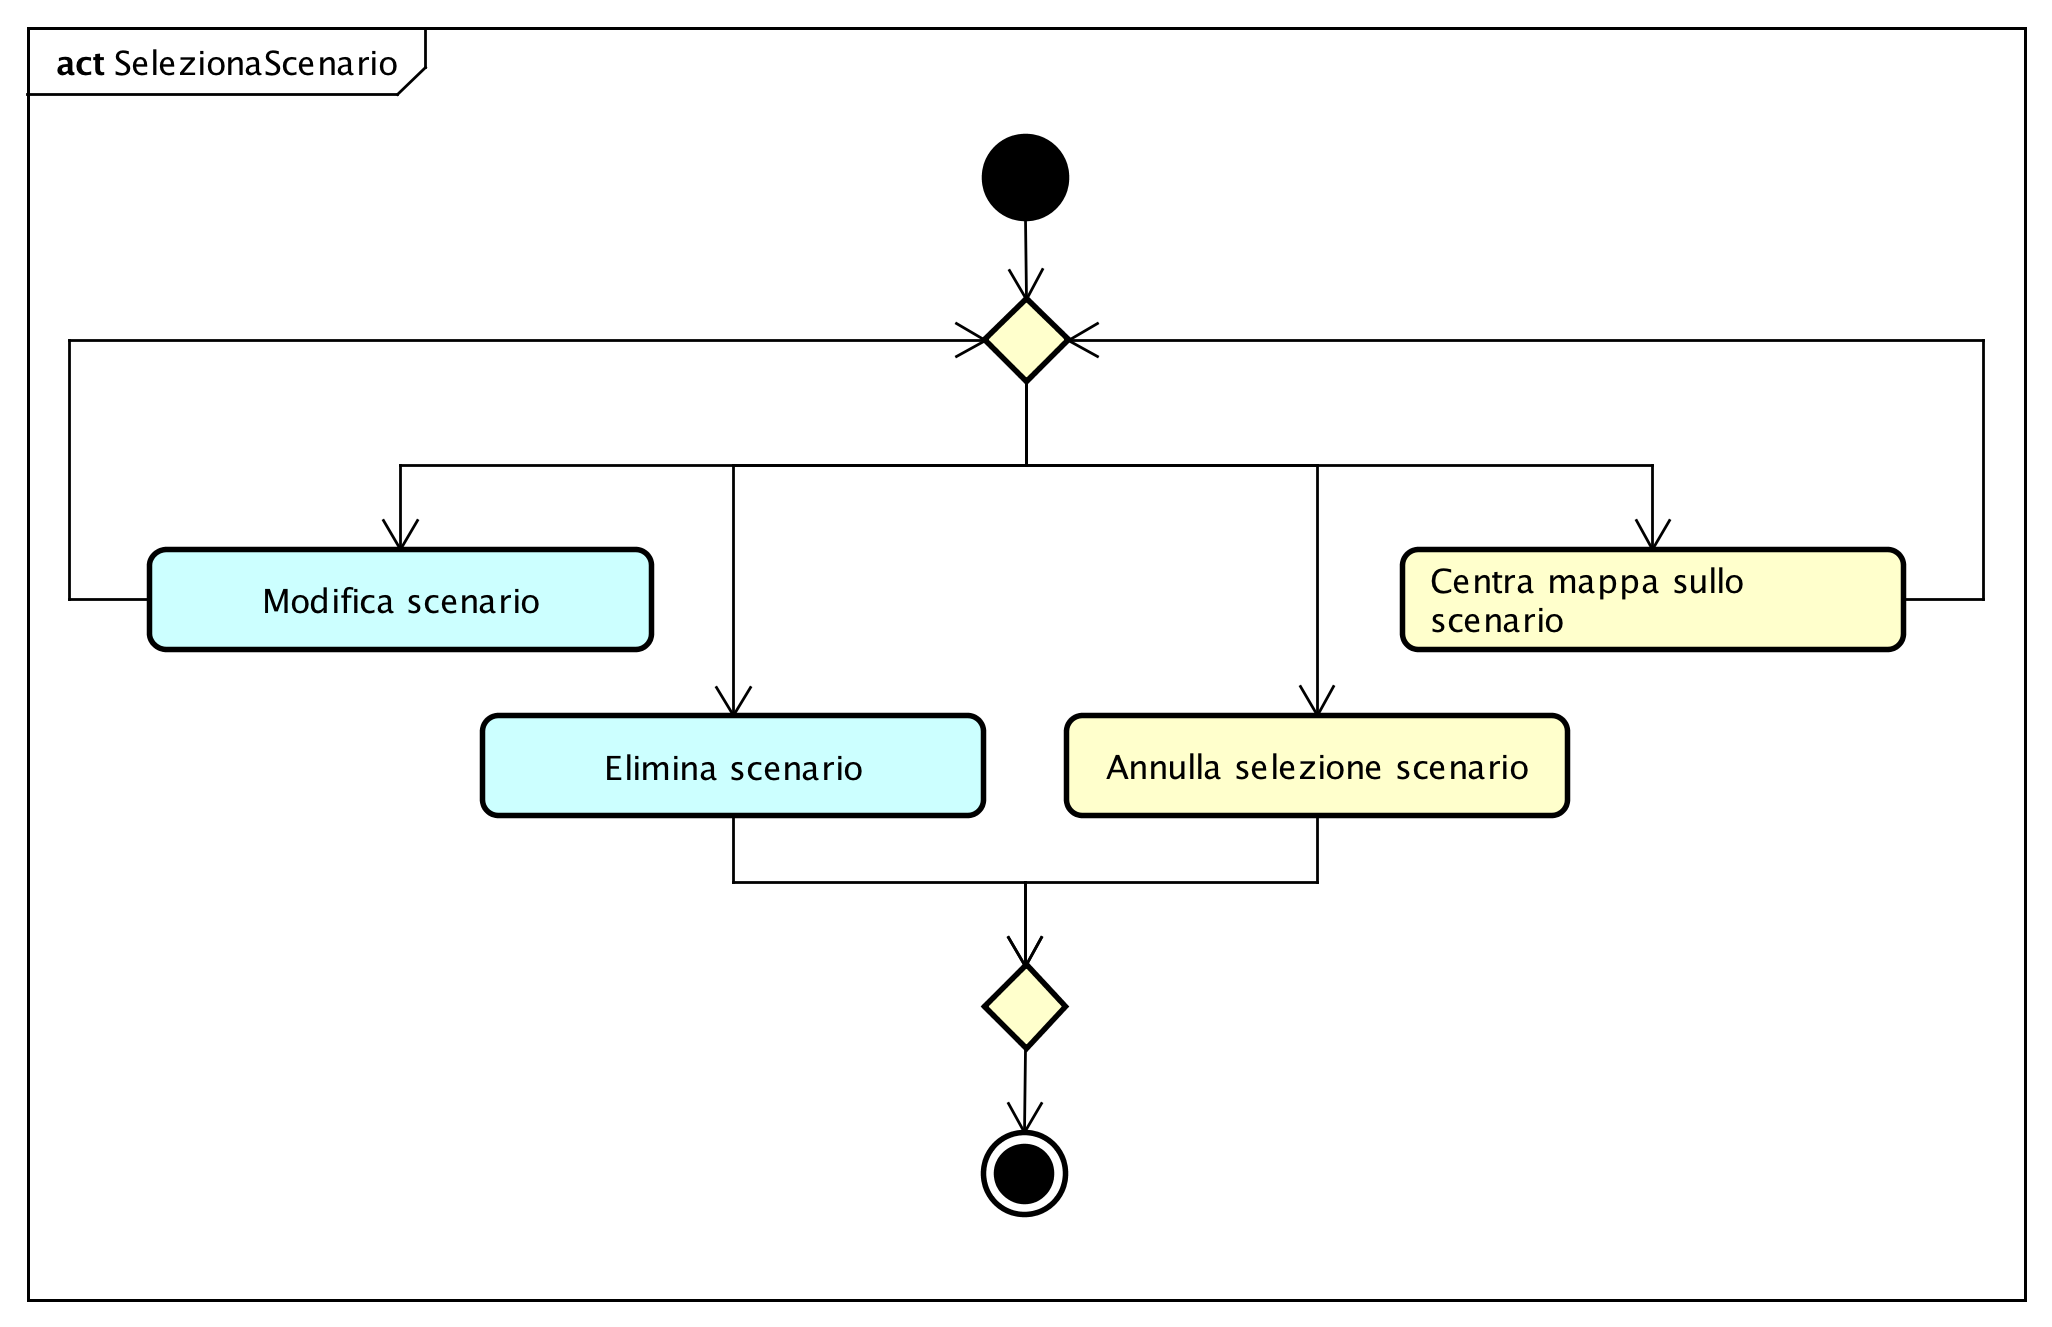
\includegraphics[width=\textwidth]{img/DiagrammiDiAttivita/SelezioneScenario.png}
	\caption{Diagramma di attività per la selezione di uno scenario}
\end{figure}
\begin{figure}[H]
	\centering
	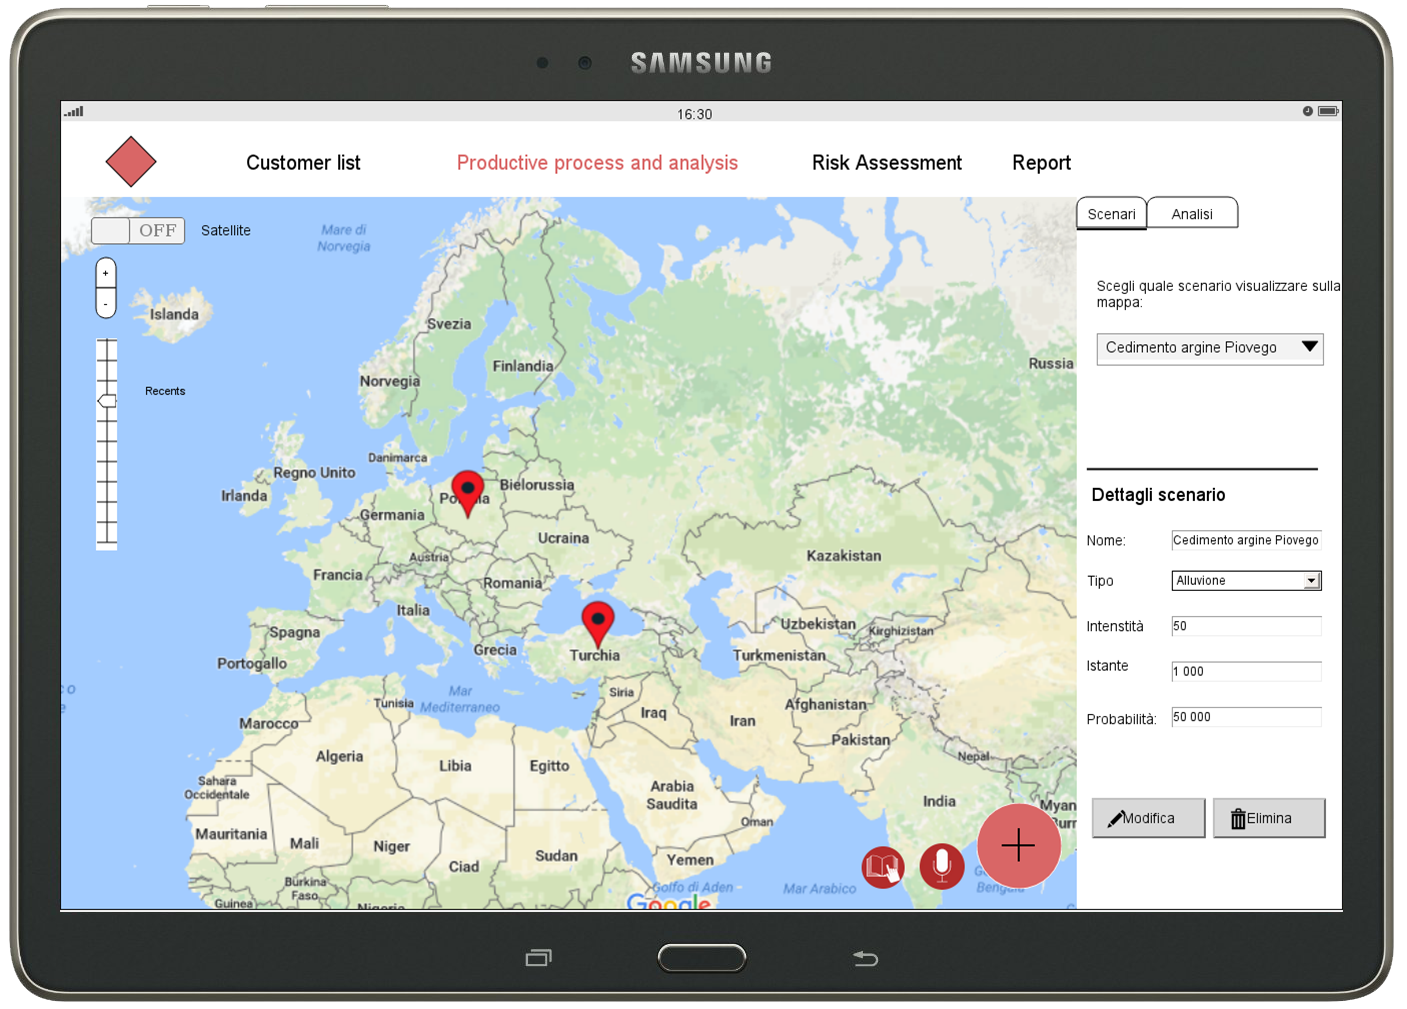
\includegraphics[width=\textwidth]{img/MockUp/m1.png}
	\caption{Mockup per la selezione di uno scenario}
\end{figure}

\newpage
\subsection{Modifica asset}
Per quanto riguarda la modifica dell'asset, sarà possibile ridisegnarne il perimetro dell'asset sulla mappa e/o modificarne i dati precedentemente compilati. Infine si dovrà confermare la modifica. In caso di dati non corretti, la modifica potrebbe non andare a buon fine: verrà visualizzato un messaggio di errore e l'utente sarà tenuto a correggere eventuali errori o incompletezze.
In ogni momento l'utente può annullare la modifica. Il sistema richiede una conferma per portare a termine tale operazione.
\begin{figure}[H]
	\centering
	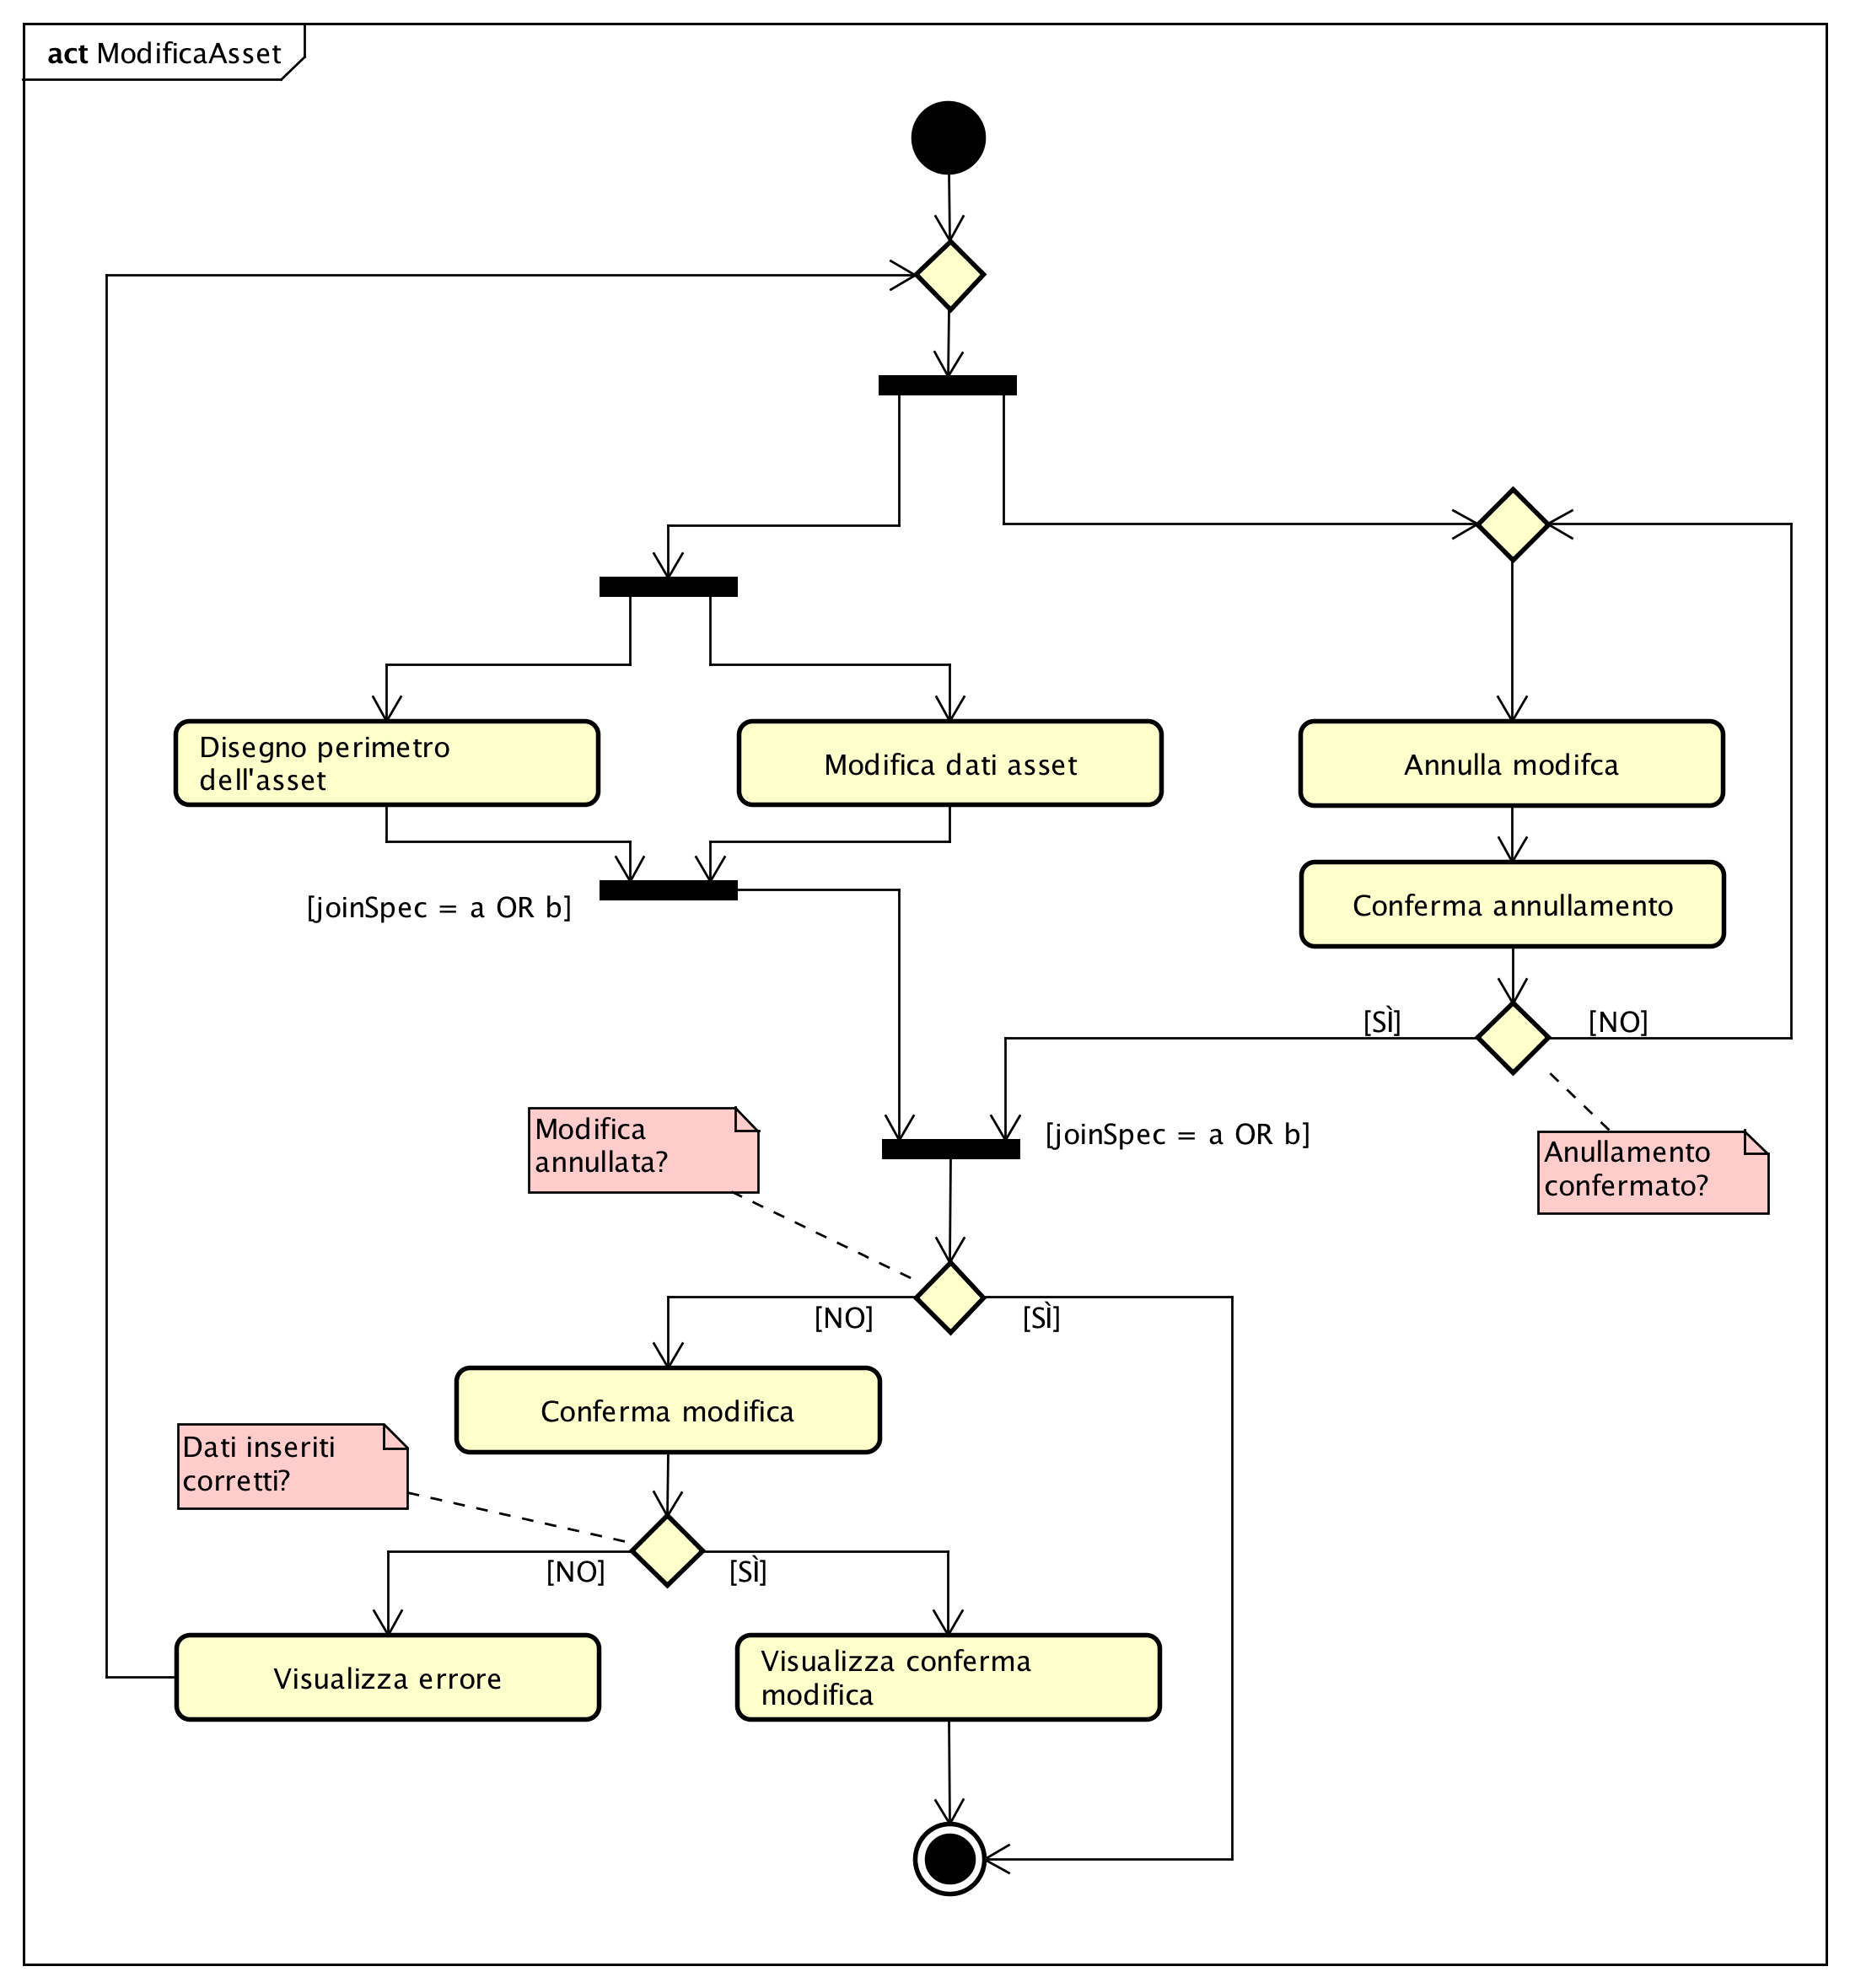
\includegraphics[width=\textwidth]{img/DiagrammiDiAttivita/ModificaAsset.png}
	\caption{Diagramma di attività per la modifica di un asset}
\end{figure}
\begin{figure}[H]
	\centering
	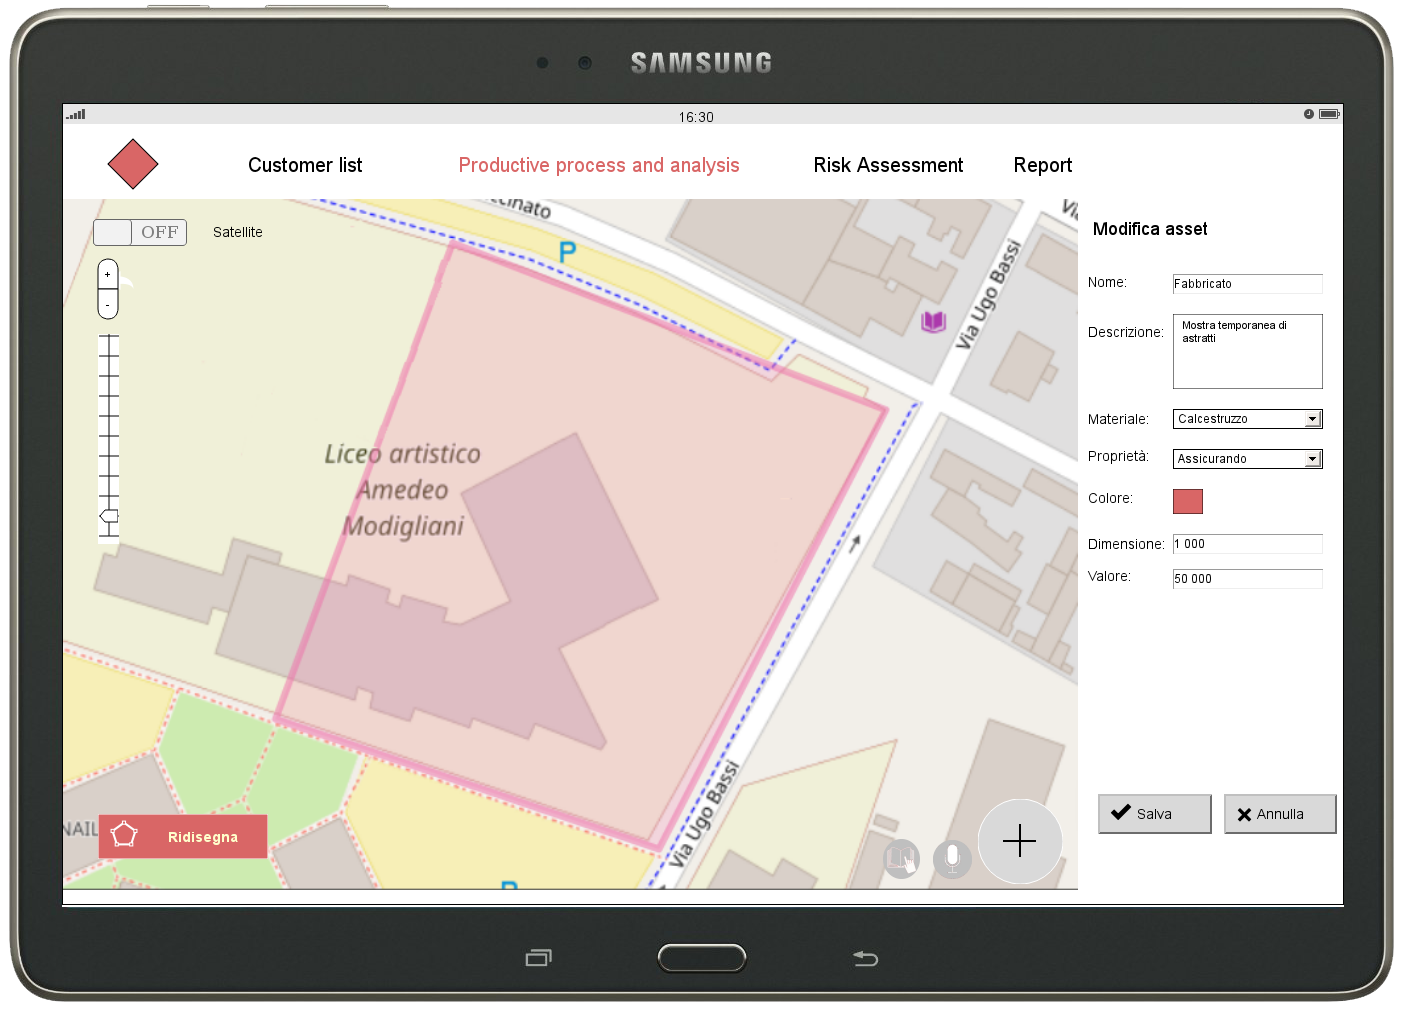
\includegraphics[width=\textwidth]{img/MockUp/m8.png}
	\caption{Mockup per la modifica di un asset}
\end{figure}

\newpage
\subsection{Modifica nodo}
Per quanto riguarda la modifica del nodo, sarà possibile riposizionare il nodo sulla mappa e/o modificarne i dati precedentemente compilati. Infine si dovrà confermare la modifica. In caso di dati non corretti, la modifica potrebbe non andare a buon fine: verrà visualizzato un messaggio di errore e l'utente sarà tenuto a correggere eventuali errori o incompletezze.
In ogni momento l'utente può annullare la modifica. Il sistema richiede una conferma per portare a termine tale operazione.
\begin{figure}[H]
	\centering
	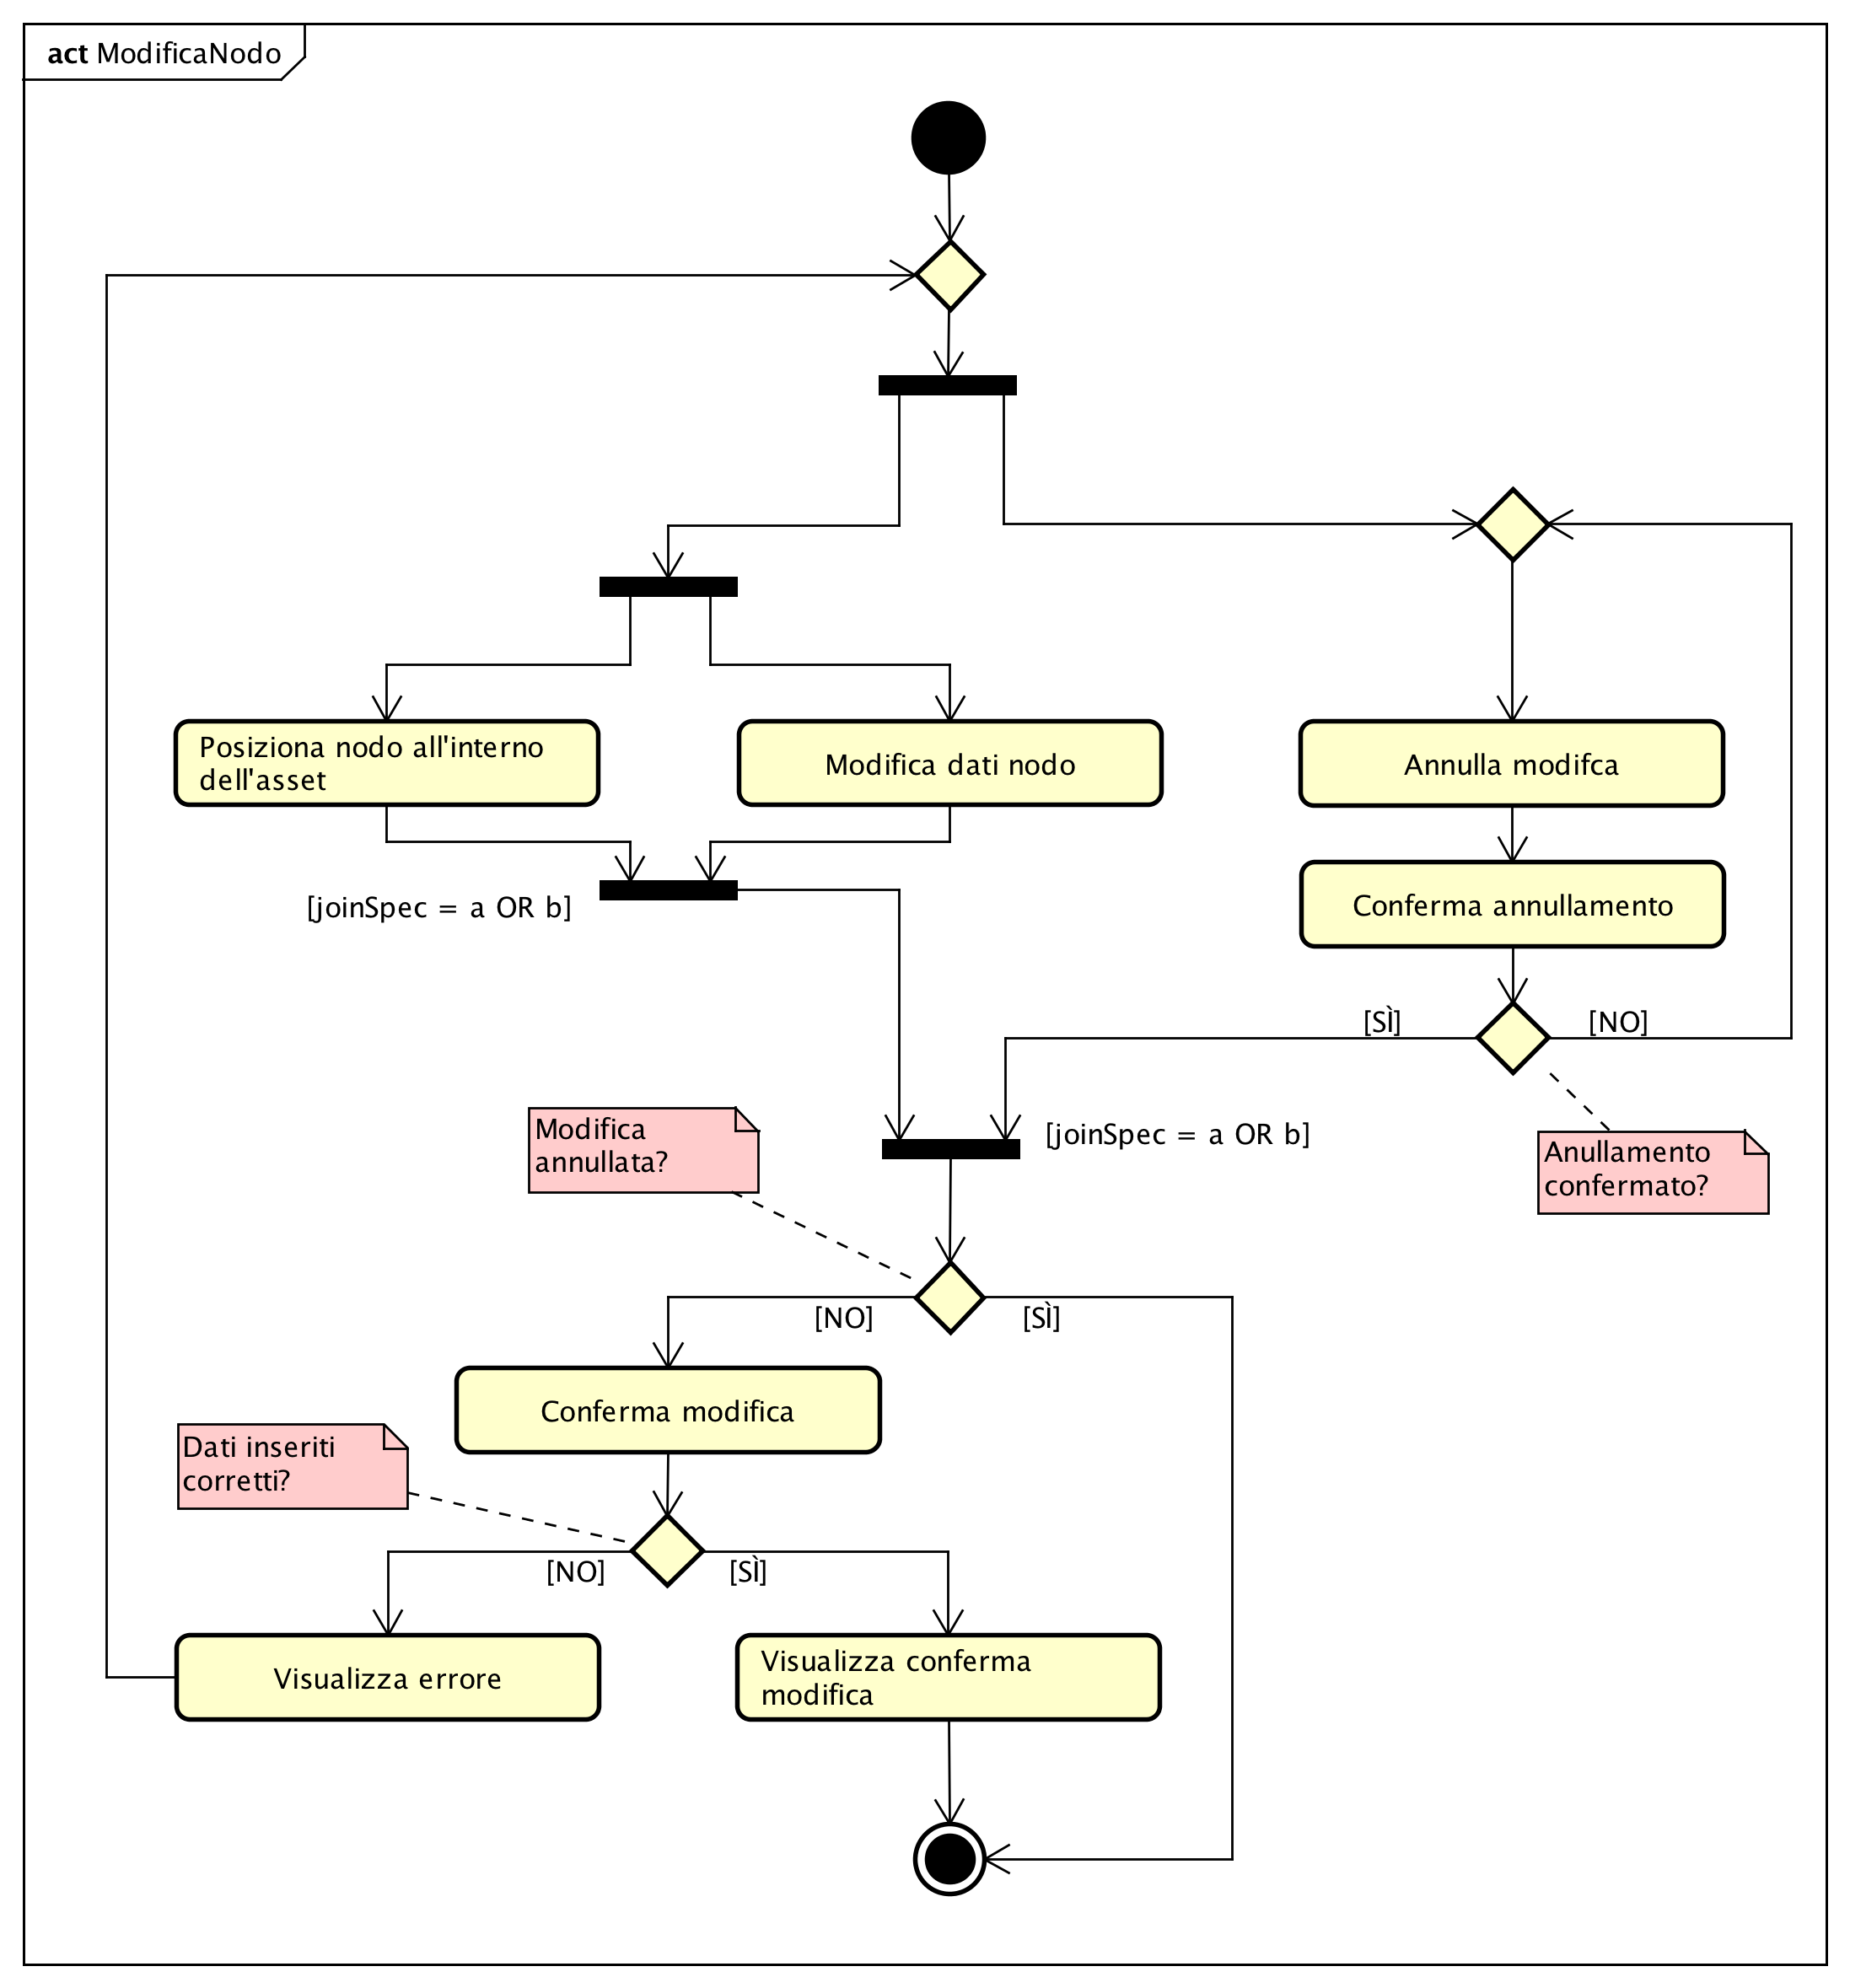
\includegraphics[width=\textwidth]{img/DiagrammiDiAttivita/ModificaNodo.png}
	\caption{Diagramma di attività per la modifica di un nodo}
\end{figure}
\begin{figure}[H]
	\centering
	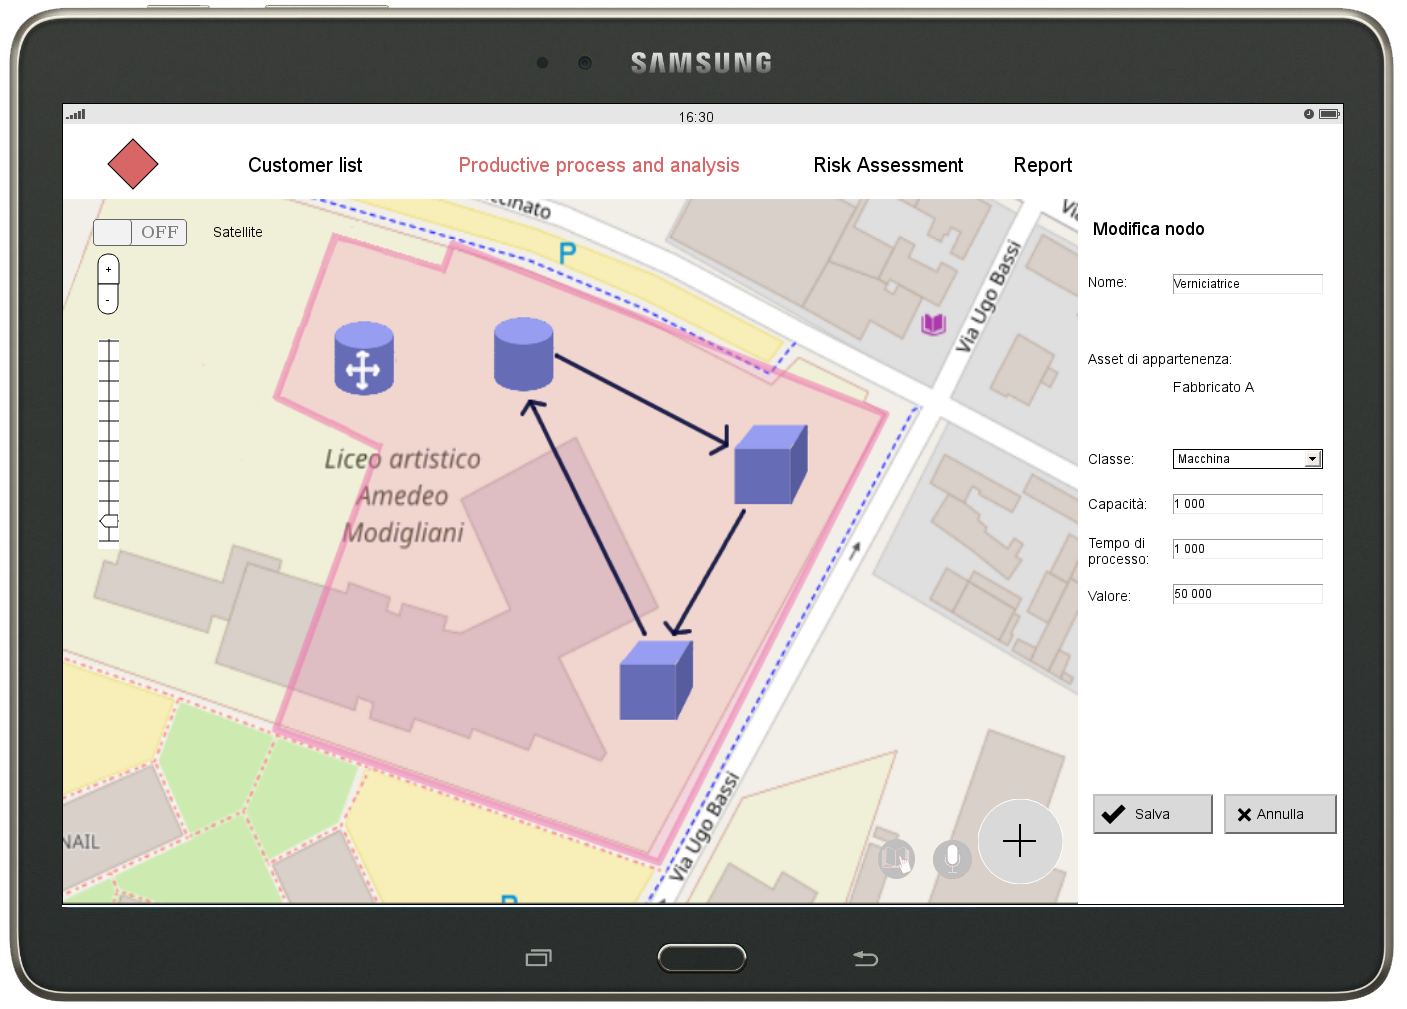
\includegraphics[width=\textwidth]{img/MockUp/m14.png}
	\caption{Mockup per la modifica di un nodo}
\end{figure}

\newpage
\subsection{Modifica arco}
Per quanto riguarda la modifica dell'arco, sarà possibile ridisegnare l'arco sulla mappa e/o modificarne i dati precedentemente compilati. Infine si dovrà confermare la modifica. In caso di dati non corretti, la modifica potrebbe non andare a buon fine: verrà visualizzato un messaggio di errore e l'utente sarà tenuto a correggere eventuali errori o incompletezze.
In ogni momento l'utente può annullare la modifica. Il sistema richiede una conferma per portare a termine tale operazione.
\begin{figure}[H]
	\centering
	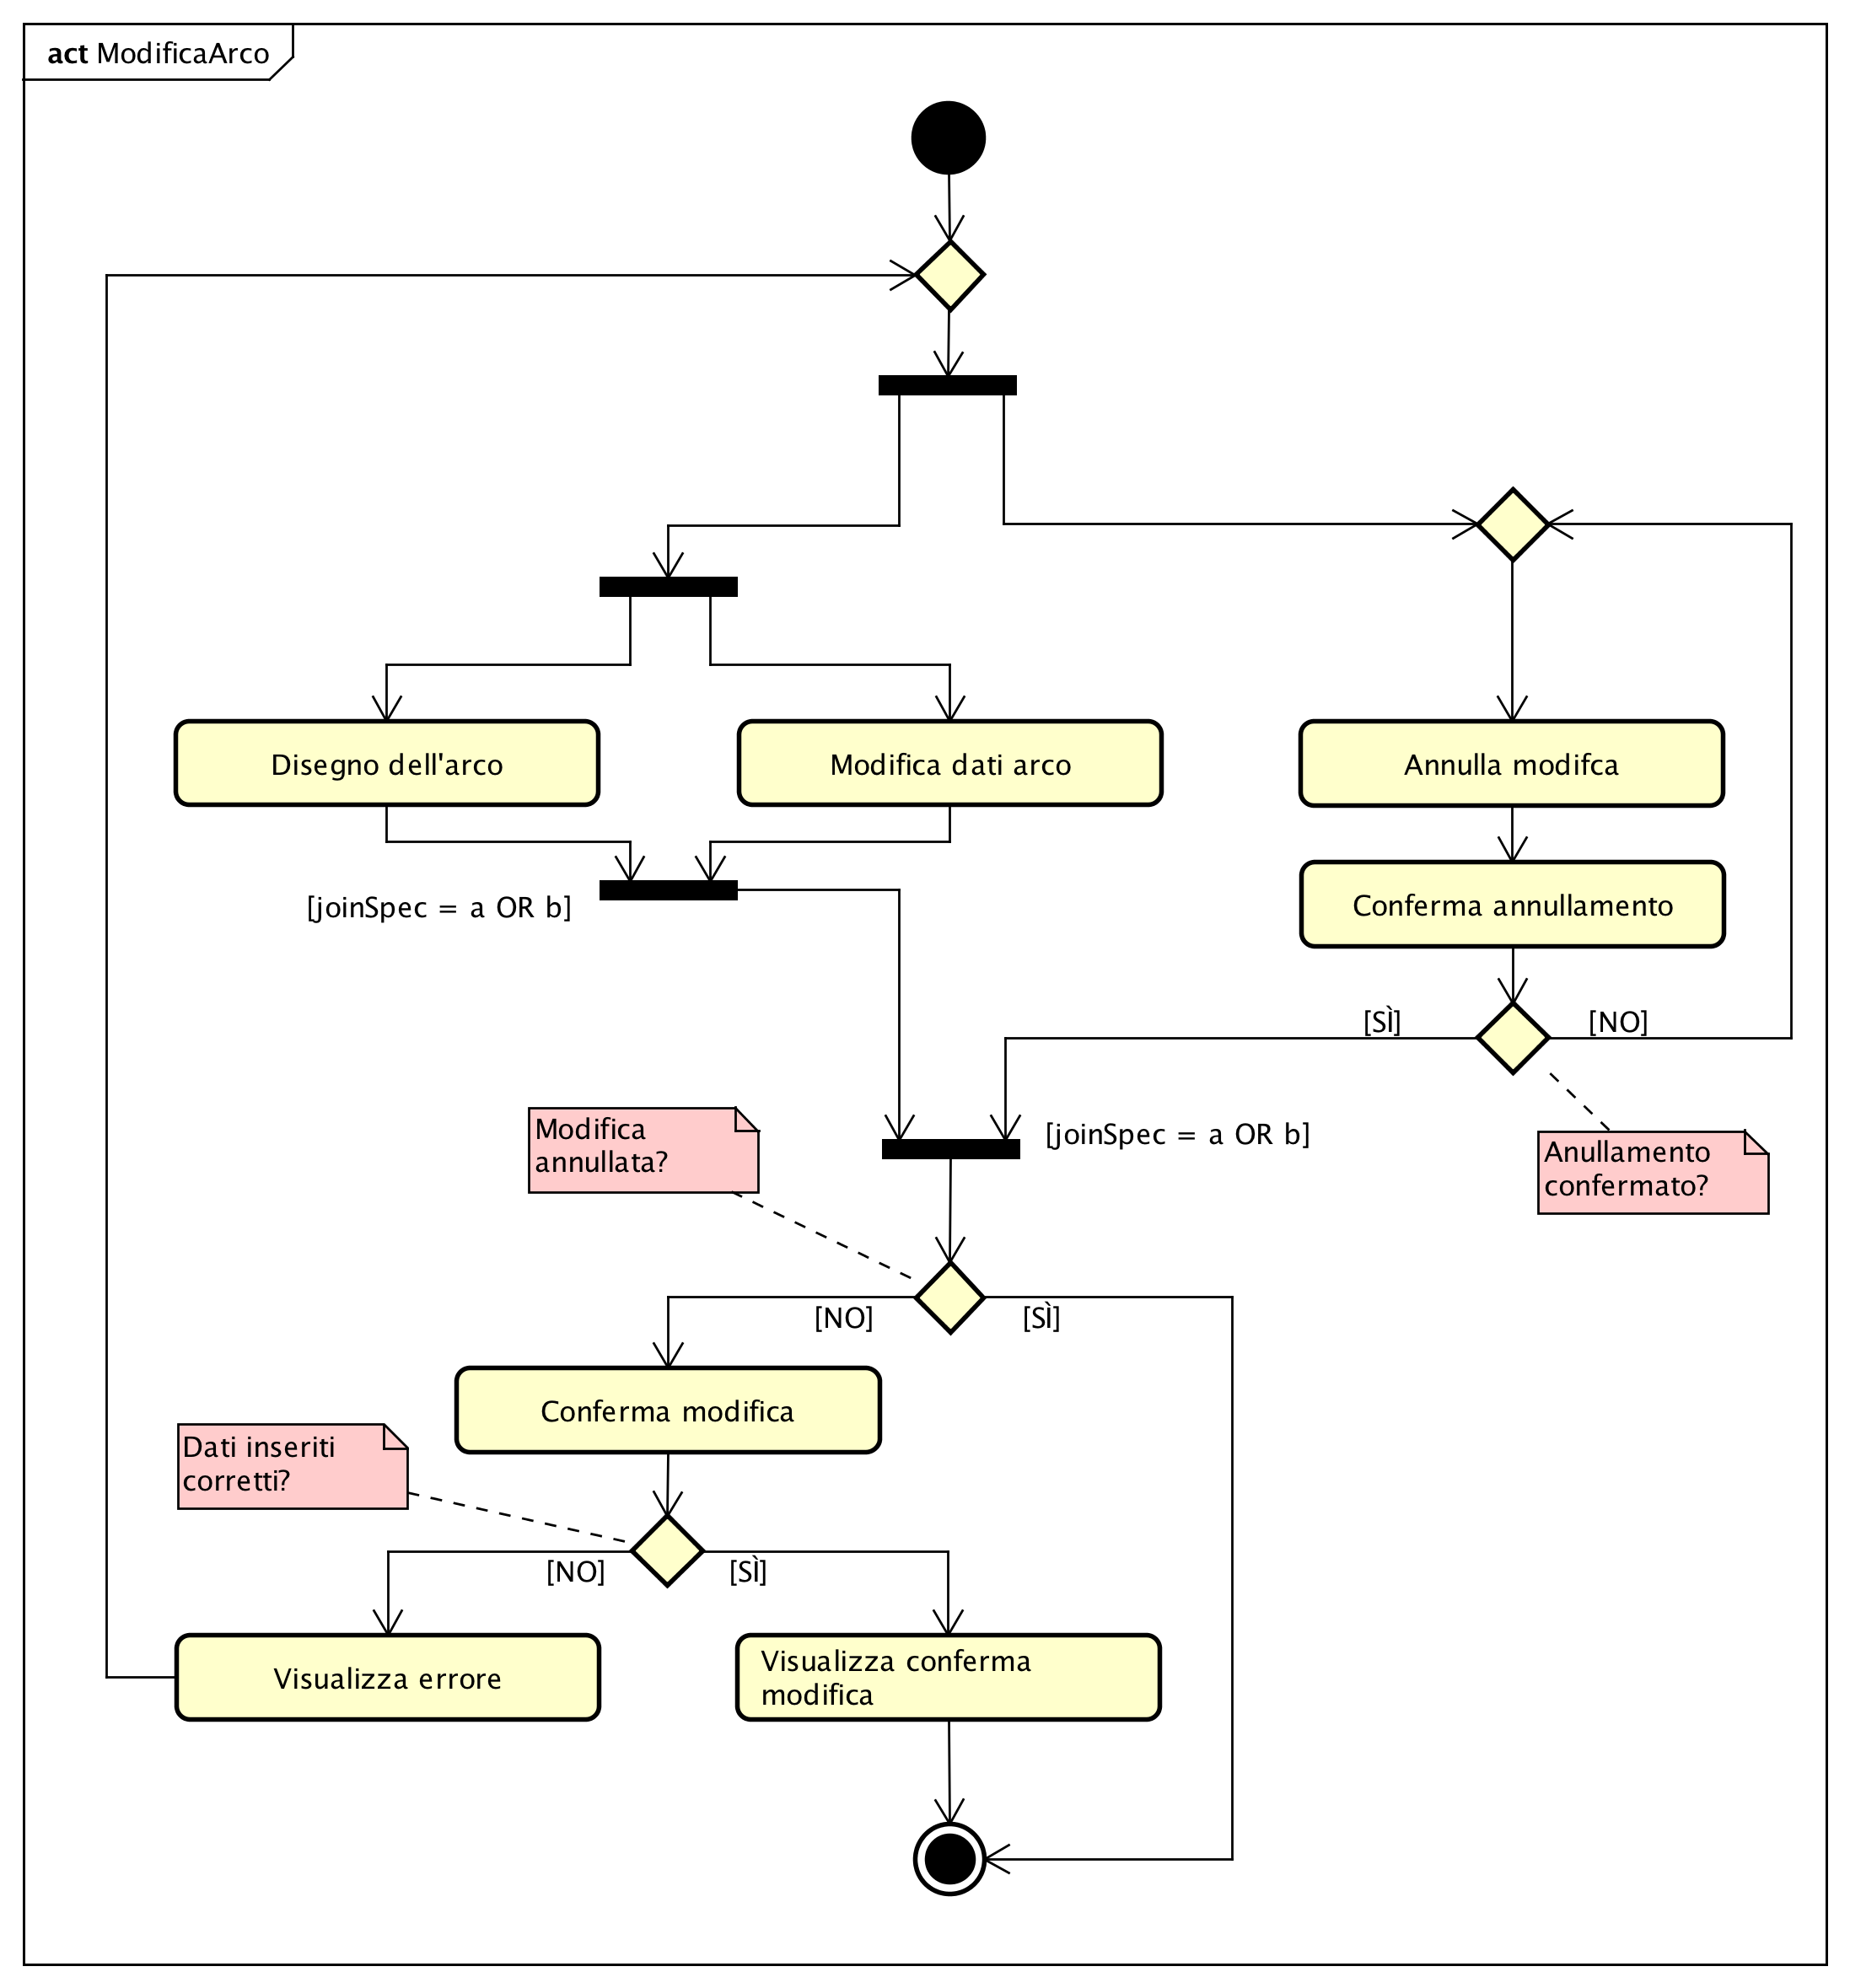
\includegraphics[width=\textwidth]{img/DiagrammiDiAttivita/ModificaArco.png}
	\caption{Diagramma di attività per la modifica di un arco}
\end{figure}

\newpage
\subsection{Modifica scenario}
Per quanto riguarda la modifica dello scenario, sarà possibile ridisegnarne il perimetro dell'asset sulla mappa e/o modificarne i dati precedentemente compilati. Infine si dovrà confermare la modifica. In caso di dati non corretti, la modifica potrebbe non andare a buon fine: verrà visualizzato un messaggio di errore e l'utente sarà tenuto a correggere eventuali errori o incompletezze.
In ogni momento l'utente può annullare la modifica. Il sistema richiede una conferma per portare a termine tale operazione.
\begin{figure}[H]
	\centering
	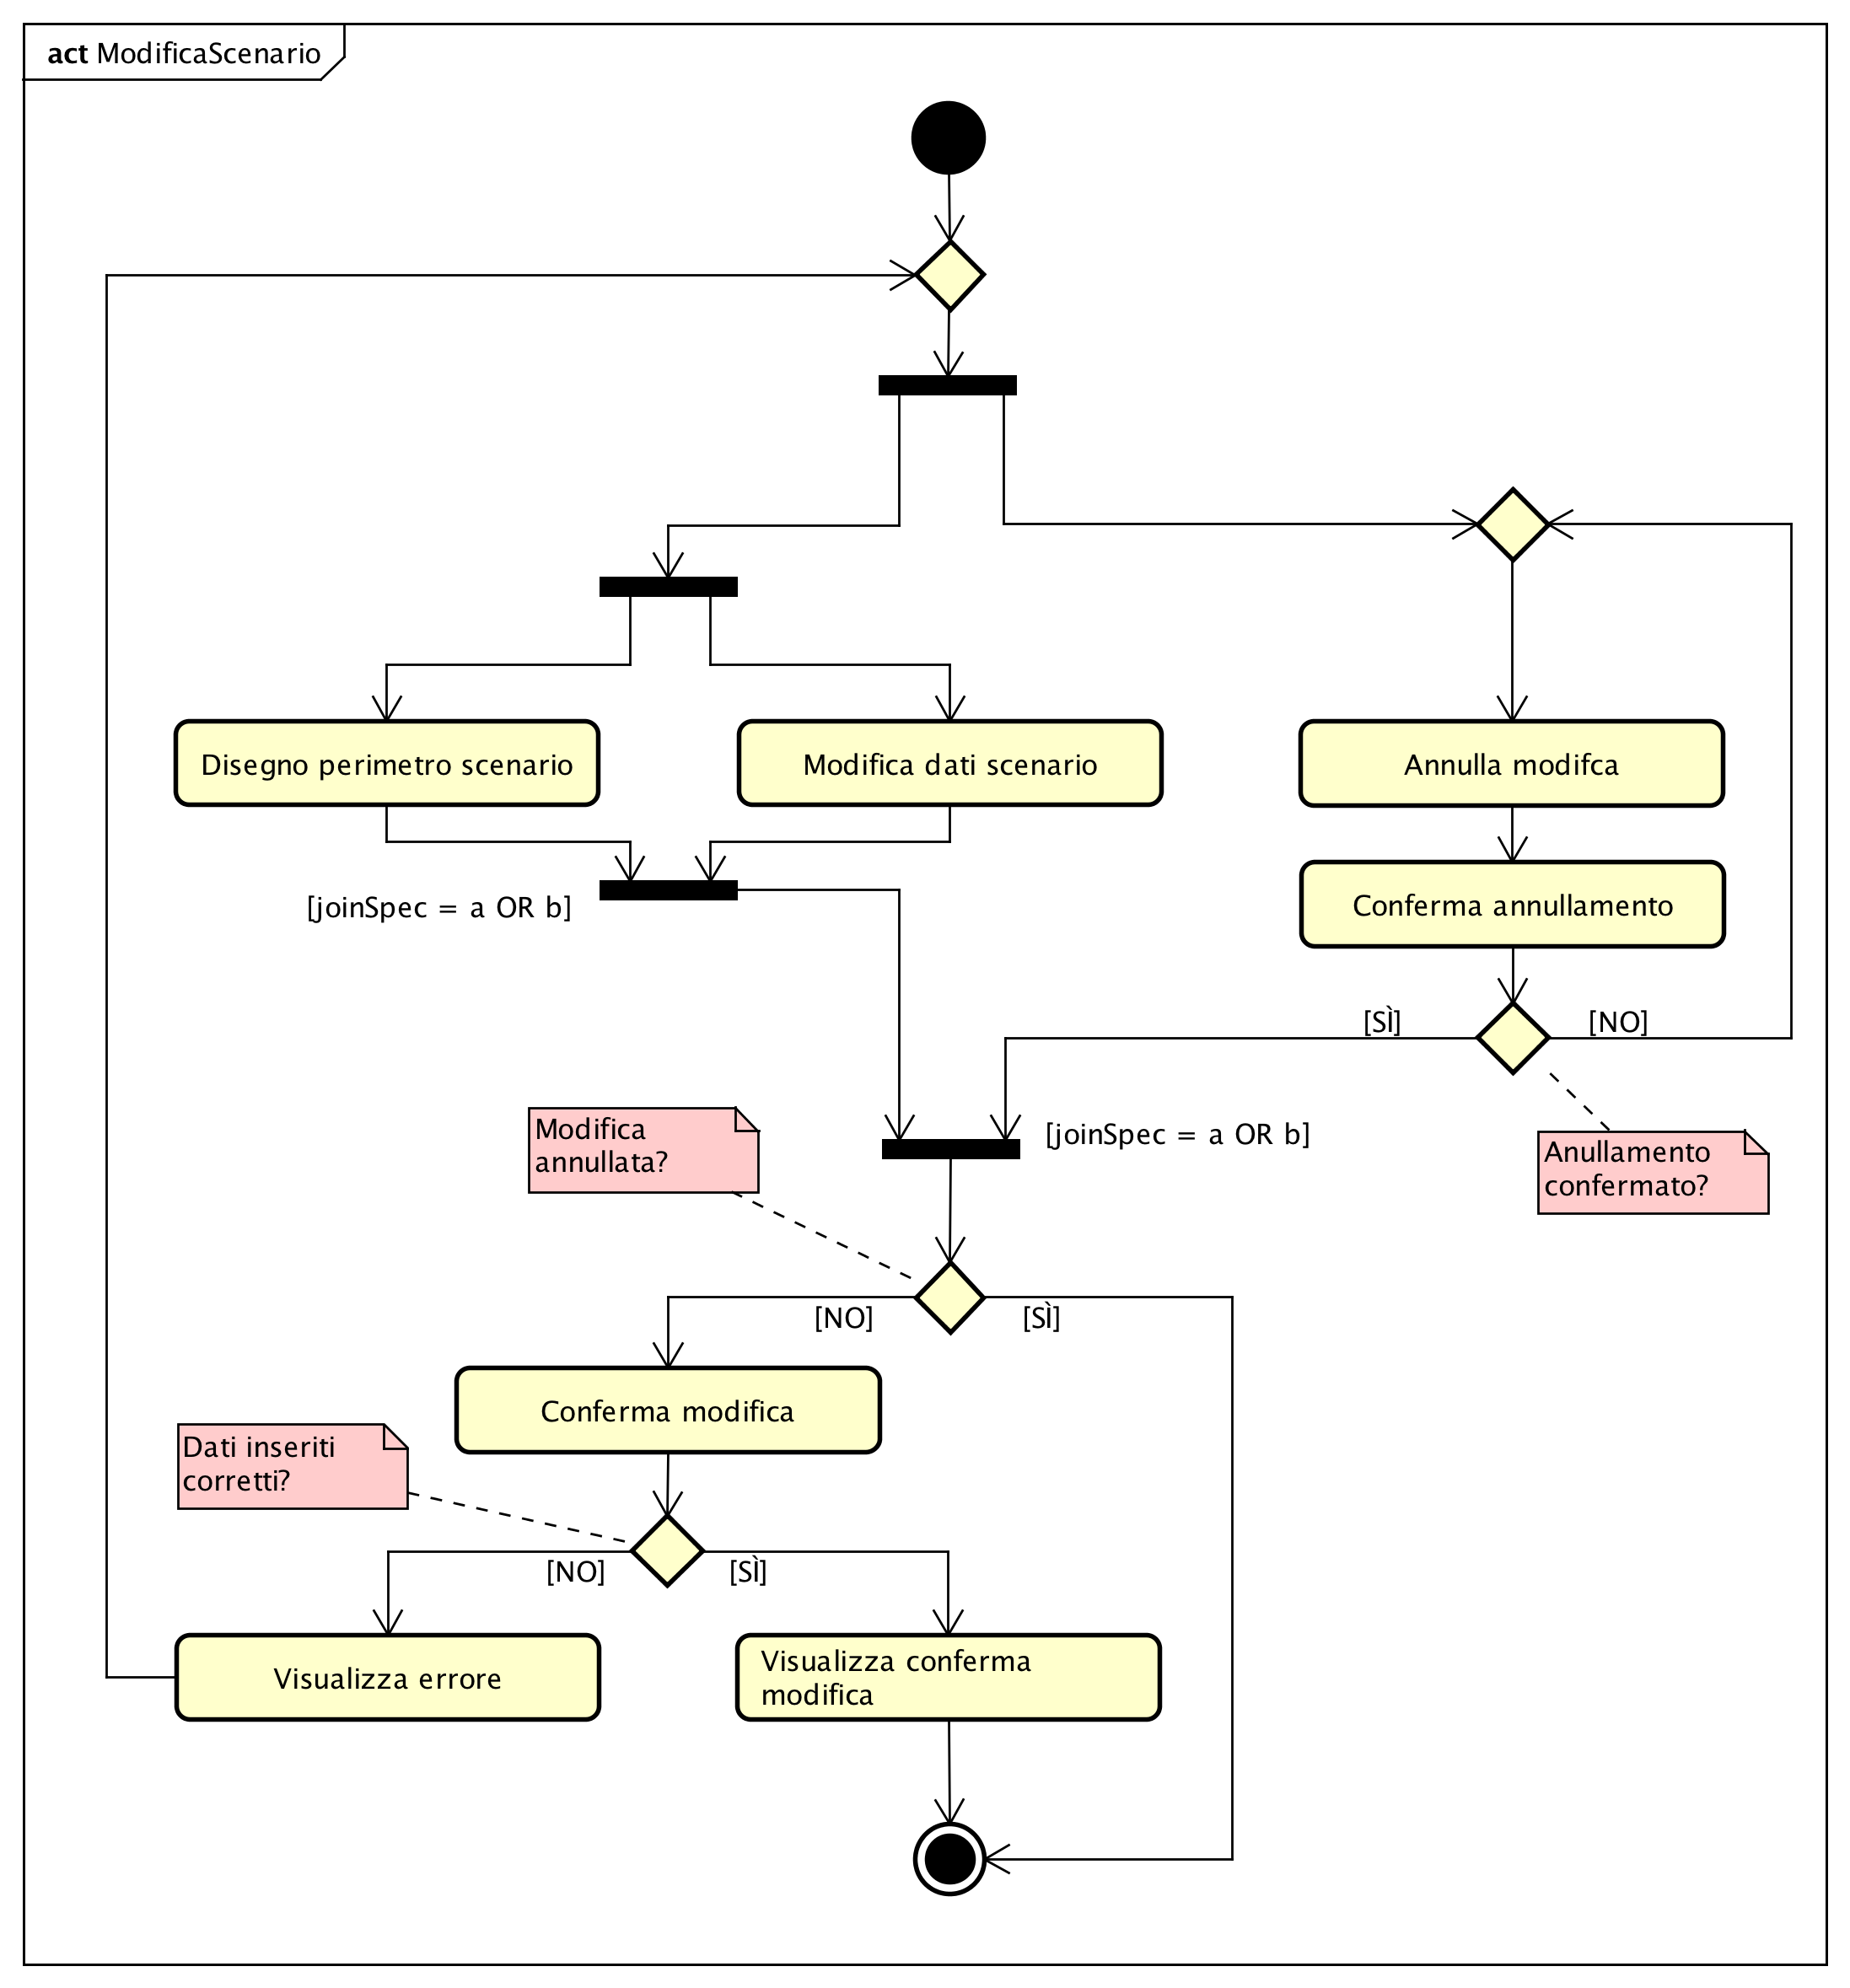
\includegraphics[width=\textwidth]{img/DiagrammiDiAttivita/ModificaScenario.png}
	\caption{Diagramma di attività per la modifica di uno scenario}
\end{figure}
\begin{figure}[H]
	\centering
	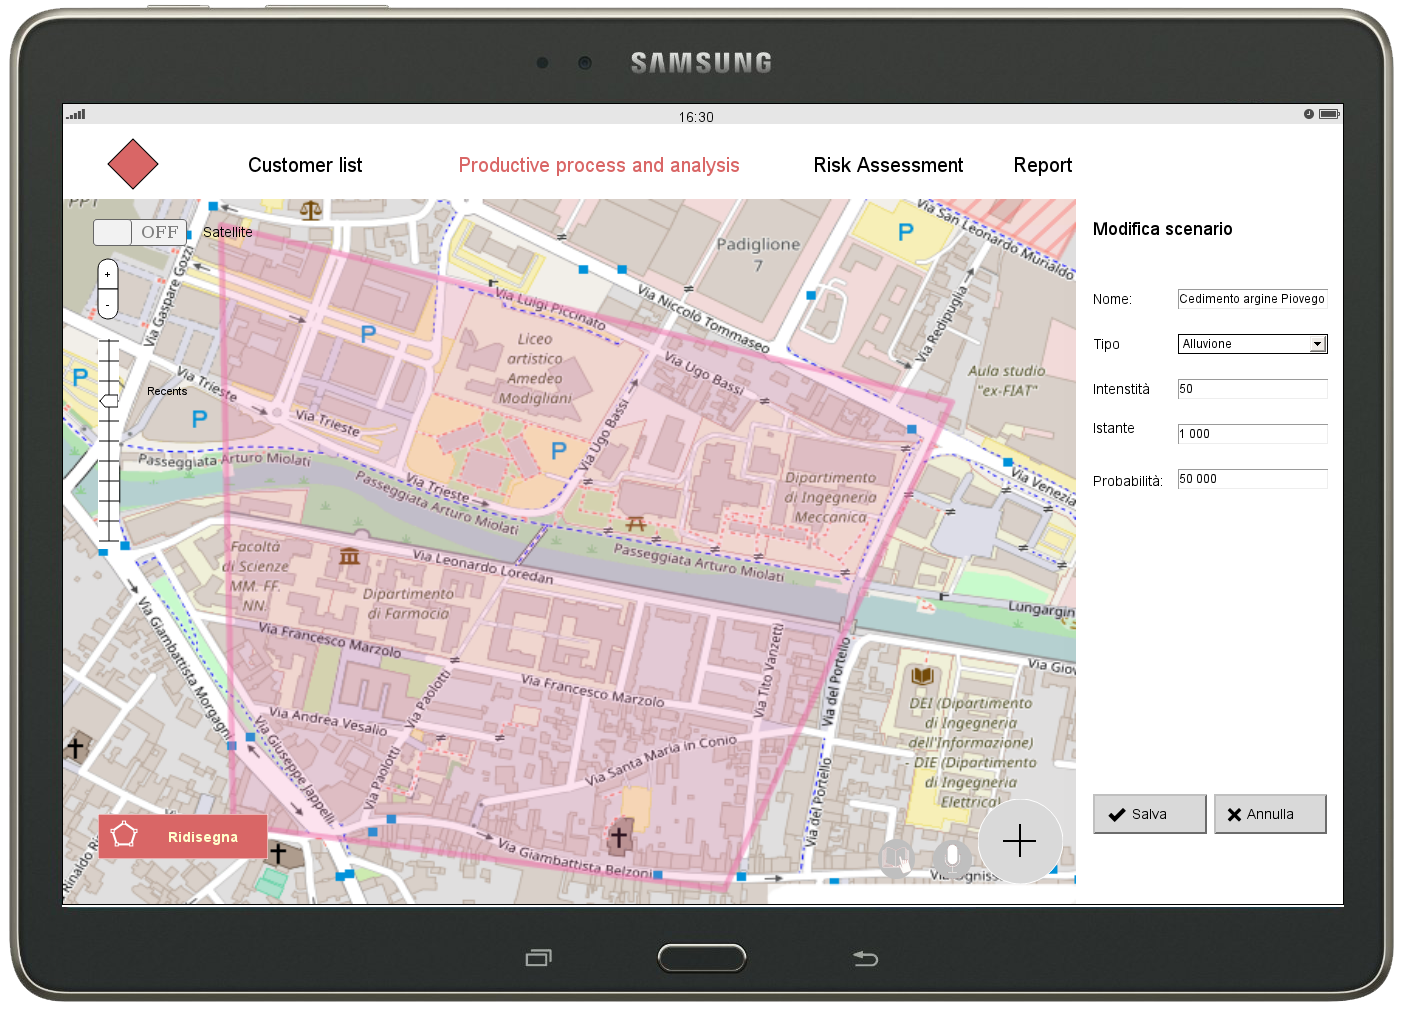
\includegraphics[width=\textwidth]{img/MockUp/m21.png}
	\caption{Mockup per la modifica di uno scenario}
\end{figure}

\newpage
\subsection{Eliminazione asset}
Una volta scelto di eliminare l'asset, l'utente è invitato a confermare l'eliminazione o ad annullarla.
\begin{figure}[H]
	\centering
	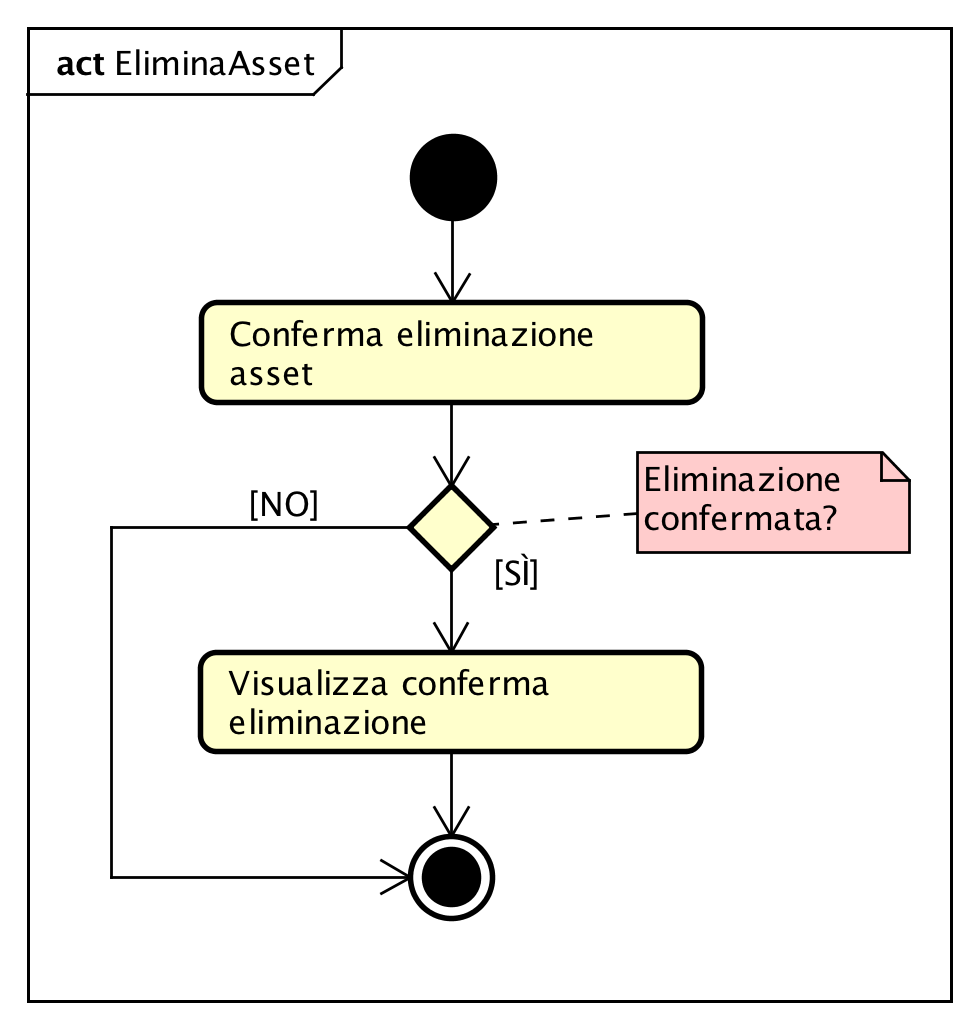
\includegraphics[scale=0.7]{img/DiagrammiDiAttivita/EliminazioneAsset.png}
	\caption{Diagramma di attività per l'eliminazione di un asset}
\end{figure}

\newpage
\subsection{Eliminazione nodo}
Una volta scelto di eliminare il nodo, l'utente è invitato a confermare l'eliminazione o ad annullarla.
\begin{figure}[H]
	\centering
	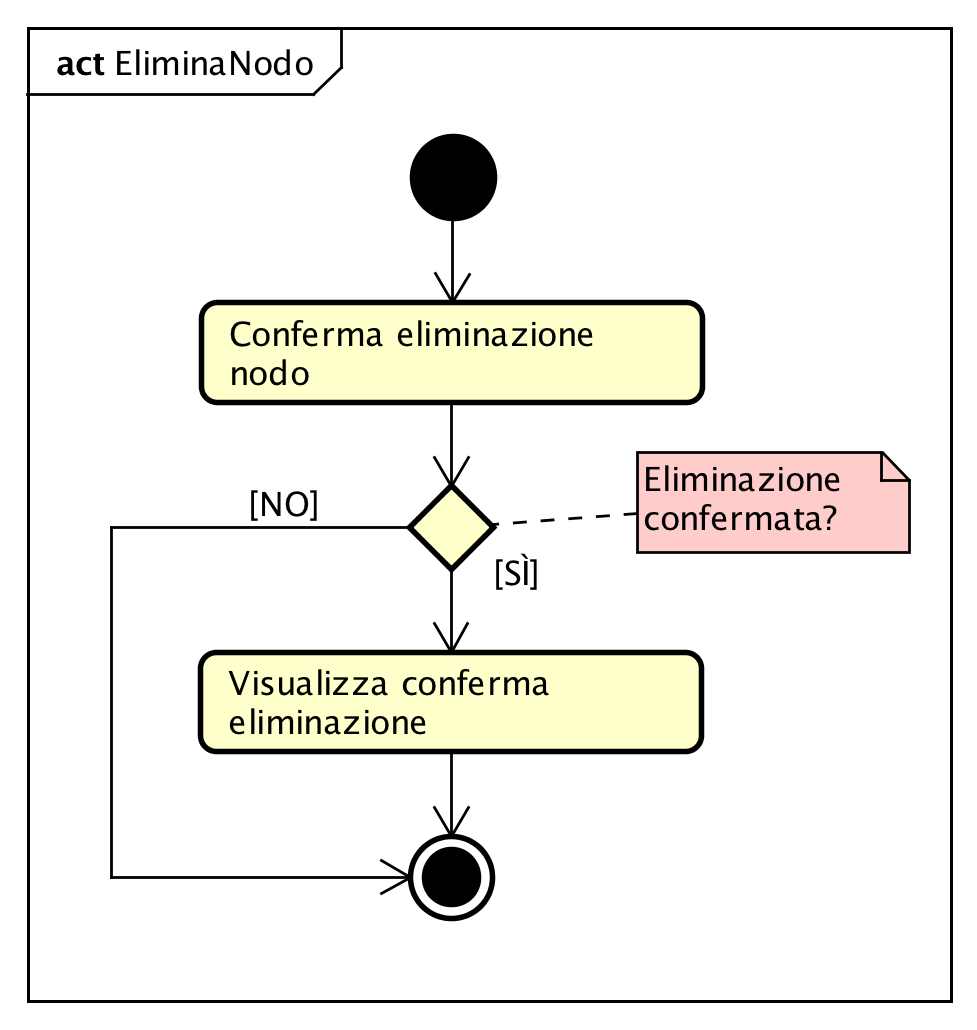
\includegraphics[scale=0.7]{img/DiagrammiDiAttivita/EliminazioneNodo.png}
	\caption{Diagramma di attività per l'eliminazione di un nodo}
\end{figure}
\begin{figure}[H]
	\centering
	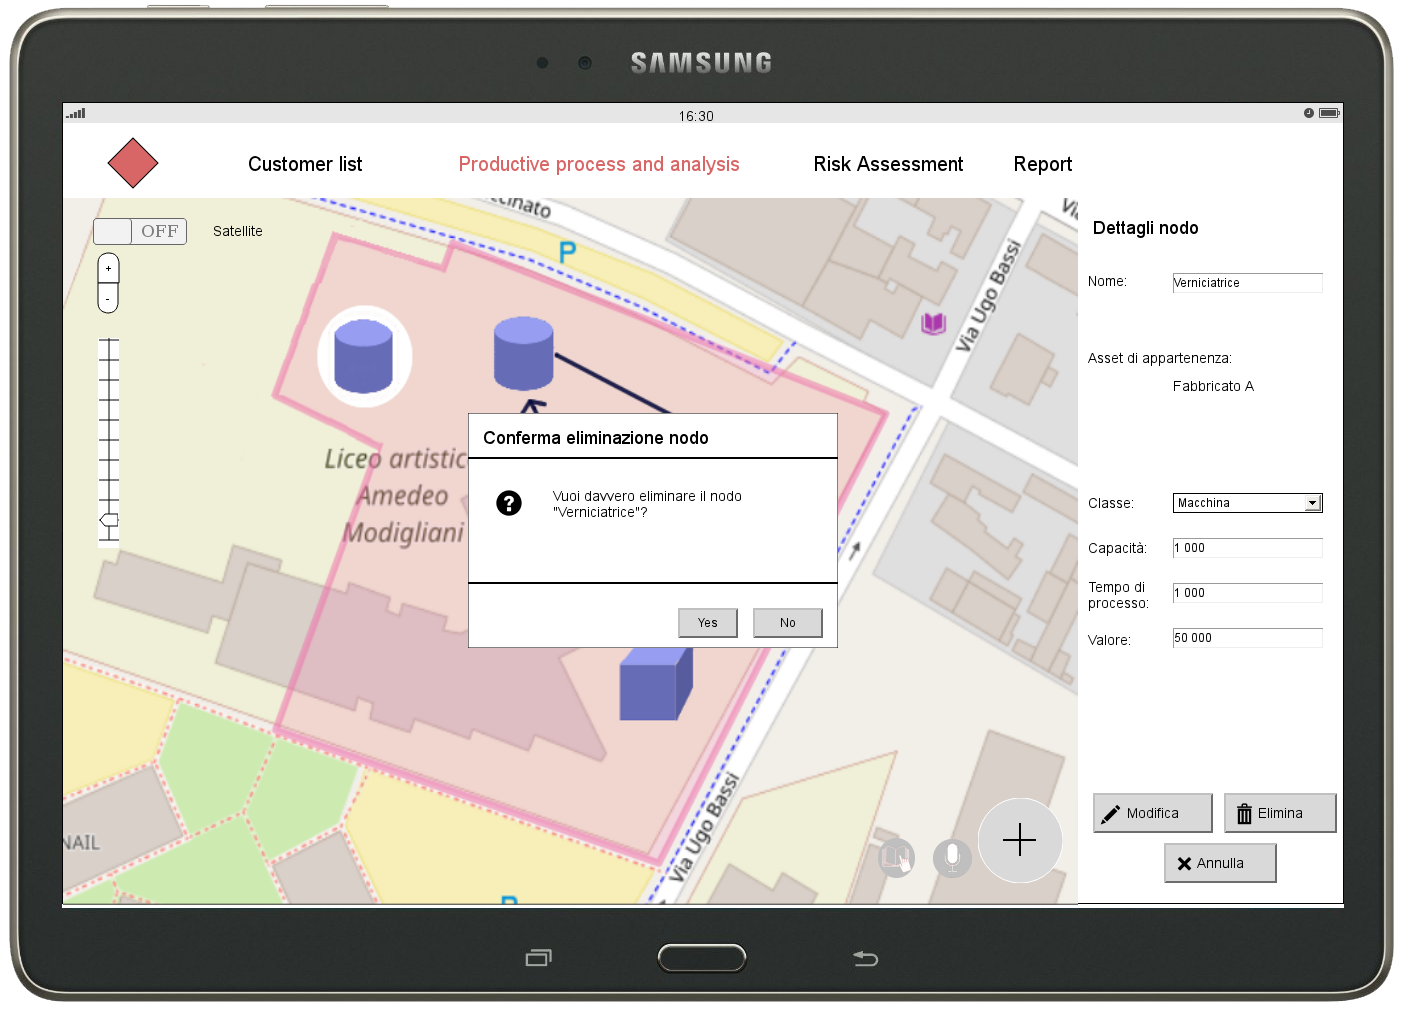
\includegraphics[width=\textwidth]{img/MockUp/m16.png}
	\caption{Mockup per l'eliminazione di un nodo}
\end{figure}


\newpage
\subsection{Eliminazione arco}
Una volta scelto di eliminare l'arco, l'utente è invitato a confermare l'eliminazione o ad annullarla.
\begin{figure}[H]
	\centering
	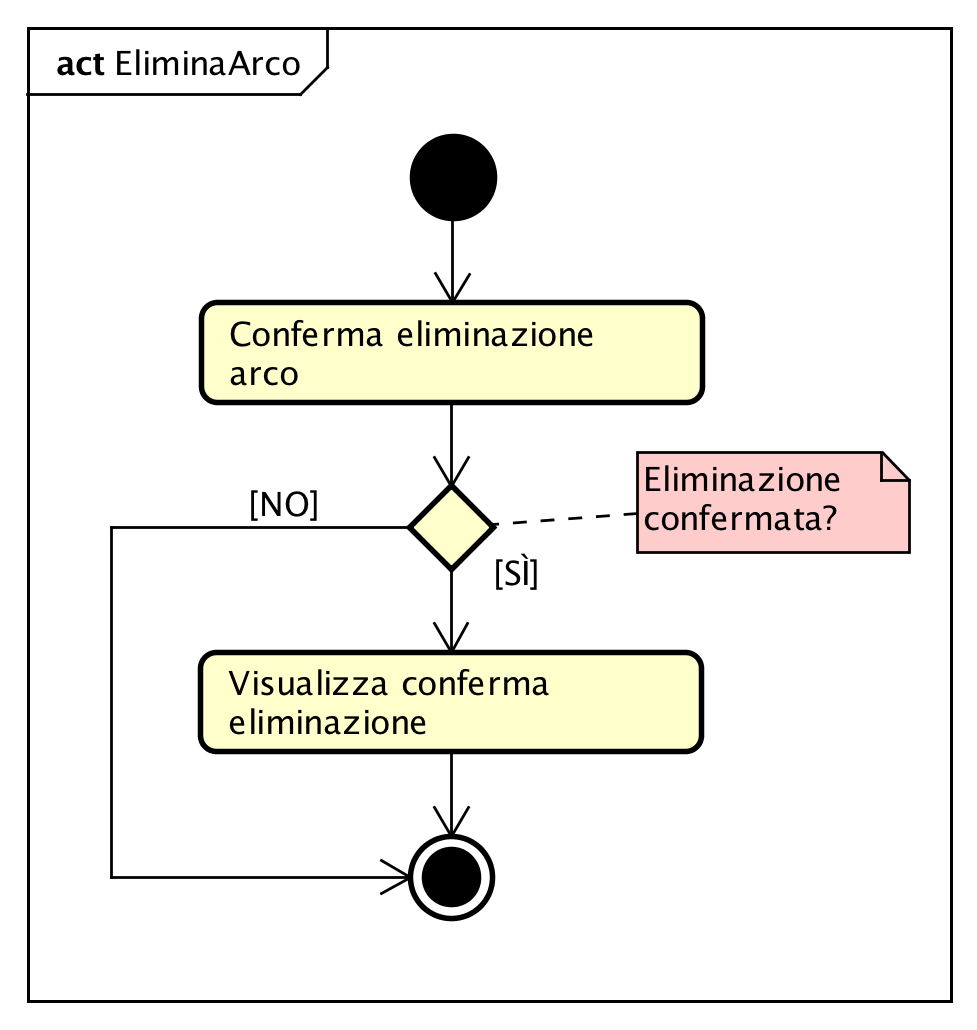
\includegraphics[scale=0.7]{img/DiagrammiDiAttivita/EliminazioneArco.png}
	\caption{Diagramma di attività per l'eliminazione di un arco}
\end{figure}

\newpage
\subsection{Eliminazione scenario}
Una volta scelto di eliminare lo scenario, l'utente è invitato a confermare l'eliminazione o ad annullarla.
\begin{figure}[H]
	\centering
	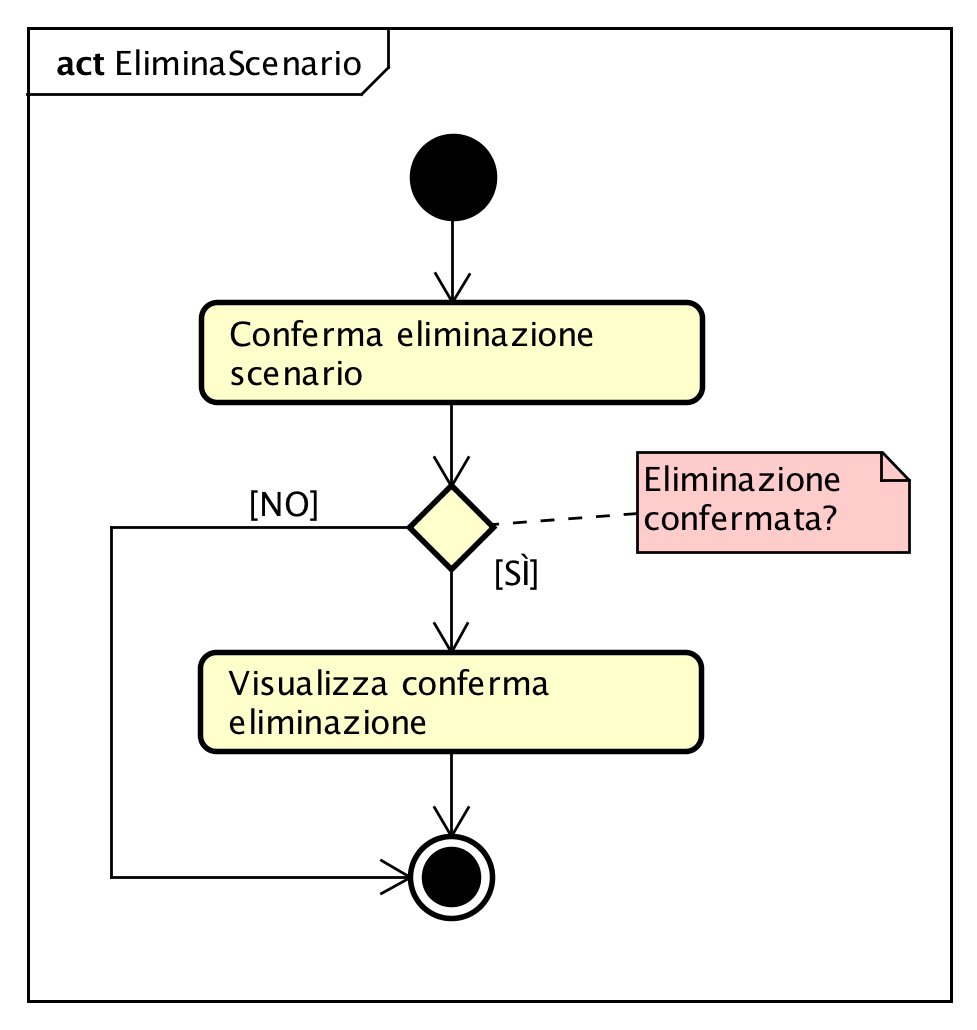
\includegraphics[scale=0.7]{img/DiagrammiDiAttivita/EliminazioneScenario.png}
	\caption{Diagramma di attività per l'eliminazione di uno scenario}
\end{figure}

\newpage
\subsection{Errore di connessione}
In caso di errori di connessione compare un messaggio di errore. In questo caso l'utente può chiudere la visualizzazione del messaggio di errore o ricaricare la pagina.
\begin{figure}[H]
	\centering
	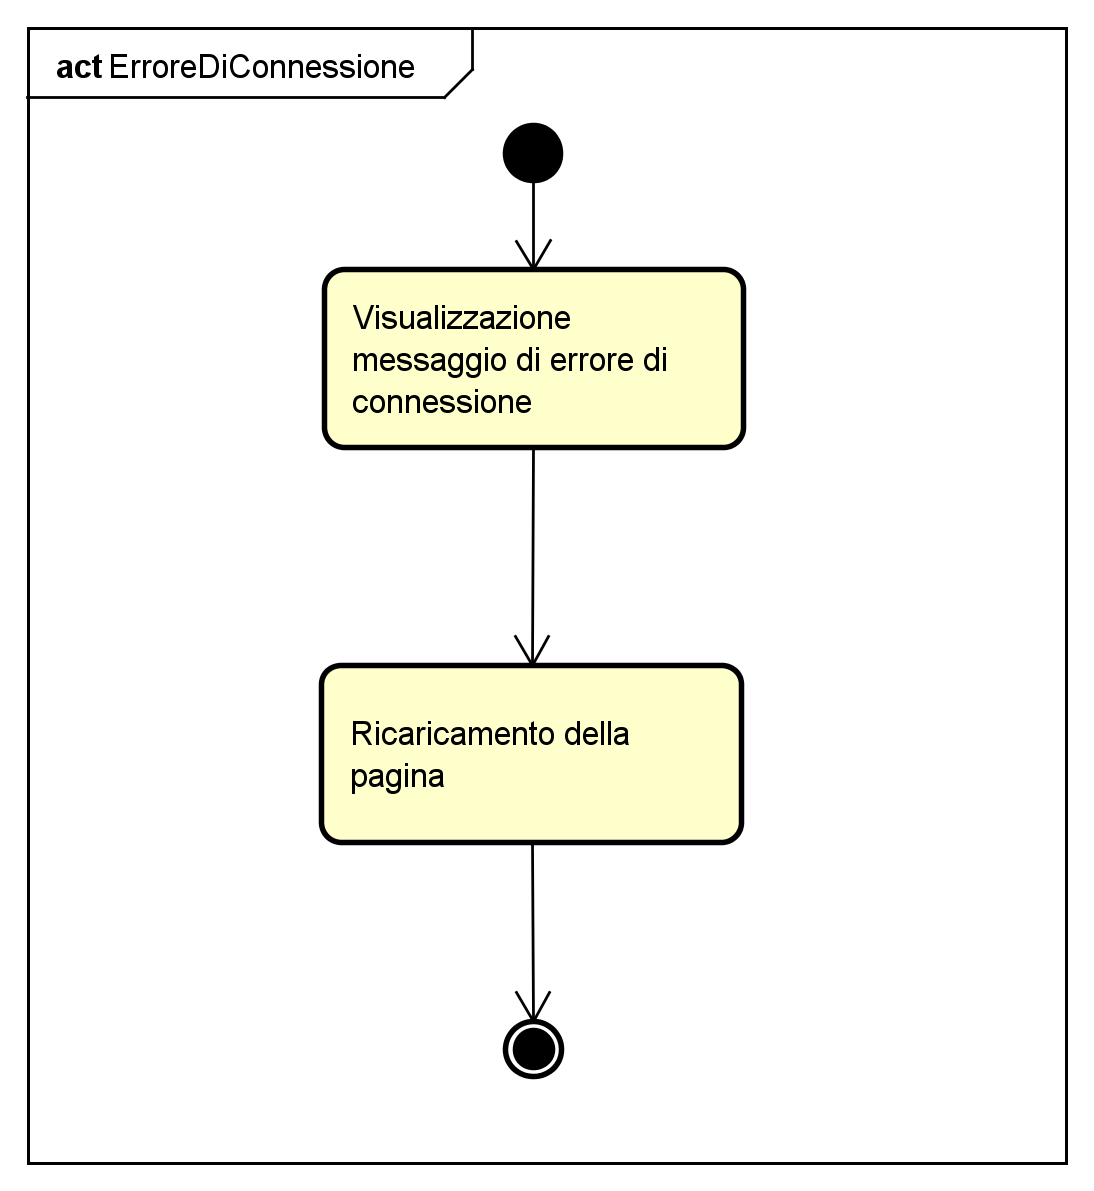
\includegraphics[scale=0.7]{img/DiagrammiDiAttivita/ErroreDiConnessione.png}
	\caption{Diagramma di attività per l'eliminazione di un nodo}
\end{figure}
\begin{figure}[H]
	\centering
	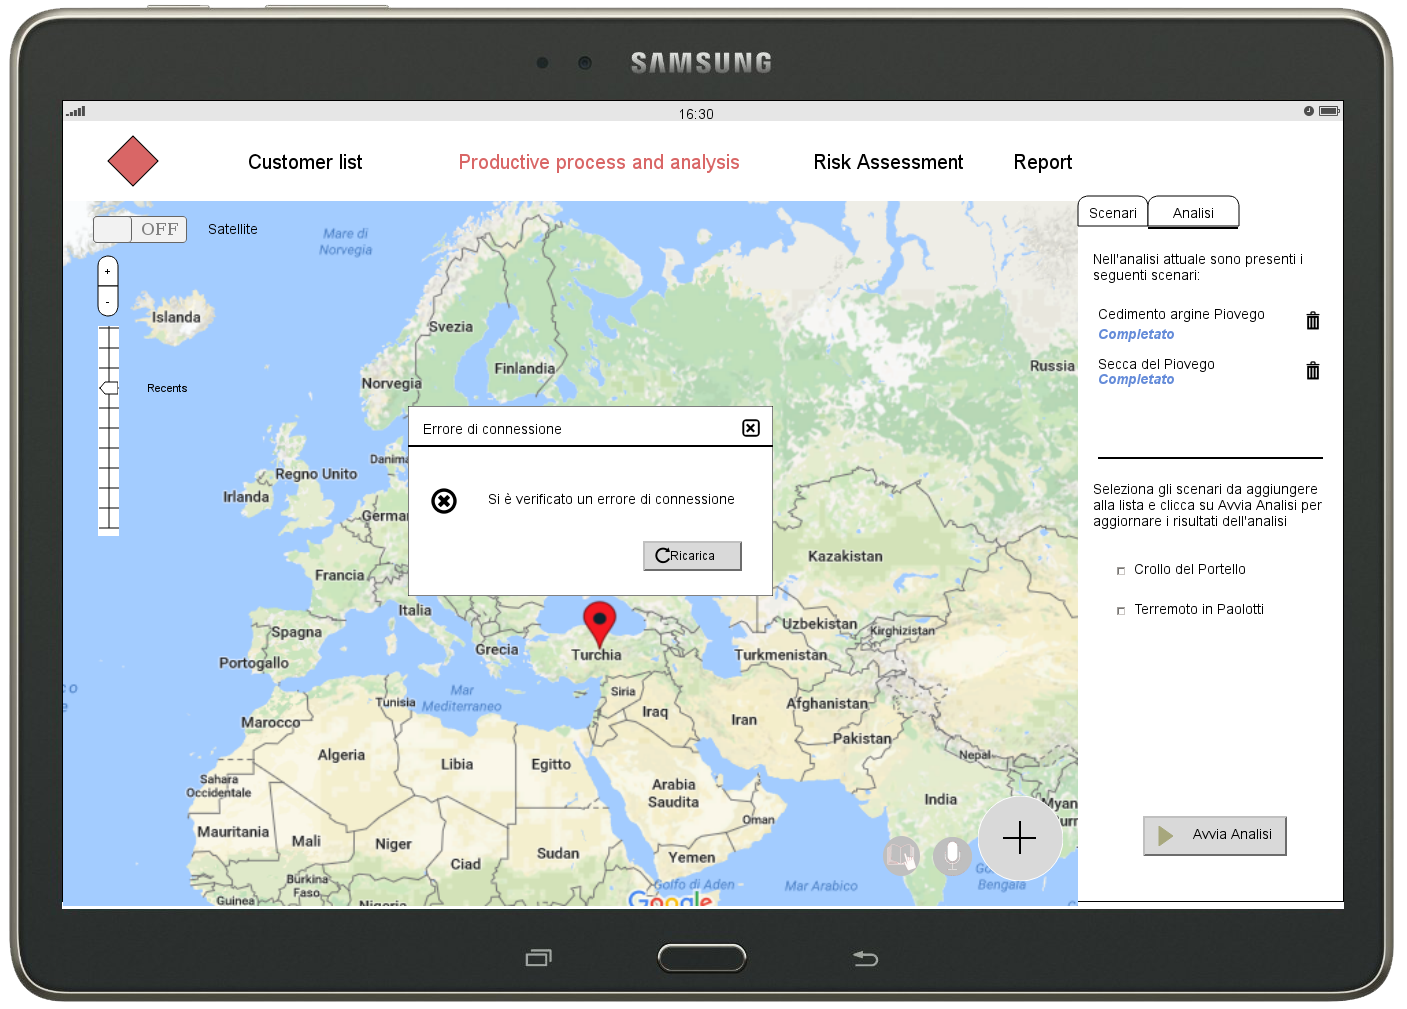
\includegraphics[width=\textwidth]{img/MockUp/m9.png}
	\caption{Mockup per gli errori di connessione}
\end{figure}